\documentclass[12pt,draft]{VTthesis}
\usepackage{elf}
\usepackage{wrapfig}
\usepackage{subcaption}

\title{
  Finite Elements for the Quasi-Geostrophic Equations of the Ocean
}

\keywords{Quasi-geostrophic equations, finite element method, Argyris element,
wind-driven ocean currents.}

\author{Erich L Foster}
\program{Mathematics}
\degree{Doctor of Philosophy}
\type{Proposal}
\submitdate{17 April 2013}
\principaladvisor{Traian Iliescu}
\firstreader{Slimane Adjerid}
\secondreader{John A. Burns}
\thirdreader{Anne Staples}

%\dedication{This is where you put your dedications.}
%\acknowledge{This is where you put your acknowledgments.}

\abstract{
  The quasi-geostrophic equations (QGE) are usually discretized in space by the
  finite difference method, however, the finite element (FE) method offers
  several advantages of the finite difference method such the easy treatment of
  complex boundaries and a natural treatment of boundary conditions
  \cite{Myers}. Despite these advantages, there are relatively few papers that
  consider the FE method applied to the QGE.

  To our knowledge, \emph{all} FE discretizations of the QGE have been developed
  for the streamfunction-vorticity formulation, none using the streamfunction
  formulation. The reason is simple: The streamfunction-vorticity formulation
  yields a second order \emph{partial differential equation (PDE)}, whereas the
  streamfunction formulation yields a fourth order PDE. Thus, although the
  streamfunction-vorticity formulation has two variables ($q$ and $\psi$) and
  the streamfunction formulation has just one ($\psi$), the former is the
  preferred formulation used in practical computations, since its conforming FE
  discretization requires low-order ($C^0$) elements, whereas the latter
  requires a high-order ($C^1$) FE discretization.

  We present a conforming FE discretization of the QGE based on the Argyris
  element and we present a two-level FE discretization of the Stationary QGE
  (SQGE) based on the same conforming FE discretization using the Argyris
  element. We also, \emph{for the first time}, develop optimal error estimates
  for the QGE. Numerical tests for the FE discretization and the two-level FE
  discretization of the QGE are presented and theoretical error estimates are
  verified. By benchmarking the numerical results against those in the published
  literature, we conclude that our FE discretization is accurate.  Furthermore,
  the numerical results have the same convergence rates as those predicted by
  the theoretical error estimates.
}

\begin{document}
  \frontmatter
  \maketitle
  \tableofcontents
  \listoftables
  \listoffigures

  \mainmatter

  \chapter{Introduction} \label{ch:Intro}
    \section{Motivation} \label{sec:Motivation}
    Ocean currents have influenced humanity since the beginning of time, both through the effects
ocean currents have on climate, but also through the effects they have on human travel. Vikings and
Polynesians both made use of ocean currents in their exploration \cite{Dijkstra08, Ingstad}. The
Vikings used the ocean currents to travel between Europe and the Americas \cite{Ingstad}. In fact,
the Vikings were able to sail all along the Greenland coast, because of a lack of ice bergs caused
by a more northerly reaching Gulf Stream, which receded a century later \cite{Morner95}.

The first documentation of ocean currents were made by Christopher Columbus (1492-1494), Vasco da
Gama (1497-1499), and Ferdinand Magellan (1519-1522). In fact, the Gulf Stream was first mapped by
Benjamin Franklin in 1769 (\autoref{fig:Franklin}) \cite{Dijkstra08, Vallis06}. The first
instrumental observations of ocean currents on a global scale were begun by the HMS
\emph{Challenger} in 1872 when she set sail for over three years around the world \cite{Siedler01}.

\begin{figure}[H] 
  \begin{center}
    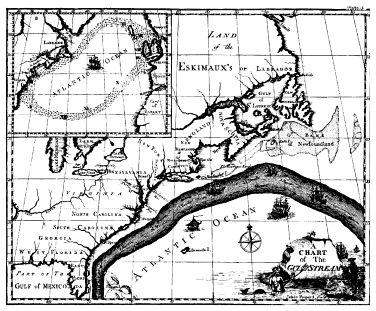
\includegraphics[scale=0.5]{Franklin-Folger.png}
    \caption{Map of the Gulf Stream by Franklin-Folger, 1769}
    \label{fig:Franklin}
  \end{center}
\end{figure}

In more recent times we read of plans for shipping through the Northwestern Passage, which until
recently had been closed by sea ice. Numerical climate models predicted that the passage would
eventually open, however the passage has opened much earlier than anticipated \cite{NatGeo}. Canada
claims it has full rights to the passage while the United States and Europe claim it is part of
international waters. On the other hand Russia has laid claims to the sea floor in the artic and
thereby raising tensions in the region. Clearly, climate change can influence geopolitics.  

The climate system is driven by energy from the sun. This solar energy is transfered from the low
latitudes to the high latitudes via radiative processes, and oceanic and atmosphic circulations. The
oceans make up approximately $71\%$ of the Earths surface, therefore the absorption of solar energy
is dominated by the oceans. Thus, climate variability is, to a large extent, an ocean-related
phenomenon \cite{Siedler01}. Because of this we see that ocean circulation changes are strongly
linked to changes in climate \cite{Morner95, Siedler01}. In fact, the cold periods in Western Europe
during the time periods 1440-1460, 1687-1703, and 1808-1821 can all be linked to a southward
deflection of the Gulf Stream and a southward penetration of Arctic cold water \cite{Morner95}.

%Two of the most important features of oceanic flows is the effects of rotation and stratification
%\cite{Majda}.

The large scale ocean flows are characterized by three major features: the wind forcing,
stratification, and the effects of rotation \cite{Majda, Vallis06}. Annual mean wind patterns,
where winds are westerward near the equator and eastward at the midlatitudes \cite{Dijkstra08},
drive the subtropical and subpolar gyres, which correspond to the strong, persistent, sub-tropical
and sub-polar western boundary currents: in the North Atlantic (the Gulf Stream and the Labrador
Current), in the South Atlantic (the Brazil and the Falkland Currents), in North Pacific (the
Kuroshio and the Oyashio Currents), in the South Pacific (East Australia Current) and in the Indian
Ocean (the Agulhas Current) \cite{Dijkstra08,Vallis06}. These major ocean currents are dipicted in
\autoref{fig:Currents}. One of the common features of these gyres is that they display strong
western boundary currents, weaker interior flows, and weak eastern boundary currents. Its these
wind-driven ocean circulations that play a significant role in climate dynamics
\cite{Dijkstra05,Ghil08}.

\begin{figure}[H] 
  \begin{center}
    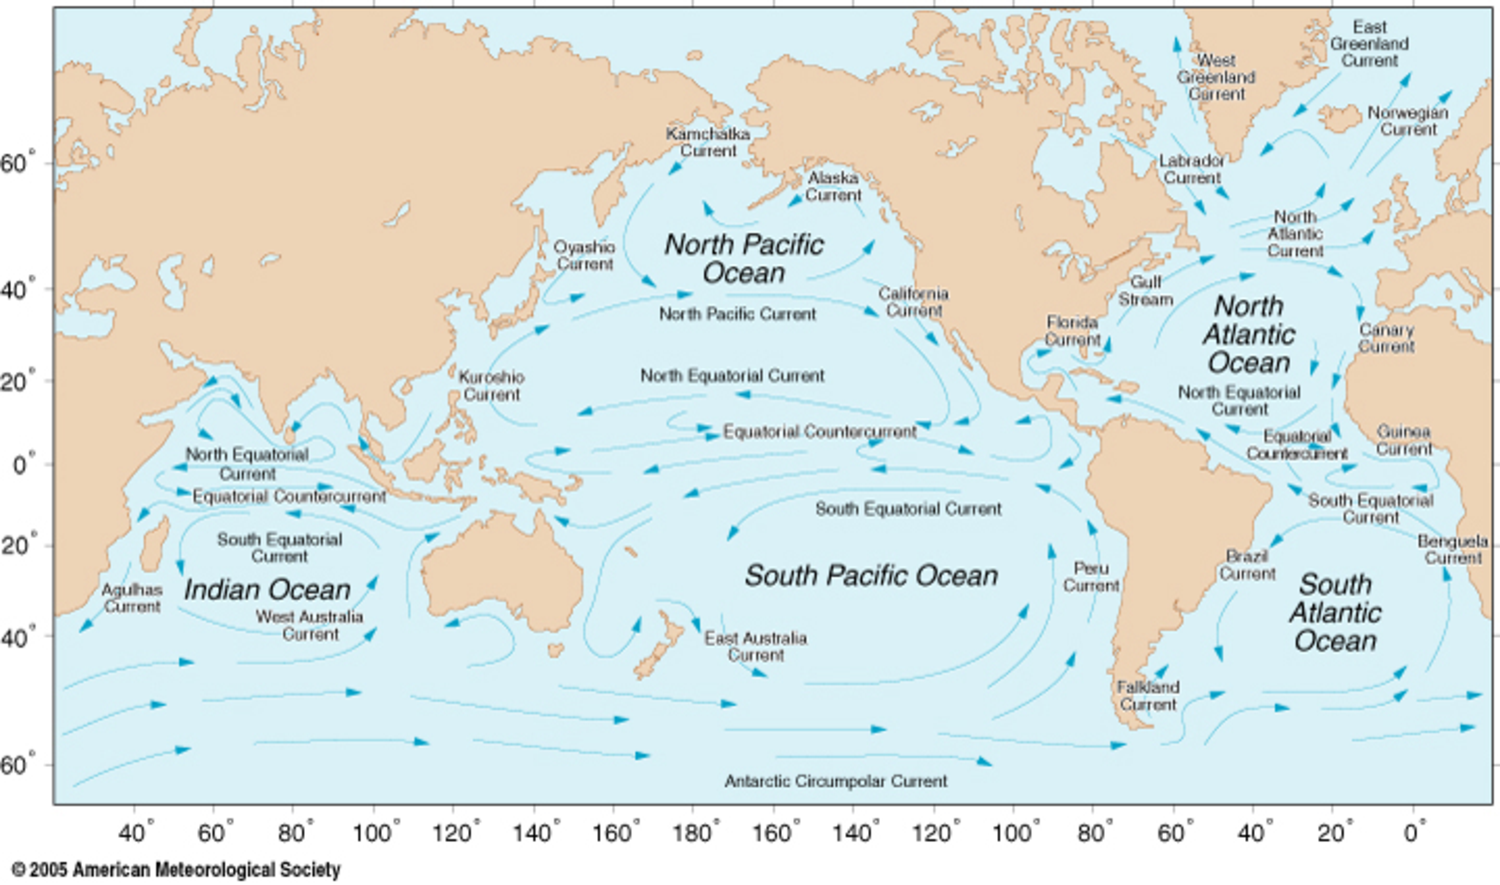
\includegraphics[scale=0.5]{Currents.pdf}
    \caption{Ocean Surface Currents}
    \label{fig:Currents}
  \end{center}
\end{figure}


    \section{A Brief History of Wind-Driven Theory}
    The influence of the coriolis force on the currents of the ocean were first
noted by Hadley, Coriolis, and Ferrel, however the the influence of these forces
were considered too small and therefore didn't show in the theory of the time
\cite{Ekman1905}. Ekman's adviser Bjerknes was the first to indicate the
importance of the influence of the Earth's rotation in the thoery of motions of
the ocean \cite{Ekman1905}. While the true importance of the influence of the
Coriolis force was first noted by the Norwegian scientist Fridtjof Nansen
\cite{Beesley2008, Ekman1905}. Nansen designed a vessel named, the \emph{Fram},
with the intent of allowing it to freeze in the polar ice, and in 1898 Nansen
observed the drift of the \emph{Fram} from its original location. As the vessel
drifted Nansen noticed that the drift was always $20^\circ - 40^\circ$ to the
right of the wind current \cite{Beesley2008}.

\begin{wrapfigure}[9]{l}{0.5\textwidth}
  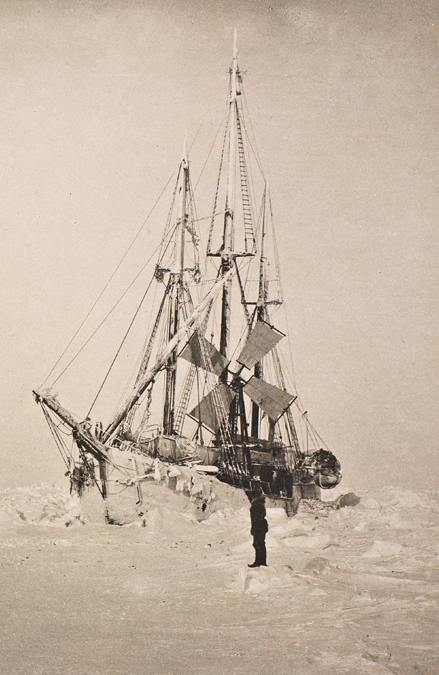
\includegraphics[scale=0.35]{Figures/Fram.jpg}
  \caption{The \emph{Fram} caught in ice in January 1895. Image courtesy of
  FramMuseum.no}
  \label{fig:Fram}
\end{wrapfigure}
In 1905 Ekman\cite{Ekman1905} took the observations made by Nansen and developed
what is considered to be the origin of modern theories for wind-driven ocean
circulation and their effects on ocean currents \cite{Price1987}. According to
Ekman theory momentum from the wind is transferred at the surface of the ocean
to the water, as it blows accross the ocean surface, via wind stress. Then the
Earth's rotation imparts a Coriolis acceleration on the moving water which
causes a deflection of the transport to the right of the surface wind stress in
the Northern Hemisphere and to the left of the surface wind stress in the
Southern Hemisphere \cite{Beesley2008}.

Rossby in his 1936 paper\cite{Rossby1936} introduced a force which he says had
been ``completely disregarded by theoretical investigators although its
existence has been admitted implicitly by practically everyone who has approaced
physical oceanography from the descriptive side.'' The force that Rossby
introduced was the frictional force resulting from large-scale horizontal
mixing. According to Rossby, ``The introduction of this force permits us to see
how motion generated in the surface layers may be diffused and finally
dissipated without recourse to doubtful frictional forces at the bottom of the
ocean.'' Additionally, a significant contribution of Rossby was that he noticed
one could represent the Coriolis force by \cite{James2009}
\begin{equation}
  f = f_0 + \beta\, y,
  \label{eqn:CoriolisParameterization}
\end{equation}
where $f,\, f_0,\, \beta,\, y$ are the Coriolis parameter, reference Coriolis
parameter, $\beta$ is the $\beta$-plane parameter, and $y$ is the $y$-coordinate
(oriented northward), respectively.

Then Sverdrup introduced the idea of a variable \emph{Coriolis parameter}
\cite{Fox-Kemper2003}. By allowing for the variation of the Coriolis parameter
in the north-south direction Sverdrup\cite{Sverdrup1947} introduced, for the
first time, a north-south asymmetry of the problem domain. The term he
introduced, $\nabla \cdot (\mathbf{x} \psi)$ is known as the $\beta$-term
because of the typical notation for the derivative of the Coriolis parameter
\cite{Fox-Kemper2003}. This asymmetry in the north-south direction accounted for
the heretofore unexplained equatorial countercurrents.

Ekman's theory explain the deflection of ocean currents from the direction of
the wind stress and Sverdrup's allowed for an asymmetry in the north-south
direction, thereby resolving the matter of equatorial contercurrents, however,
the combination of the two was still not able to explain the existence of strong
western boundary currents \cite{Fox-Kemper2003}.  Next,
Stommel\cite{Stommel1948} noticed that taken the gradient of the Coriolis term
introduced an asymetry in not only the north-south direction, but also in the
east-west direction. This new term, $\dfrac{\partial \psi}{\partial x}$, which
involves the streamfunction $\psi$ introduces an asymmety in the east-west
direction. This can be seen by substituting $-x$ for $x$-- cleary the sign of
the $\beta$-term changes. This $\beta$-term is a convective term resulting from
the rotation of the Earth. The model developed by Stommel was a simple model
which included the $\beta$-term, a bottom friction term ($-\delta_S \nabla^2
\psi$), and a wind stress forcing term ($F$).  The resultant equation
is \cite{Fox-Kemper2003,Stommel1948,Vallis06}
\begin{equation} \frac{\partial
  \psi}{\partial x} = F - \delta_S \nabla^2 \psi.
  \label{eqn:StommelModel}
\end{equation}
Stommel noted that without the $\beta$-term the solution would be
symmetric in the east-west direction and therefore no western boundary current
would exist \cite{Stommel1948}.

Soon after Stommel's 1948 paper, Munk\cite{Munk1950} published a paper on the
westward intensification of ocean currents. In his paper, Munk explains that
``[i]n Ekman's and Stommel's model the ocean is assumed homogeneous, a case
which the currents extend to the very bottom.'' Munk points out that this is
``in contrast with observations'' and resulted in ``very difficult'' analysis
for Ekman while Stommel was forced ``to resort to a rather arbitrary frictional
force along the bottom.'' To address this Munk introduces lateral friction with
a constant viscosity. Thus, the Munk problem is
\cite{Fox-Kemper2003,Munk1950,Vallis06}
\begin{equation}
  \frac{\partial \psi}{\partial x} = \delta_M^3\, \Delta^2 \psi + F,
  \label{eqn:MunkProblem}
\end{equation}
where $\delta_m$ is the Munk scale. In addition to the introduction of lateral
viscosity, the Munk problem introduced a fourth-order operator (the Biharmonic
operator), which required an extra boundary condition.  In Munk's 1950
paper\cite{Munk1950}, he used the same boundary conditions that we will
consider, i.e. $\dfrac{\partial \psi}{\partial \mathbf{n}} = 0$.

In 1948 Charney\cite{Charney1948} introduced the quasi-geostrophic
approximation, which relied on the assumption that the Rossby number
\begin{equation}
  Ro = \frac{U}{f\, L},
  \label{eqn:RossbyNumber}
\end{equation}
where $U,\, L$ are the characteristic velocity and length, respectively, was
much much smaller than one.
{\color{red} Finish discussion on Charney's contribution.}

    \section{Problem Overview}
    With the continuous increase in computational power, complex mathematical models
are becoming more and more popular in the numerical simulation of oceanic and
atmospheric flows. For some geophysical flows in which computational efficiency
is of paramount importance, however, simplified mathematical models are central.
For example, the \emph{quasi-geostrophic equations (QGE)}, a standard
mathematical model for large scale oceanic and atmospheric flows
\cite{Cushman11,Majda,Pedlosky92,Vallis06}, are often used in climate modeling
\cite{Dijkstra05}.

The QGE are usually discretized in space by using the \emph{finite difference
method} (FDM) \cite{San11}. The \emph{finite element method} (FEM), however,
offers several advantages over the popular FDM, as outlined in \cite{Myers}: (i)
an easy treatment of complex boundaries, such as those of continents for the
ocean, or mountains for the atmosphere; (ii) an easy grid refinement to achieve
a high resolution in regions of interest \cite{Cascon}; (iii) a natural
treatment of boundary conditions; and (iv) a straightforward approach for the
treatment of multiply connected domains \cite{Myers}. Despite these advantages,
there are relatively few papers that consider the FEM applied to the QGE (see
for example: \cite{Cascon, Fix, LeProvost94, Myers, Stevens82}).

To our knowledge, \emph{all} the finite element (FE) discretizations of the QGE
have been developed for the streamfunction-vorticity formulation, none using the
streamfunction formulation. The reason is simple: The streamfunction-vorticity
formulation yields a second order \emph{partial differential equation (PDE)},
whereas the streamfunction formulation yields a fourth order PDE. Thus, although
the streamfunction-vorticity formulation has two variables ($q$ and $\psi$) and
the streamfunction formulation has just one ($\psi$), the former is the
preferred formulation used in practical computations, since its conforming FE
discretization requires low-order ($C^0$) elements, whereas the latter requires
a high-order ($C^1$) FE discretization.

The streamfunction formulation is, from both mathematical and computational
points of view, completely different from the vorticity-streamfunction
formulation. Indeed, the FE discretization of the streamfunction formulation
generally requires the use of $C^1$ elements (for a conforming discretization),
which makes their implementation challenging. From a mathematical point of view,
however, the streamfunction formulation has the following significant advantage
over the vorticity-streamfunction formulation: there are optimal error estimates
for the FE discretization of the streamfunction formulation (see the error
estimate (13.5) and Table 13.1 in \cite{Gunzburger89}), whereas the available
error estimates for the vorticity-streamfunction formulation are suboptimal.

Despite the simplification made in formulating the QGE from the full-fledged
equations of ocean, the numerical simulation of the QGE is still computationally
challenging when integrating over long time periods, as is the case in climate
modeling. Therefore, it is necessary to reduce the computational cost of QGE
simulations. We will consider the \emph{Two-Level} method for reducing this
computational cost. To our knowledge it will be the first time this approach has
been applied to the streamfunction formulation of the QGE.

Two-level finite element discretizations are very promising approaches for
finite element discretizations of nonlinear partial differential equations
\cite{Fairag98,Layton93}. Two-level finite element discretizations aim to
solve a particular nonlinear elliptic equation by first solving the system on a
coarse mesh and then using the coarse mesh solution as a linearized variable to
solve the linearized elliptic equation on  a fine mesh. The attraction of such a
method is that one need only solve the nonlinear equations on a coarse mesh and
then use this solution to solve on a fine mesh, thereby reducing computational
time without sacrificing much in the way of solution accuracy. The development
of the two-level finite element discretization was originally used by Xu in
\cite{Xu94} and later algorithms for the Navier-Stokes Equations (NSE) were
developed by Layton \cite{Layton93}, Fairag \cite{Fairag98, Fairag03}, and Shao
\cite{Shao11}.

The goals of this paper are five-fold. First, we use a $C^1$ finite element (the
Argyris element) to discretize the streamfunction formulation of the QGE. To the
best of our knowledge, this is the \emph{first} time that a $C^1$ finite element
has been used in the numerical discretization of the QGE. Second, we derive
optimal error estimates for the FE discretization of the QGE and present
supporting numerical experiments. To the best of our knowledge, this is the
first time that optimal error estimates for the QGE have been derived.  Third,
we present a Two-Level algorithm for solving the streamfunction formulation of
the QGE and present the error analysis associated with this algorithm. To the
best of our knowledge, this is the \emph{first} time that such an algorithm has
been applied the the streamfunction formulation of the QGE.  Fourth, we will
present an LES closure model for the streamfunction formulation of the QGE and
its theoretical framework.

    \section{Existing Research}
    Although the FE discretization of the QGE is relatively scarce, the
corresponding error analysis seems to be even more scarce. To our knowledge,
\emph{all} the error analysis for the FE discretization of the QGE has been
done for the vorticity-streamfunction formulation, none being done for the
streamfunction formulation. Furthermore, to the best of our knowledge, all the
available error estimates for the FE discretization of the QGE are
\emph{suboptimal}. The first FE error analysis for the FE discretization of
the QGE was carried out by Fix \cite{Fix}, in which suboptimal error estimates
for the vorticity-streamfunction formulation were proved. Indeed, relationships
(4.7) and (4.8) (and the discussion above these) in \cite{Fix} show that the FE
approximations for \emph{both} the potential vorticity (denoted by $\zeta$) and
streamfunction (denoted by $\psi$) consist of piecewise polynomials of degree
$k-1$. At the top of page 381, the author concludes that the error analysis
yields the following estimates:
\begin{eqnarray}
  \| \psi - \psi^h \|_1 &=& O(h^{k-1}), \label{eqn:fix_1} \\
  \| \zeta - \zeta ^h \|_0 &=& O(h^{k-1}) . \label{eqn:fix_2}
\end{eqnarray}
Although the streamfunction error estimate \eqref{eqn:fix_1} appears to be
optimal, the potential vorticity error estimate \eqref{eqn:fix_2} is clearly
suboptimal. Indeed, using piecewise polynomials of degree $k-1$ for the FE
approximation of the vorticity, one would expect an $O(h^k)$ error estimate in
the $L^2$ norm. Medjo \cite{Medjo99, Medjo00} used a FE discretization of the
vorticity-streamfunction formulation and proved error estimates for the time
discretization, but no error estimates for the spatial discretization. Finally,
Cascon et al. \cite{Cascon} proved both \emph{a priori} and \emph{a posteriori}
error estimates for the FE discretization of the \emph{linear Stommel-Munk}
model (see Section~\ref{ch:Tests} for more details). This model, while similar
to the QGE, has one significant difference: the linear Stommel-Munk model is
linear, whereas the QGE is nonlinear.
%Thus, it appears that \emph{no optimal} error estimates for the FE
%discretization of the QGE exist.

We note that the state-of-the-art in the FE error analysis for the QGE seems to
reflect that for the \emph{two-dimensional Navier-Stokes equations (2D NSE)}, to
which the QGE are similar in form.  Indeed, as carefully discussed in
\cite{Gunzburger89}, the 2D NSE in streamfunction-vorticity formulation are easy
to implement (only $C^0$ elements are needed for a conforming discretization),
but the available error estimates are suboptimal (see Section 11.6 in
\cite{Gunzburger89}).
\begin{remark}
  It must be noted that althought QGE and NSE look quite similar in their
  streamfunction forms, they are quite different. A significant difference lies
  in the asymmetry introduced by the $\beta$-term, $\dfrac{\partial
  \psi}{\partial x}$. This $\beta$-term introduces the effect of the Coriolis
  force and differentiates the western boundary from the eastern boundary.
  As the Rossby number, $Ro$ decreases the affect of the Coriollis becomes more
  and more significant. As can be seen in \autoref{fig:NSEnotQGE} the stronger
  the Coriolis force (smaller $Ro$) the narrower the western boundary layer
  becomes. Additionally, we see that in the two gyre forcing seen in
  \autoref{fig:NSEnotQGE} as $Ro$ decreases the distance between the gyres
  becomes less, creating an internal boundary layer. Both these facts lend to
  precautions that must be taken into account when implementing the QGE, which
  are not necessary in the implementation of the NSE.
  %Thus, stabilization methods for the NSE may not work as well for the QGE.
\end{remark}

\begin{figure}
  \begin{center}
  \begin{subfigure}{0.4\textwidth}
    \centering
    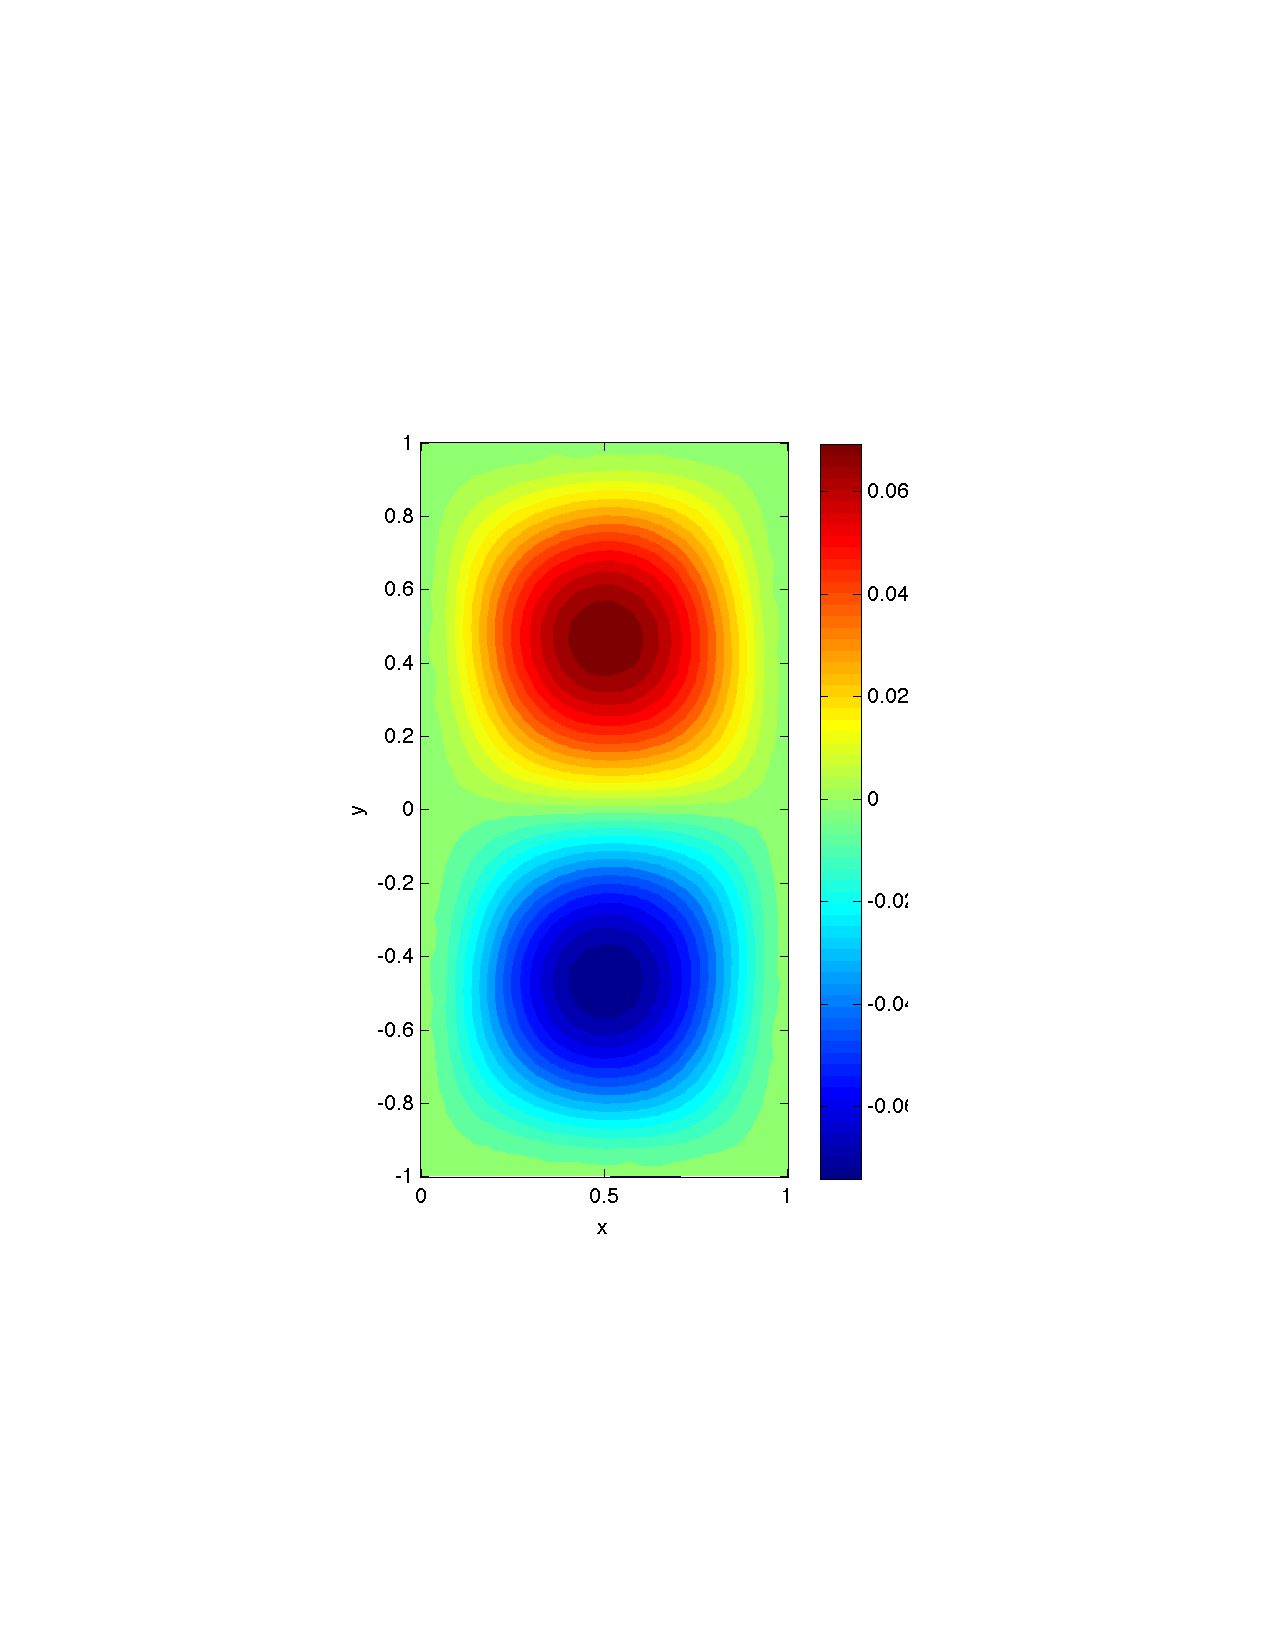
\includegraphics[scale=0.5]{Figures/Re200h16k1000}
    \caption{NSE}
    \label{sfi:NSE}
  \end{subfigure}
  \begin{subfigure}{0.4\textwidth}
    \centering
    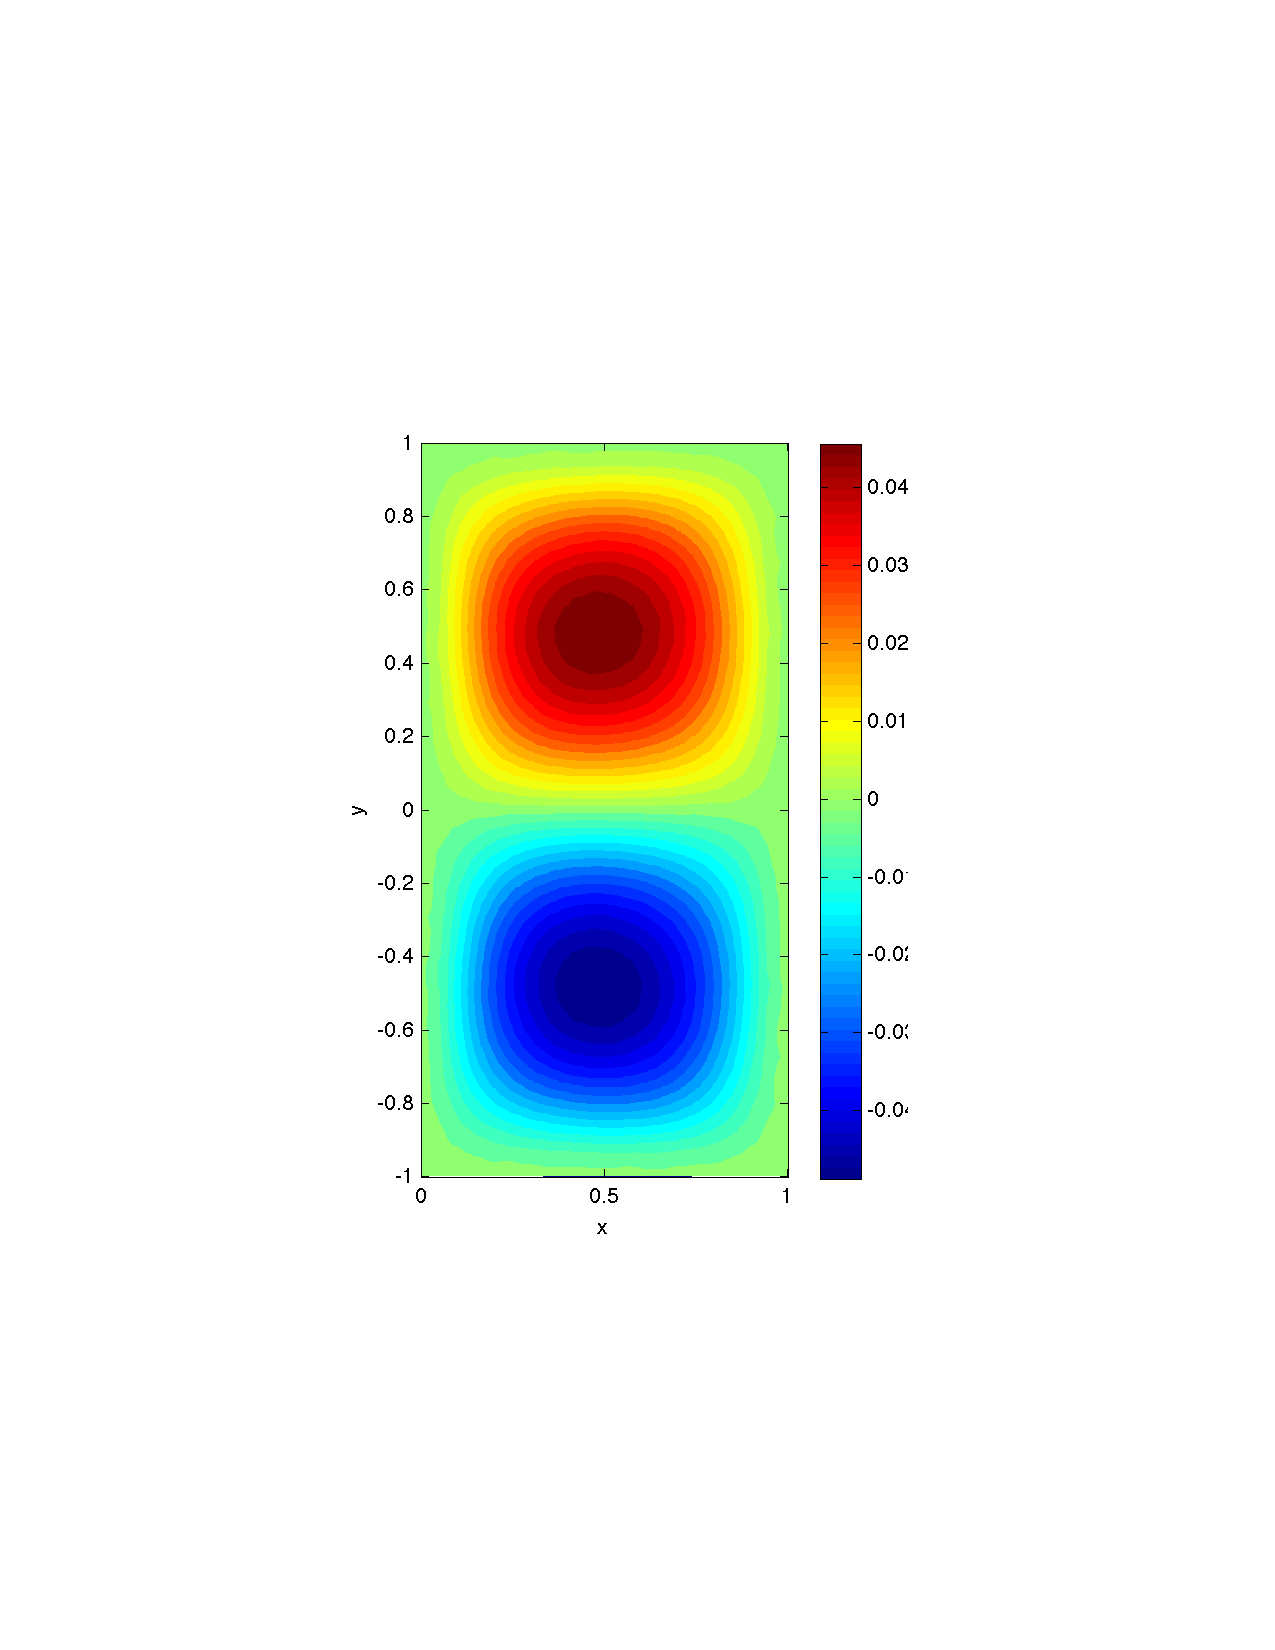
\includegraphics[scale=0.5]{Figures/Re200Ro1h16k1000}
    \caption{$Ro=1$}
    \label{sfi:QGERo1}
  \end{subfigure}
  \begin{subfigure}{0.3\textwidth}
    \centering
    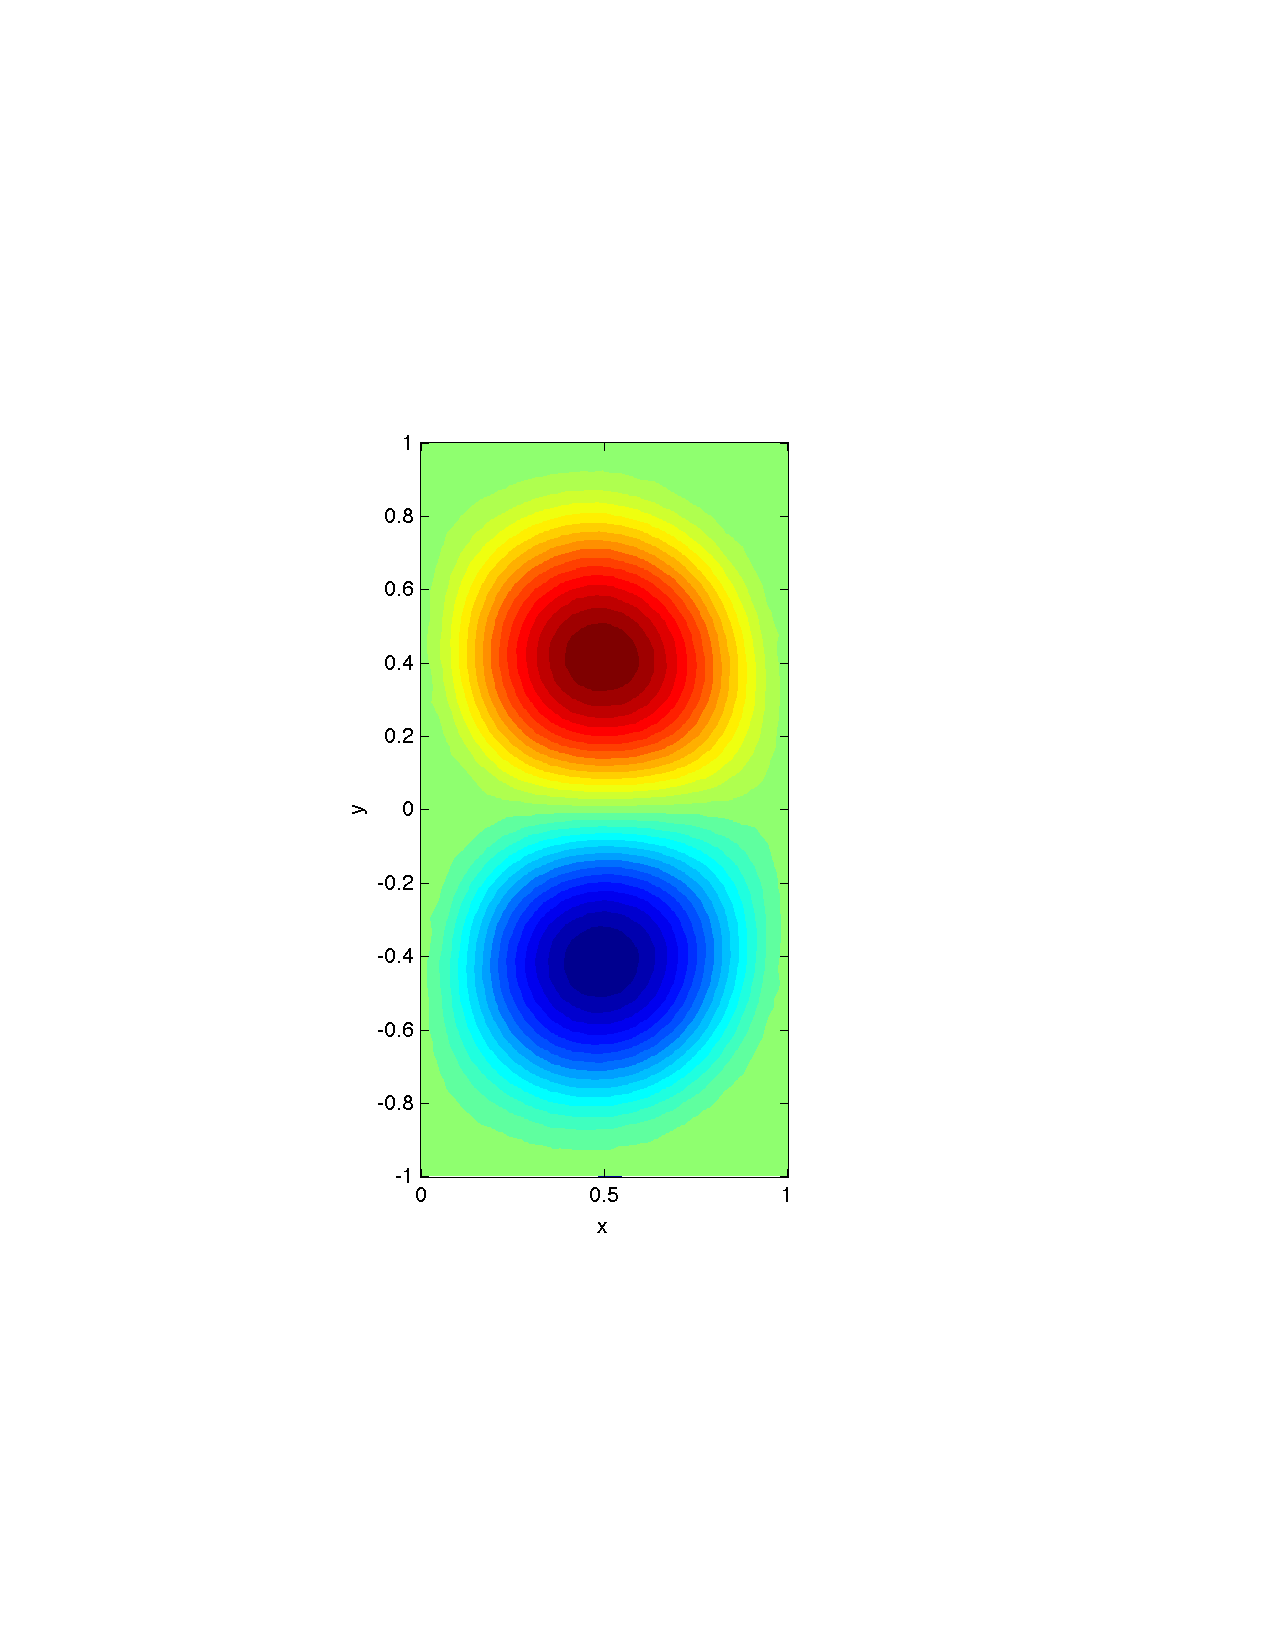
\includegraphics[scale=0.5]{Figures/Re200Ro1E-1h16k1000}
    \caption{$Ro=0.1$}
    \label{sfi:QGERo0.1}
  \end{subfigure}
  \begin{subfigure}{0.3\textwidth}
    \vspace{1.3em}
    \centering
    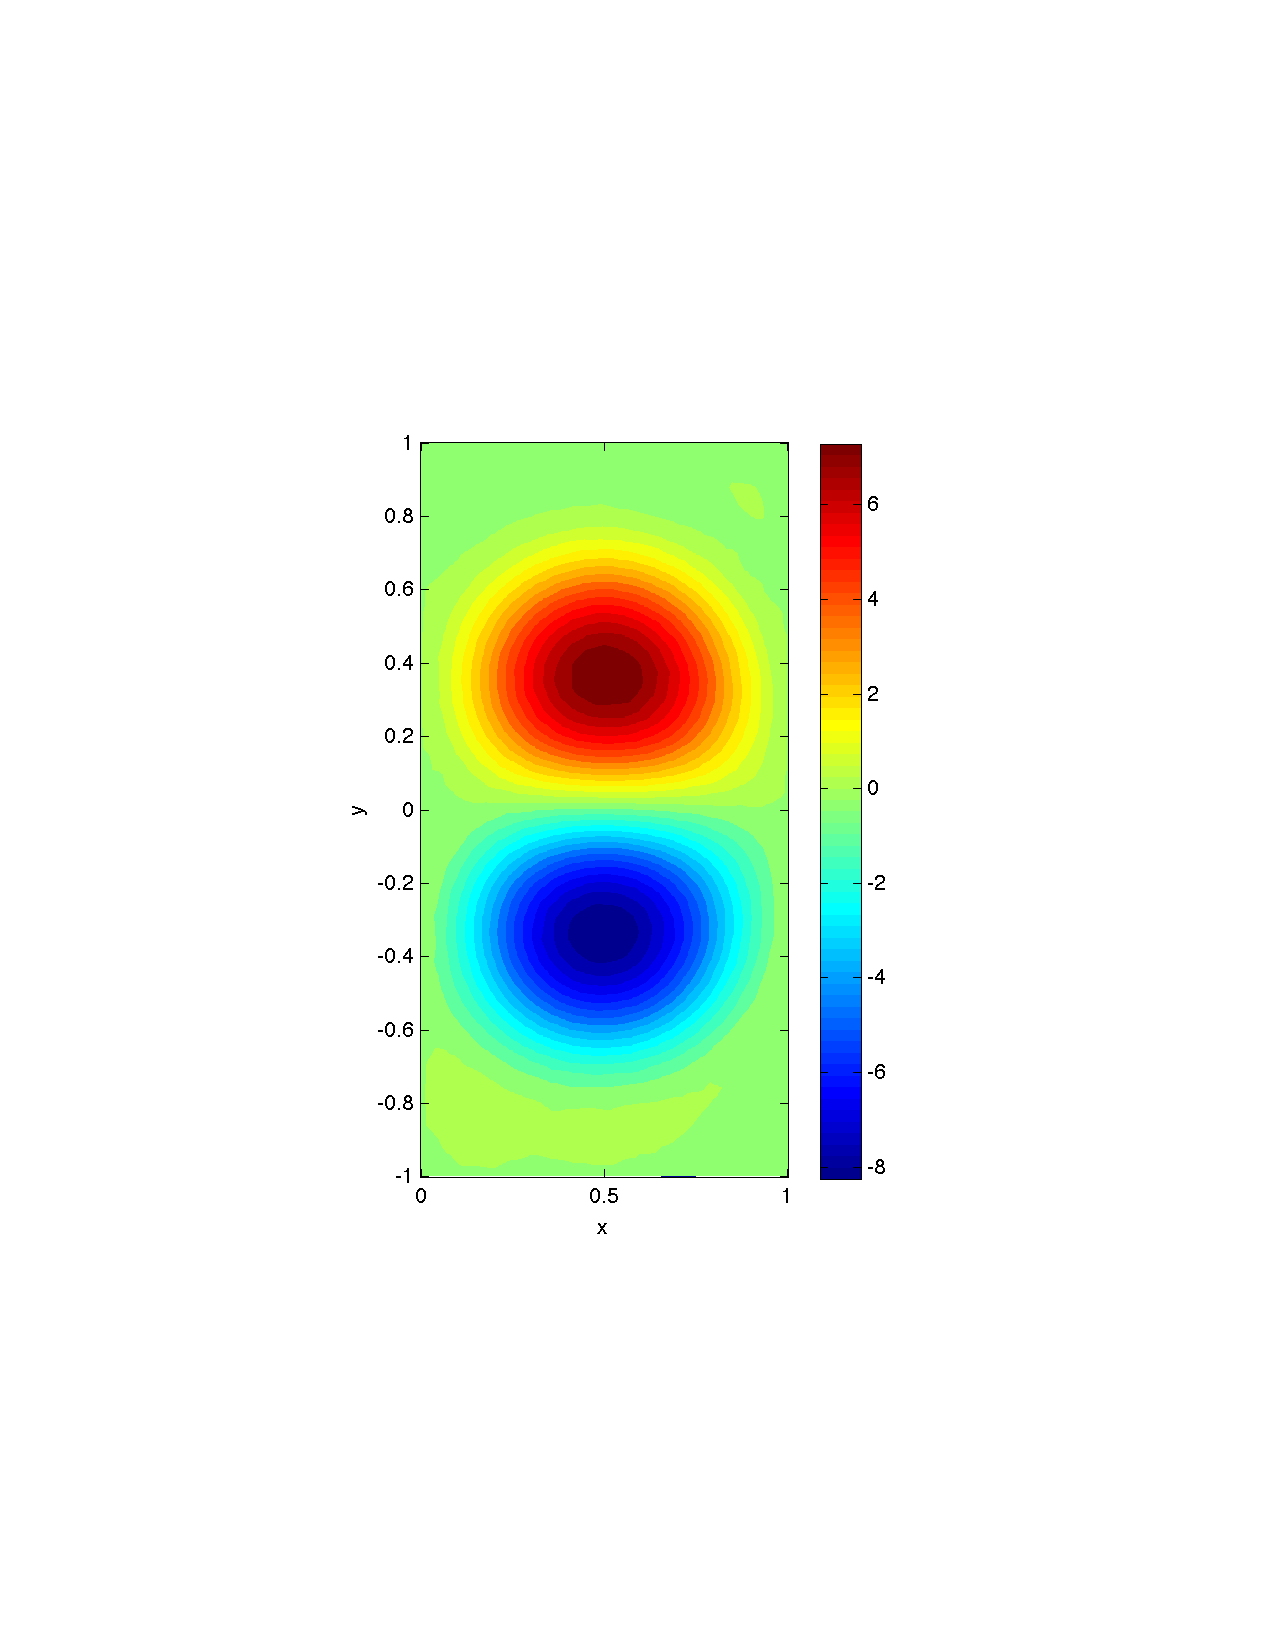
\includegraphics[scale=0.5]{Figures/Re200Ro1E-2h16k1000}
    \label{sfi:QGERo0.01}
    \caption{$Ro=0.01$}
  \end{subfigure}
  \begin{subfigure}{0.3\textwidth}
    \centering
    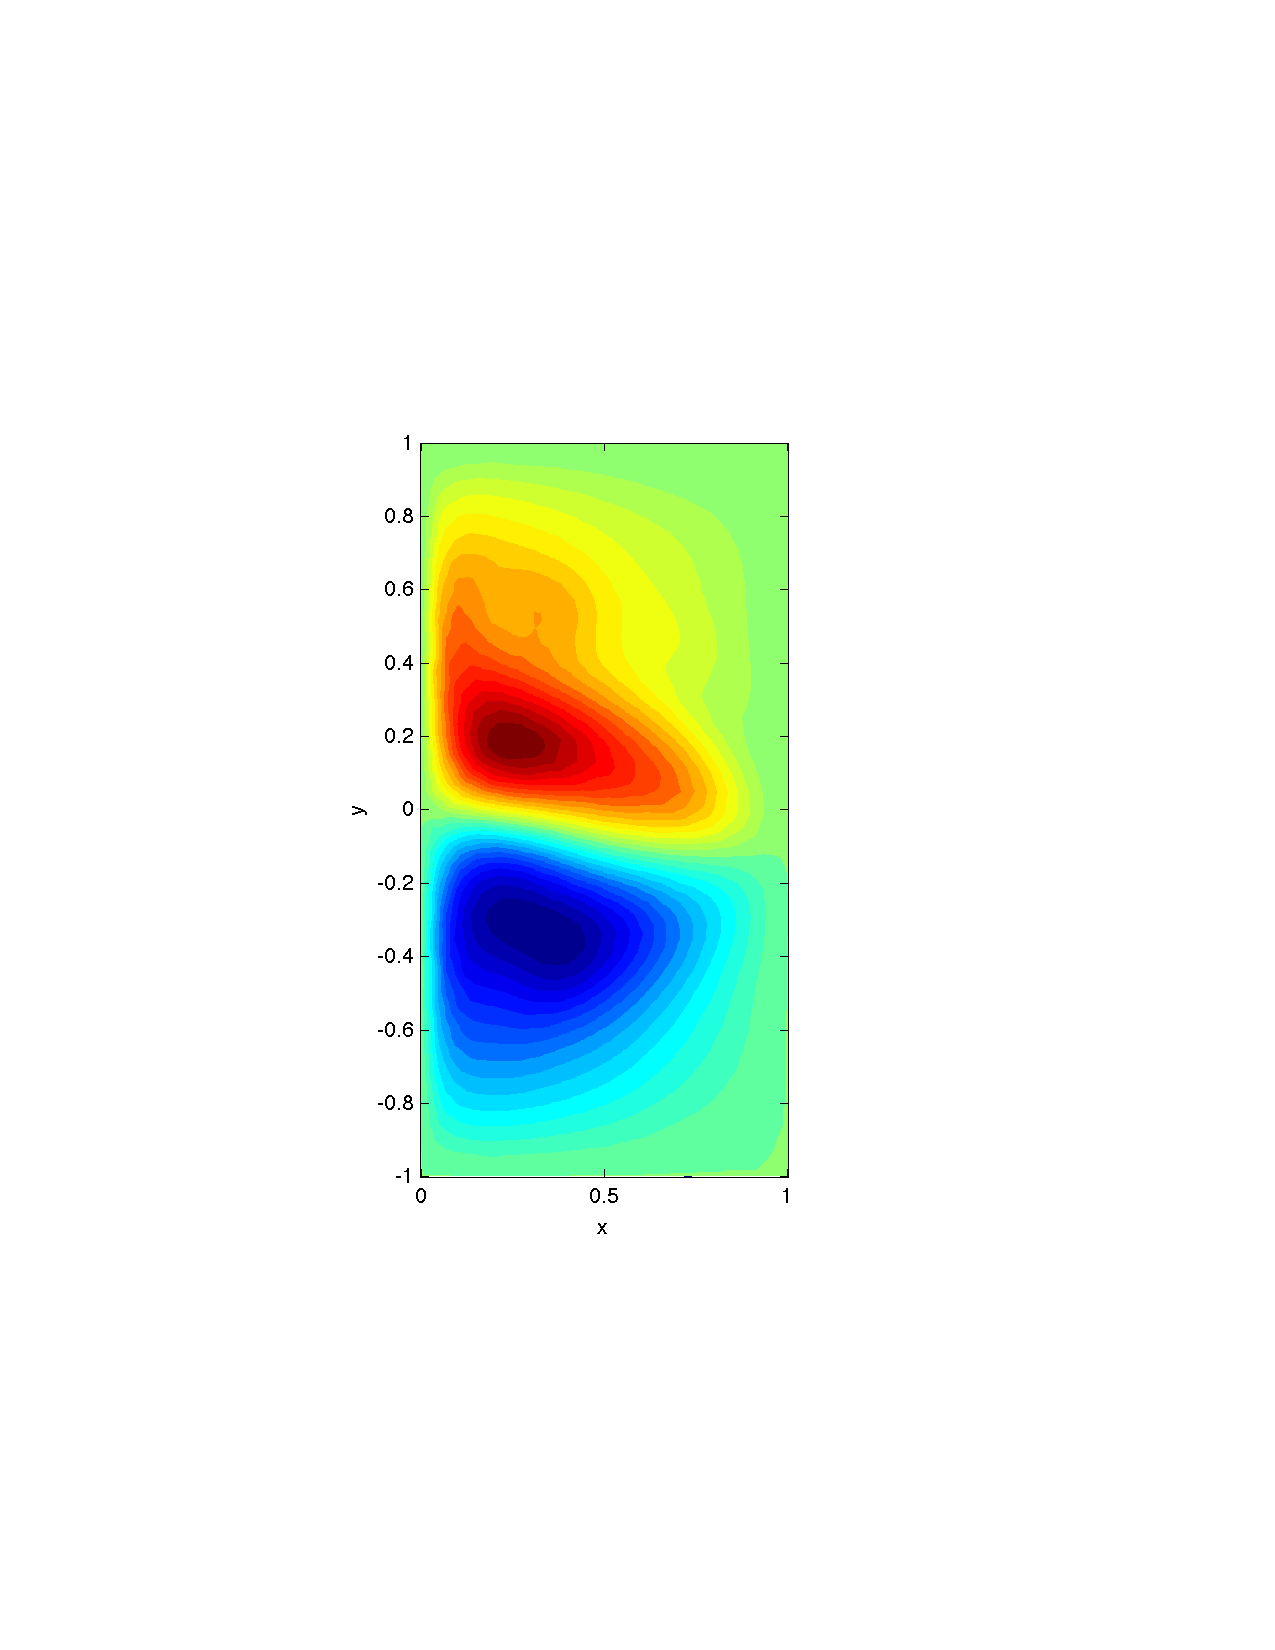
\includegraphics[scale=0.5]{Figures/Re200Ro1E-3h16k1000}
    \caption{$Ro=0.001$}
    \label{sfi:QGERo0.001}
  \end{subfigure}
  \caption{QGE is not NSE: Time Averaged, $t=\lbrack 0, 10\rbrack,\, dt=1\times
    10^{-3},\, Re= 200,\, F = \sin \pi y$.}
  \label{fig:NSEnotQGE}
  \end{center}
\end{figure}

Next, we summarize the discussion in \cite{Gunzburger89},
since we believe it sheds light on the QGE setting. For $C^0$ piecewise
polynomial of degree $k$ FE approximation for \emph{both} the vorticity
(denoted by $\omega$) and streamfunction (denoted by $\psi$), the error
estimates given in \cite{Girault86} are (see (1.26) in \cite{Gunzburger89}):
\begin{eqnarray}
  | \psi - \psi^h |_1 + \| \omega - \omega^h \|_0 \leq C \, h^{k - 1/2} \, | \ln h |^{\sigma} ,
  \label{eqn:gunzburger_1}
\end{eqnarray}
where $\sigma = 1$ for $k = 1$ and $\sigma = 0$ for $k > 1$. It is noted in
\cite{Gunzburger89} that the error estimate in \eqref{eqn:gunzburger_1} is not
optimal: one may loose a half power in $h$ for the derivatives of the
streamfunction (i.e., for the velocity), and three-halves power for the
vorticity. It is also noted that there is computational and theoretical evidence
that \eqref{eqn:gunzburger_1} is not sharp with respect to the streamfunction
error. Furthermore, in \cite{Fix84} it was shown that, for the \emph{linear}
Stokes equations, the derivatives of the streamfunction are essentially
optimally approximated (see (11.27) in \cite{Gunzburger89}):
\begin{eqnarray}
  | \psi - \psi^h |_1 \leq C \, h^{k - \varepsilon} , \label{eqn:gunzburger_2}
\end{eqnarray}
where $\varepsilon = 0$ for $k > 1$ and $\varepsilon > 0$ is arbitrary for $k =
1$. That being said, it is then noted in \cite{Gunzburger89} that
\eqref{eqn:gunzburger_1} seems to be sharp for the vorticity error and thus
vorticity approximations are, in general, very poor.

    \section{Outline}
    The rest of the paper is organized as follows: \autoref{sec:QGE} presents the
QGE, and \autoref{sec:SQGE} presents the stationary QGE. Then
\autoref{ch:WellPosed} discusses the mathematical framework of both the QGE
and SQGE.  In \autoref{ch:FEM} we outline the FE discretization for the QGE
(\autoref{sec:QGEFEM}), and SQGE (\autoref{sec:SQGEFEM}), with special emphasis
placed on the Argyris element in \autoref{sec:Argyris}. Additionally, a discussion
of the two-level method is presented in \autoref{sec:TwoLevel}. Rigorous error
estimates for the FE discretization of the SQGE, the two-level method applied
to the SQGE, and the QGE are derived in \autoref{sec:SQGEErrors},
\autoref{sse:SQGE2LE}, and \autoref{sec:QGEError}, respectively.  Several
numerical experiments supporting the theoretical results for the QGE, SQGE and
the two-level method are presented in \autoref{sec:QGETests},
\autoref{sec:SQGETests}, and \autoref{sec:SQGE2LTests}. These numerical
experiments also tackle geophysical flows in realistic complex geometries with
realistic parameter values. Finally, conclusions are included in
\autoref{ch:Conclusions}.



  \chapter{Governing Equations} \label{ch:Model}
  One of the most popular mathematical models used in the study of large scale
wind-driven ocean circulation is the QGE \cite{Cushman11,Vallis06}. The QGE
represent a simplified model of the full-fledged equations (e.g., the Boussinesq
equations), which allows efficient numerical simulations while preserving many
of the essential features of the underlying large scale ocean flows. The
assumptions used in the derivation of the QGE include the hydrostatic balance,
the $\beta$-plane approximation, the geostrophic balance, and the eddy viscosity
parametrization.  Details of the derivation of the QGE and the approximations
used along the way can be found in standard textbooks on geophysical fluid
dynamics, such as
\cite{Cushman11,Majda,Majda03,McWilliams06,Pedlosky92,Vallis06}.

In the \emph{one-layer QGE}, sometimes called the barotropic vorticity equation,
the flow is assumed to be homogenous in the vertical direction. Thus,
stratification effects are ignored in this model.  The practical advantages of
such a choice are obvious: the computations are two-dimensional, and, thus, the
corresponding numerical simulation have a low computational cost. To include
stratification effects, QGE models of increasing complexity have been devised by
increasing the number of layers in the model (e.g., the two-layer QGE and the
$N$-layer QGE \cite{Vallis06}). As a first step, in this report we use the
one-layer QGE (referred to as ``the QGE" in what follows) to study the
wind-driven circulation in an enclosed, midlatitude rectangular basin, which is
a standard problem, studied extensively by modelers \cite{Cushman11, Layton08,
Majda03, Majda, McWilliams06, Vallis06, Pedlosky92}.


    \section{The Quasi-Geostrophic Equations} \label{sec:QGE}
    One of the most popular mathematical models used in the study of large scale
wind-driven ocean circulation is the QGE \cite{Cushman11,Vallis06}. The QGE
represent a simplified model of the full-fledged equations (e.g., the Boussinesq
equations), which allows efficient numerical simulations while preserving many
of the essential features of the underlying large scale ocean flows. The
assumptions used in the derivation of the QGE include the hydrostatic balance,
the $\beta$-plane approximation, the geostrophic balance, and the eddy viscosity
parametrization.  Details of the derivation of the QGE and the approximations
used along the way can be found in standard textbooks on geophysical fluid
dynamics, such as
\cite{Cushman11,Majda,Majda03,McWilliams06,Pedlosky92,Vallis06}.

In the \emph{one-layer QGE}, sometimes called the barotropic vorticity equation,
the flow is assumed to be homogenous in the vertical direction. Thus,
stratification effects are ignored in this model.  The practical advantages of
such a choice are obvious: the computations are two-dimensional, and, thus, the
corresponding numerical simulation have a low computational cost. To include
stratification effects, QGE models of increasing complexity have been devised by
increasing the number of layers in the model (e.g., the two-layer QGE and the
$N$-layer QGE \cite{Vallis06}). As a first step, in this report we use the
one-layer QGE (referred to as ``the QGE" in what follows) to study the
wind-driven circulation in an enclosed, midlatitude rectangular basin, which is
a standard problem, studied extensively by modelers \cite{Cushman11, Layton08,
Majda03, Majda, McWilliams06, Vallis06, Pedlosky92}.

The QGE are usually written as follows (see, e.g., equation (14.57) in
\cite{Vallis06}, equation (1.1) in \cite{Majda}, equation (1.1) in
\cite{Wang94}, and equation (1) in \cite{Greatbatch00}):
\begin{align}
  \frac{\partial q}{\partial t} + J(\psi , q) &= A \, \Delta q + F
    \label{qge_q_psi_dim_1} \\
  q &= \Delta \psi + \beta \, y , \label{qge_q_psi_dim_2}
\end{align}
where $q$ is the potential vorticity, $\psi$ is the velocity streamfunction,
$\beta$ is the coefficient multiplying the $y$ coordinate (which is oriented
northward) in the $\beta$-plane approximation \eqref{eqn:beta_plane}, $F$ is the
forcing, $A$ is the eddy viscosity parametrization, and $J(\cdot , \cdot)$ is
the Jacobian operator given by
\begin{align}
  J(\psi , q) := \frac{\partial \psi}{\partial x} \, \frac{\partial q}{\partial y} -
    \frac{\partial \psi}{\partial y} \, \frac{\partial q}{\partial x} . \label{eqn:jacobian}
\end{align}
The $\beta$-plane approximation reads
\begin{align}
  f = f_0 + \beta \, y , \label{eqn:beta_plane}
\end{align}
where $f$ is the Coriolis parameter and $f_0$ is the reference Coriolis
parameter (see, e.g., the discussion on page 84 in \cite{Cushman94} or Section
2.3.2 in \cite{Vallis06}).

As noted in Chapter 10.7.2 in \cite{Vallis06} (see also \cite{San12}), the eddy
viscosity parameter $A$ in \eqref{qge_q_psi_dim_1} is usually several orders of
magnitude higher than the molecular viscosity. This choice allows the use of a
coarse mesh in numerical simulations. The horizontal velocity $\mathbf{u}$ can
be recovered from $\psi$ and $q$ by using the following formula:
\begin{align}
  \mathbf{u} := \nabla^{\perp} \psi =
    \begin{pmatrix} - \frac{\partial \psi}{\partial y} \\
    \frac{\partial \psi}{\partial x}
  \end{pmatrix} .
\label{eqn:u_psi}
\end{align}

The computational domain is standard \cite{Greatbatch00}, a rectangular, closed
basin on a $\beta$-plane with the $y$ coordinate increasing northward and the
$x$ coordinate eastward. The center of the basin is at $y=0$, the northern and
southern boundaries are at $y = \pm \, L$, respectively, and the western and
eastern boundaries are at $x = 0$ and $x = L$ (see Figure 1 in
\cite{Greatbatch00}).

We are now ready to nondimensionalize the QGE
\eqref{qge_q_psi_dim_1}-\eqref{qge_q_psi_dim_2}.  There are several ways of
nondimensionalizing the QGE, based on different scalings and involving different
parameters (see standard textbooks, such as
\cite{Cushman11,Majda,Pedlosky92,Vallis06}).  Since the FEM error analysis in
this report is based on a precise relationship among the nondimensional
parameters of the QGE (see, e.g., \eqref{eqn:small_data_condition}), we present
below a careful nondimensionalization of the QGE.

We first need to choose a length scale and a velocity scale. The length scale we
choose is $L$, the width of the computational domain. The velocity scale is the
Sverdrup velocity
\begin{align}
  U := \frac{\pi \, \tau_0}{\rho \, H \, \beta \, L} , \label{eqn:velocity_scale}
\end{align}
where $\tau_0$ is the amplitude of the wind stress, $\rho$ is the density of the
fluid, and $H$ is the height of the fluid. The Sverdrup balance, which was used
in the derivation of \eqref{eqn:velocity_scale}, expresses the balance between
the two dominant effects in the system: the $\beta$-effect and the curl of the
divergence of the wind stress (see, e.g., Section 14.1.3 in \cite{Vallis06}).
Once the length and velocity scales are chosen, the variables in the QGE
\eqref{qge_q_psi_dim_1}-\eqref{qge_q_psi_dim_2} can be nondimensionalized as
follows:
\begin{align}
  x^* = \frac{x}{L}, \quad
  y^* = \frac{y}{L}, \quad
  t^* = \frac{t}{L / U}, \quad
  q^* = \frac{q}{\beta \, L}, \quad
  \psi^* = \frac{\psi}{U \, L} ,
\label{eqn:nondimensional_variables}
\end{align}
where a $^*$ superscript denotes the nondimensional variable. We first
nondimensionalize \eqref{qge_q_psi_dim_2}. Using
\eqref{eqn:nondimensional_variables}, \eqref{qge_q_psi_dim_2} becomes
\begin{align}
  \beta \, L \, q^* = \frac{1}{L^2} \, \Delta^* (U \, L \, \psi^*) + \beta \, (L \, y^*) .
  \label{qge_q_psi_nondim_1}
\end{align}
Dividing \eqref{qge_q_psi_nondim_1} by $\beta \, L$, we get:
\begin{align}
  q^* = \left( \frac{U}{\beta \, L^2} \right) \, \Delta^* \psi^* + y^* .
  \label{qge_q_psi_nondim_2}
\end{align}
Defining the \emph{Rossby number $Ro$} as follows
\begin{align}
  Ro := \frac{U}{\beta \, L^2} , \label{eqn:rossby_number}
\end{align}
equation \eqref{qge_q_psi_nondim_2} becomes
\begin{align}
  q^* = Ro \, \Delta^* \psi^* + y^* .
  \label{qge_q_psi_nondim_3}
\end{align}

We note that all the nondimensionalizations in
\eqref{eqn:nondimensional_variables} are naturally based on the velocity scale
$U$ and the length scale $L$, except $q^*$. Indeed, a nondimensionalization of
the form
\begin{align}
  {\tilde q} = \frac{U}{L},
  \label{eqn:qge_q_psi_nondim_4}
\end{align}
would probably be more natural. Note that the alternative nondimensionalization
in \eqref{eqn:qge_q_psi_nondim_4} is indeed correct, i.e., the variable ${\tilde
q}$ is nondimensional.  The main reason for which the nondimensionalization in
\eqref{eqn:nondimensional_variables} is used instead the one in
\eqref{eqn:qge_q_psi_nondim_4} is that the former yields just one constant (the
Rossby number $Ro$) in \eqref{qge_q_psi_nondim_3}, whereas the latter would
yield two constants.

Next, we nondimensionalize \eqref{qge_q_psi_dim_1}. We start with the left-hand
side:
\begin{align}
  \frac{\partial q}{\partial t} &= ( \beta \, U) \, \frac{\partial q^*}{\partial t^*} ,
    \label{eqn:qge_q_psi_nondim_5} \\[0.2cm]
  J(\psi,q) &=  \frac{\partial \psi}{\partial x} \, \frac{\partial q}{\partial y} - \frac{\partial
    \psi}{\partial y} \, \frac{\partial q}{\partial x}
    = U \, \frac{\partial \psi^*}{\partial x^*} \, \beta \, \frac{\partial q^*}{\partial y^*} - U \,
      \frac{\partial \psi^*}{\partial y^*} \,  \beta \, \frac{\partial q^*}{\partial x^*}
      \nonumber \\[0.2cm]
  &= (  \beta \, U ) \, J^*(\psi^*,q^*) .
  \label{eqn:qge_q_psi_nondim_6}
\end{align}

Next, we nondimensionalize the right-hand side of \eqref{qge_q_psi_dim_1}. The
first term can be nondimensionalized as follows:
\begin{align}
  \frac{\partial q}{\partial t} A \, \Delta q &= A \, \left( \frac{\partial^2 q}{\partial x^2} +
    \frac{\partial^2 q}{\partial y^2} \right)
%\nonumber \\[0.2cm]
%&=
    = A \,  \left( \frac{1}{L^2} \, \frac{\partial^2}{\partial {x^*}^2} \, (\beta \, L \, q^*) +
      \frac{1}{L^2} \, \frac{\partial^2}{\partial {y^*}^2} \, (\beta \, L \, q^*) \right) \nonumber
      \\[0.2cm]
  &= A \, \frac{\beta}{L} \, \Delta^* q^* .
  \label{eqn:qge_q_psi_nondim_7}
\end{align}
Thus, inserting \eqref{eqn:qge_q_psi_nondim_5}-\eqref{eqn:qge_q_psi_nondim_7} in
\eqref{qge_q_psi_dim_1}, we get:
\begin{align}
  ( \beta \, U) \, \frac{\partial q^*}{\partial t^*} + (  \beta \, U ) \, J^*(\psi^*,q^*)
  &= A \, \frac{\beta}{L} \, \Delta^* q^* + F .
  \label{eqn:qge_q_psi_nondim_8}
\end{align}
Dividing by $\beta \, U$, we get:
\begin{align}
  \frac{\partial q^*}{\partial t^*} + J^*(\psi^*,q^*) &= \left( \frac{A}{U \, L} \right) \,
    \Delta^* q^* + \frac{F}{\beta \, U} .
\label{eqn:qge_q_psi_nondim_9}
\end{align}
Defining the \emph{Reynolds number $Re$} as follows
\begin{align}
Re
:= \frac{U \, L}{A} ,
\label{eqn:reynolds_number}
\end{align}
equation \eqref{eqn:qge_q_psi_nondim_9} becomes
\begin{align}
  \frac{\partial q^*}{\partial t^*} + J^*(\psi^*,q^*) &= Re^{-1} \, \Delta^* q^*
    + \frac{F}{\beta\, U} .
  \label{eqn:qge_q_psi_nondim_10}
\end{align}
As noted above, the Sverdrup balance expresses the balance between the two
dominant effects in the system: the $\beta$-effect and the curl of the
divergence of the wind stress (see, e.g., Section 14.1.3 in \cite{Vallis06}).
The velocity scale $U$ in \eqref{eqn:velocity_scale} was chosen according to the
Sverdrup balance.  Thus, the last term on the right-hand side of
\eqref{eqn:qge_q_psi_nondim_10} has the following units:
\begin{align}
\left[ \frac{F}{\beta \, U} \right]
\sim \left[ \frac{\frac{\nabla \times (\nabla \cdot \tau_0)}{\rho}}{\beta \, U}  \right]
\stackrel{\eqref{eqn:velocity_scale}}{\sim}
\left[ \frac{\frac{\nabla \times (\nabla \cdot \tau_0)}{\rho}}{\frac{\pi \, \tau_0}{\rho \, H \, L}}  \right] ,
\label{eqn:qge_q_psi_nondim_11}
\end{align}
which, after the obvious simplification, is clearly nondimensional.  Thus,
\eqref{eqn:qge_q_psi_nondim_11} clearly shows that the last term on the
right-hand side of \eqref{eqn:qge_q_psi_nondim_10} is nondimensional, so
\eqref{eqn:qge_q_psi_nondim_10} becomes:
\begin{align}
  \frac{\partial q^*}{\partial t^*} + J^*(\psi^*,q^*)
  &= Re^{-1} \, \Delta^* q^* + F^* .
\label{eqn:qge_q_psi_nondim_12}
\end{align}

Dropping the $^*$ superscript in \eqref{eqn:qge_q_psi_nondim_12}, we obtain the
nondimensional {\it vorticity-streamfunction formulation} of the \emph{one-layer
quasi-geostrophic equations}
\begin{align}
  \frac{\partial q}{\partial t} + J(\psi , q) &= Re^{-1} \, \Delta q + F \label{qge_q_psi_1} \\
  q &= Ro \, \Delta \psi + y, \label{qge_q_psi_2}
\end{align}
where $Re$ and $Ro$ are the Reynolds and Rossby numbers, respectively.

Substituting \eqref{qge_q_psi_2} in \eqref{qge_q_psi_1} and dividing by $Ro$, we
get the {\it streamfunction formulation} of the \emph{one-layer quasi-geostrophic
equations}
\begin{align}
  \frac{\partial \left[ \Delta \psi \right]}{\partial t} - Re^{-1} \, \Delta^2 \psi + J(\psi
    , \Delta \psi) + Ro^{-1} \, \frac{\partial \psi}{\partial x} = Ro^{-1} \, F. \label{qge_psi_1}
\end{align}
Equations \eqref{qge_q_psi_1}-\eqref{qge_q_psi_2} and \eqref{qge_psi_1} are the
usual formulations of the one-layer QGE in streamfunction-vorticity and
streamfunction formulations, respectively. We note that the
streamfunction-vorticity formulation has two unknowns ($q$ and $\psi$), whereas
the streamfunction formulation has only one unknown ($\psi$). The
streamfunction-vorticity formulation, however, is more popular than the
streamfunction formulation, since the former is a second-order PDE, whereas the
latter is a fourth-order PDE.

We also note that \eqref{qge_q_psi_2}-\eqref{qge_q_psi_1} and \eqref{qge_psi_1}
are similar in form to the 2D NSE written in the streamfunction-vorticity and
streamfunction formulations, respectively.  Indeed,
\eqref{qge_q_psi_1}-\eqref{qge_q_psi_2} and \eqref{qge_psi_1} are almost the
same as (11.3)-(11.4) and (13.1) in \cite{Gunzburger89}, which are obtained by
first writing
\begin{align}
  \mathbf{u} = \begin{pmatrix} \frac{\partial \psi}{\partial y} \\[0.2cm]
      - \frac{\partial \psi}{\partial x}
    \end{pmatrix} \label{qge_psi_2}
\end{align}
and then taking the curl of the 2D NSE.

There are, however, several significant differences between the QGE and the 2D
NSE. First, we note that the term $y$ in \eqref{qge_q_psi_2} and the
corresponding term $\dfrac{\partial \psi}{\partial x}$ in \eqref{qge_psi_1},
which model the \emph{rotation effects} in the QGE, do not have counterparts in
the 2D NSE.  Furthermore, the Rossby number, $Ro$, in the QGE, which is a
measure of the rotation effects, does not appear in the 2D NSE.  However, apart
from these two significant differences, the streamfunction-vorticity and
streamfunction formulations of the QGE and the 2D NSE are quite similar.

Thus, for notation consistency (i.e., to ensure that the velocity and the
streamfunction are related by \eqref{qge_psi_2}), we will consider the QGE
\eqref{qge_psi_1} with $\psi$ replaced with $-\psi$:
\begin{align}
  -\frac{\partial \left[ \Delta \psi \right]}{\partial t} + Re^{-1} \, \Delta^2 \psi + J(\psi , \Delta \psi)
    - Ro^{-1} \, \frac{\partial \psi}{\partial x} = Ro^{-1} \, F .  \label{eqn:QGE_psi}
\end{align}

At this point, let us comment on the significance of the two parameters in
\eqref{eqn:QGE_psi}, the Reynolds number $Re$ and the Rossby number $Ro$.  As in
the 2D NSE case, $Re$ is the coefficient of the diffusion term $- \Delta q =
\Delta^2 \psi$.  The higher $Re$, the smaller the magnitude of the diffusion
term as compared with the nonlinear convective term $- J(\psi, \Delta \psi) = (
\nabla \psi^{\perp} \cdot \nabla ) q = (\mathbf{u} \cdot \nabla ) q$.  Since
$Ro$, quantifying the rotation effects in the QGE, does not appear in the 2D
NSE, its significance deserves a special attention.  We first note that, for
small $Ro$, which corresponds to large rotation effects, the forcing term
$Ro^{-1} \, F$ becomes large as compared with the other terms.  But probably the
most interesting term in \eqref{eqn:QGE_psi} is $\displaystyle Ro^{-1} \,
\frac{\partial \psi}{\partial x}$, which could be interpreted as a convection
type term with respect to $\psi$, not to $q = -\Delta \psi$.  When $Ro$ is
small, $\displaystyle Ro^{-1} \, \frac{\partial \psi}{\partial x}$ becomes
large.  In conclusion, the physically relevant cases for large scale oceanic
flows, in which $Re$ is large and $Ro$ is small (i.e., small diffusion and high
rotation, respectively) translate mathematically into a
\emph{convection-dominated} PDE with \emph{large forcing}.  Thus, from a
mathematical point of view, we expect the restrictive conditions used to prove
the well-posedness of the 2D NSE \cite{Girault79,Girault86,Gunzburger89} will be
even more restrictive in the QGE setting, due to the rotation effects.  We will
later see that this is indeed the case.

To completely specify the equations in \eqref{eqn:QGE_psi}, we need to impose
boundary conditions.  The question of appropriate boundary conditions for the
QGE is a thorny one, especially for the vorticity-streamfunction formulation
(see \cite{Vallis06,Cummins} for a careful discussion of this issue).  In this
report, we consider
\begin{equation}
  \begin{split}
    \psi = \frac{\partial \psi}{\partial \mathbf{n}} = 0 \qquad \text{on } \partial \Omega, \\
    \psi = \psi_0 \qquad \text{when } t = 0
  \end{split}
\label{qge_psi_4}
\end{equation}
which are also the boundary conditions used in \cite{Gunzburger89} for the
streamfunction formulation of the 2D NSE.


    \section{Stationary QGE} \label{sec:SQGE}
    When testing finite element code it is useful to simplify the problem even
though in the real world stationary flows don't exist, the \emph{stationary} QGE
(SQGE) are useful, e.g. in testing code.  Additionally, the time dependence of
the QGE, \eqref{qge_psi_1}, adds additional complexity to the finite element
error analysis. Finite error analysis for time dependent problems usually can be
split into two parts; analysis of the spatial discretization that arises through
the application of finite elements, and the discretization error in time that
arises from the application of the method of lines. Thus, a FE error analysis of
the SQGE is a good push off point for analysis of the time-dependent QGE and is
therefore the main motivation for presenting the SQGE.  It is not only the
theory that motivates the study of the SQGE. In practice, the time
discretization for the QGE is built around that of the SQGE.

The SQGE are obtained by setting $\dfrac{\partial q}{\partial t}$ to $0$ in
\eqref{qge_q_psi_1} and therefore we get the \emph{streamfunction formulation}
of the \emph{one-layer stationary quasi-geostrophic equations}
\begin{eqnarray}
  Re^{-1} \, \Delta^2 \psi + J(\psi , \Delta \psi) - Ro^{-1} \, \frac{\partial
    \psi}{\partial x} = Ro^{-1} \, F .
  \label{eqn:SQGE_Psi}
\end{eqnarray}
Equations \eqref{qge_q_psi_1}-\eqref{qge_q_psi_2}, \eqref{qge_psi_1}, and
\eqref{eqn:SQGE_Psi} are the usual formulations of the one-layer QGE in
streamfunction-vorticity formulation, the one-layer QGE in streamfunction
formulation, and the steady one-layer QGE in streamfunction formulation,
respectively.

To completely specify the equations in \eqref{eqn:SQGE_Psi}, we need to impose
boundary conditions. For consistency and with the QGE \eqref{qge_psi_1}  we
consider
\begin{equation*}
  \psi = \frac{\partial \psi}{\partial \mathbf{n}} = 0 \qquad \text{on } \partial \Omega,
\end{equation*}
which, as stated previously, are also the boundary conditions used in
\cite{Gunzburger89} for the streamfunction formulation of the 2D NSE.



  \chapter{Mathematical Framework} \label{ch:WellPosed}
  In this chapter we build the mathematical framework needed to apply the FEM. To,
this end we introduce the functional spaces required for the strong formulation
of the QGE, the weak formulation of SQGE, and we also discuss the well-posedness
of SQGE. All of which is a prerequisite to being able to both apply the FEM, as
is done in \autoref{ch:FEM}, and then for being able to prove error estimates,
as is done in \autoref{ch:Errors}.

For completeness we will first define an inner product, $L^p$ spaces, and
Sobolev space along with their associated norms.

{\color{red} {\LARGE Check references and definitions.}
\begin{definition} \label{def:InnerProduct}
  \textbf{Inner Product} \cite{Royden2010}: \\
  Let $f$ and $g$ be measurable functions such that $f,g : \Omega \rightarrow \R$.
  Then the \textbf{inner product} is defined as
  \begin{equation}
    (f,g) := \int_{\Omega}\! f \cdot g\, d\mu
    \label{eqn:InnerProduct}
  \end{equation}
\end{definition}

\begin{definition} \label{def:LpSpace}
  \textbf{$L^p$-space} \cite{Royden2010}: \\
  Let $1\le p < \infty$ and $(\Omega, \Sigma, \mu)$ be a measure space, where
  $\Omega$ is a set, $\Sigma$ is a $\sigma$-algebra over the set $\Omega$, and
  $\mu$ is a measure. Then the space $L^p(\Omega)$ is the set of all measurable
  functions $f : \Omega \rightarrow \R$ such that
  \begin{equation}
    \left(\int_{\Omega}\! |f|^p\, d\mu\right)^{\frac{1}{p}} < \infty.
    \label{eqn:LP}
  \end{equation}
  The associated norm is given by
  \begin{equation}
    \|f\|_{L^p(\Omega)} := \left(\int_{\Omega}\! |f|^p\, d\mu\right)^{\frac{1}{p}}.
    \label{eqn:LPNorm}
  \end{equation}
\end{definition}
As short hand we will denote the typical two-norm by $\|\cdot\|$.

\begin{definition} \label{SobolevSpace}
  \textbf{Sobolev space} \cite{Ciarlet}: \\
  Let $f \in L^p(\Omega)$ and $\alpha$ a multi-index with $|\alpha| \le s$. Then
  the Sobolev space $W^{s,p}(\Omega)$ is defined as
  \begin{equation}
    W^{s,p}(\Omega) := \left\{ f\in L^p(\Omega) : D^{\alpha} f \in
      L^p(\Omega)\quad \forall |\alpha| \le s\right\}.
    \label{eqn:Sobolev}
  \end{equation}
  The associated norm is given by
  \begin{equation}
    \|f\|_{W^{s,p}(\Omega)} := \sum_{|\alpha|\le s}
      \|D^{\alpha}f\|_{L^p(\Omega)}.
    \label{eqn:HkpNorm}
  \end{equation}
\end{definition}
In what follows we denote $W^{s,2}(\Omega)$ as $H^s(\Omega)$ and
$\|f\|_{H^s(\Omega)}$ as $\|f\|_s$, while the semi-norm will be denoted
as $|f|_s := \|D^s f\|$.}

    \section{QGE Strong Formulation} \label{sec:QGEStrong}
    We are now ready to derive the strong formulation of the QGE in streamfunction
form, \eqref{eqn:QGE_psi}. To this end, it is necessary to introduce the
appropriate functional setting.  {\color{red} Here we will need to reference
\cite{Braess, Ciarlet, Cascon, GunzburgerApprox, GunzburgerMethods,
Gunzburger89, Layton08, Girault79, Girault79, Medjo99}  However, in light of
the research still needed to be done, to determine the appropriate functional
setting for the strong form of QGE, we will for now let
\begin{equation*}
  X := L^{\infty}(0, T; L^2(\Omega)) \cap L^2(0, T;H^2_0(\Omega))
\end{equation*}
where
\begin{align*}
  L^2(0, T;H^2_0(\Omega)) &:= \left\{ \psi(t,\mathbf{x}):[0, T] \to H^2_0(\Omega):
    \int_{0}^{T}\! \|\Delta \psi\| \, dt < \infty \right\} \\
  L^{\infty}(0, T;L^2(\Omega)) &:= \left\{ \psi(t,\mathbf{x}):[0, T] \to L^2(\Omega):
    \ess \sup_{0<t<T} \|\psi\| < \infty\right\}.
\end{align*}
The choice for this space will have to be verify using the previously referred
to references.}

Multiplying \eqref{eqn:QGE_psi} by a test function $\chi \in X$ and then
transferring some of the derivatives from $\psi$ to $\chi$ by use of the
divergence theorem , we get in a standard way the \emph{strong formulation} of
the QGE in streamfunction formulation:
\begin{equation*}
  \int_{\Omega}\! \left(-\frac{\partial \left[ \Delta \psi \right]}{\partial t} + Re^{-1}
    \Delta^2 \psi +  J(\psi,\Delta \psi) - Ro^{-1}\frac{\partial \psi}{\partial
    x}\right)\, \chi \, d\mathbf{x} = Ro^{-1} \int_{\Omega}\! F\, \chi \, d\mathbf{x}
\end{equation*}
We first rewrite the Jacobian term, from \eqref{eqn:QGE_psi} in a more useful
form
\begin{align*}
  -\frac{\partial}{\partial t} \int_{\Omega}\! \Delta \psi \, \chi \, d\mathbf{x}
    &+ Re^{-1} \int_{\Omega}\! \Delta^2 \psi \, d\mathbf{x}
    - \int_{\Omega}\! \left(\frac{\partial\left[\Delta\psi \right]}{\partial x}\cdot \frac{\partial
      \psi}{\partial y} -
    \frac{\partial\left[ \Delta\psi \right]}{\partial y}\cdot
    \frac{\partial \psi}{\partial x}\right)\, \chi\, d\mathbf{x} \\
    &- Ro^{-1} \int_{\Omega}\! \frac{\partial \psi}{\partial x}\, \chi \, d\mathbf{x}
    = Ro^{-1} \int_{\Omega}\! F\, \chi \, d\mathbf{x},
\end{align*}
which yields the following equation:
\begin{equation*}
  -\frac{\partial}{\partial t} \int_{\Omega}\! \Delta \psi \, \chi \, d\mathbf{x}
    + Re^{-1} \int_{\Omega}\! \Delta^2 \psi \, d\mathbf{x}
    - \int_{\Omega}\! \left(\nabla \left[\Delta\psi\right]\cdot \nabla \times
    \psi \right)\, \chi\,
    d\mathbf{x} -Ro^{-1} \int_{\Omega}\! \frac{\partial \psi}{\partial x}\,
    \chi \, d\mathbf{x} = Ro^{-1} \int_{\Omega}\! F\, \chi \, d\mathbf{x}
\end{equation*}
For the remaining portion of the strong formulation we shall deal with each
summand individually (from left to right) and so
\begin{align*}
  -\frac{\partial}{\partial t} \int_{\Omega}\! \Delta \psi\, \chi \, d\mathbf{x} &=
    -\frac{\partial}{\partial t} \int_{\Omega}\! \nabla \left( \nabla \psi \, \chi \right) -
    \nabla \psi \cdot \nabla \chi \, d\mathbf{x} \\
  &= -\frac{\partial}{\partial t} \cancelto{0}{\int_{\partial \Omega}\! \nabla \psi \, \chi
    \cdot \mathbf{n} \, dS} + \frac{\partial}{\partial t} \int_{\Omega}\! \nabla \psi \nabla \chi
    \, d\mathbf{x}.
\end{align*}
The next summand gives
\begin{align*}
  Re^{-1}\int_{\Omega}\! \Delta^2 \psi\, \chi \, d\mathbf{x} &= Re^{-1}\int_{\Omega}\! \nabla\left[
    \nabla^3 \psi \, \chi \right] + \nabla^3 \psi \nabla \chi \, d\mathbf{x} \\
  &= Re^{-1}\cancelto{0}{\int_{\partial\Omega}\, \nabla^3 \psi\, \chi\cdot \mathbf{n}
    \, dS} - Re^{-1}\int_{\Omega}\! \nabla\left[ \Delta\psi \nabla \chi \right] - \Delta
    \psi \Delta \chi \, d\mathbf{x} \\
  &= -Re^{-1} \cancelto{0}{\int_{\partial\Omega}\, \Delta\psi \nabla \chi \cdot
    \mathbf{n}\, dS} + Re^{-1} \int_{\Omega} \Delta \psi \Delta \chi \,
    d\mathbf{x}.
\end{align*}
The third and final summand that needs to be evaluated gives
\begin{align*}
  -\int_{\Omega}\! \nabla\left[ \Delta\psi\right]\cdot
    \nabla\times\psi \, \chi \, d\mathbf{x} &= -\int_{\Omega}\!
    \nabla\left[\Delta\psi\right]\cdot \nabla\times\psi \, \chi\, d\mathbf{x}\\
  &= -\int_{\Omega}\! \nabla\left[ \Delta\psi \cdot \nabla\times\psi\, \chi
    \right] -\Delta\psi\cdot \cancelto{0}{\nabla\left[ \nabla\times\psi \chi
    \right]} \\
      &\qquad - \Delta\psi\cdot \nabla\times\psi \cdot \nabla\chi \, d\mathbf{x} \\
  &= -\cancelto{0}{\int_{\partial\Omega}\, \Delta\psi \cdot \nabla\times\psi\, \chi
    \cdot \mathbf{n} \, dS} \\
    &\qquad + \int_{\Omega}\! \Delta \psi \cdot \nabla\times \psi \cdot
      \nabla \chi \, d\mathbf{x} \\
  &= \int_{\Omega}\! \Delta\psi\left( \psi_y\chi_x - \psi_x\chi_y \right)\, d\mathbf{x}.
\end{align*}
Thus, the weak form of the QGE in streamfunction form is
\begin{eqnarray}
  && \frac{\partial}{\partial t} \int_{\Omega}\! \nabla \psi\, \nabla \chi  \, d\mathbf{x}
    + Re^{-1} \, \int_{\Omega}\! \Delta \psi \, \Delta \chi \, d{\bf x} + \int_{\Omega}\! \Delta
    \zeta \, \left( \psi_y \, \chi_x - \psi_x \, \chi_y \right)\, d{\bf x} - Ro^{-1} \, \int_{\Omega}
    \, \psi_x \, \chi \, d{\bf x} \nonumber \\
  && \hspace*{3.0cm} = Ro^{-1}\, \int_{\Omega}\! F \, \chi \, d{\bf x} \qquad \forall \, \chi \in X .
\label{eqn:qge_psi_weak}
\end{eqnarray}
Therefore, taking $(\cdot,\cdot)$ to be the $L^2$ inner product and letting
\begin{equation}
  b(\psi; \psi, \chi) = \int_{\Omega}\! \Delta \psi\, (\psi_y \chi_x - \psi_x
  \chi_y)\, d\mathbf{x}
  \label{eqn:b}
\end{equation}
gives the following strong formulation of the QGE in streamfunction formulation:
\begin{equation}
  \begin{split}
    \text{Find } \psi &\in X \text{ such that} \\
    \frac{\partial}{\partial t} (\nabla \psi, \nabla \chi) + Re^{-1} (\Delta
      \psi, \Delta \chi) +& b(\psi,\psi,\chi) - Ro^{-1}(\psi_x,\chi)
      = Ro^{-1} (F,\chi),\quad \forall \chi \in X.
  \end{split}
  \label{eqn:QGEWF}
\end{equation}

    \section{SQGE Weak Formulation} \label{sec:SQGEStrong}
    We are now ready to derive the weak formulation of the SQGE in streamfunction
formulation \eqref{eqn:SQGE_Psi}. To this end, we first introduce the
appropriate functional setting. Let
\begin{equation*}
  X := H^2_0(\Omega) = \left\{ \psi\in H^2(\Omega): \psi=\frac{\partial\psi}{\partial {\bf n}}=0
    \text{ on } \partial\Omega \right\} .
\end{equation*}
The difference in the functional setting for the QGE and the SQGE stems from the
lack of time derivative in the SQGE. However, in the spatial domain everything
remains the same.

Thus, the derivation of the weak formulation for the SQGE follows imediately
from the strong formulation for the QGE with the exception that we set the
bilinear form $(\nabla \psi, \nabla \chi)$ to zero. Therefore, using the
notation presented in \autoref{sec:QGEStrong}, the weak form of the SQGE in streamfunction
formulation is:
\begin{equation}
  \begin{split}
    \text{Find }\psi &\in X \text{ such that} \\
    Re^{-1} (\Delta \psi, \Delta \chi) + b(\psi,\psi,&\chi) - Ro^{-1} (\psi_x,\chi) =
      Ro^{-1} (F,\chi),\quad \forall \chi \in X.  \end{split} \label{eqn:SQGEWF}
\end{equation}
The linear form $(F, \chi)$, the bilinear forms $(\Delta \psi, \Delta \chi)$,
$(\psi_x, \chi)$ and the trilinear form $b(\psi;\psi,\chi)$ are still continuous
\cite{Cayco86} and have the same bounds as those for the QGE, i.e.
\eqref{eqn:a1Cont}, \eqref{eqn:BH2Bounds}, \eqref{eqn:a3Cont}, and
\eqref{eqn:lCont}.


      \subsection{Well-Posedness of SQGE}
      For small enough data, one can use the same type of arguments as in
\cite{Girault79,Girault86} to prove that the QGE in streamfunction formulation
\eqref{eqn:SQGEWF} are well-posed \cite{Barcilon,Ipatova10,Wolansky88}.  In what
follows, we will always assume that the small data condition involving $Re$,
$Ro$ and $F$, is satisfied and, thus, that there exists a unique solution $\psi$
to \eqref{eqn:SQGEWF}.

Using a standard argument (see Theorem 2.1 in \cite{Cayco86}), one can also
establish the following stability estimate:
\begin{thm} \label{thm:stability_sqge}
  The solution $\psi$ of \eqref{eqn:SQGEWF} satisfies the following stability
  estimate:
  \begin{equation}
   |\psi|_2
   \le Re \, Ro^{-1} \, \| F \|_{-2} .
   \label{eqn:stability_sqge}
  \end{equation}
\end{thm}
\begin{proof}
Setting $\chi = \psi$ in \eqref{eqn:SQGEWF}, we get:
\begin{align}
  Re^{-1} (\Delta \psi, \Delta \psi) + b(\psi;\psi, \psi) - Ro^{-1}(\psi_x, \psi)
    = Ro^{-1} (F,\psi) .
\label{eqn:stability_sqge_2}
\end{align}
From the trilinear form
\begin{align*}
  b(\zeta; \psi, \chi) = \int_{\Omega}\! \Delta \zeta \left(\psi_y \chi_x -
  \psi_x \chi_y\right)\, d\mathbf{x},
\end{align*}
we see that $b(\zeta; \psi, \psi) = 0$ for all $\psi \in X$. Therefore, we have
\begin{align}
  b(\psi;\psi, \psi) = 0 .
  \label{eqn:stability_sqge_3}
\end{align}
We also note that, applying Green's theorem, we have
\begin{align}
  (\psi_x,\psi) &= \iint_{\Omega} \frac{\partial \psi}{\partial x} \, dx \, dy
    \, = \, \frac{1}{2} \, \iint_{\Omega} \frac{\partial}{\partial x} (\psi^2) \, dx \, dy \nonumber \\
  &= \frac{1}{2} \, \iint_{\Omega} \left( \frac{\partial}{\partial x} (\psi^2)
    - \frac{\partial}{\partial x} (0) \right) \, dx \, dy
    \, = \,  \frac{1}{2} \, \int_{\partial \Omega} 0 \, dx + \psi^2 \, dy \nonumber \\
  &= 0 ,
\label{eqn:stability_sqge_4}
\end{align}
where in the last equality in \eqref{eqn:stability_sqge_4} we used that $\psi =
0$ on $\partial \Omega$ (since $\psi \in H_0^2(\Omega)$).  Substituting
\eqref{eqn:stability_sqge_4} and \eqref{eqn:stability_sqge_3} in
\eqref{eqn:stability_sqge_2} and using the Cauchy-Schwarz inequality, we get:
\begin{align}
  Re^{-1} (\Delta \psi, \Delta \psi) &= Ro^{-1} (F,\psi) \nonumber \\
  Re^{-1}\, |\psi|_2^2 &= Ro^{-1}\, (F,\psi),
\end{align}
which is equivalent to
\begin{align}
  |\psi|_2 &\le Re\, Ro^{-1}\,\sup_{\psi \in X} \frac{(F,\psi)}{|\psi|_2} \nonumber \\
  |\psi|_2 &\le Re\, Ro^{-1}\, \|F\|_{-2}.
  \label{eqn:stability_sqge_5}
\end{align}
and thus we have proven \eqref{eqn:stability_sqge_2}.
\end{proof}


    \chapter{Finite Element Discretization}\label{ch:FEM}
    In this chapter we introduce the conforming FE discretization of the QGE
(\autoref{sec:QGEFEM}), and SQGE (\autoref{sec:SQGEFEM}). Additionally, an in depth
discussion of the Argyris element and the transformation developed by Dominguez
et. al. \cite{Dominguez08} is discussed in \autoref{sec:Argyris}. Finally, we
introduce the two-level method applied to the SQGE in \autoref{sec:TwoLevel}.

    \section{QGE Finite Element Discretization} \label{sec:QGEFEM}
    In this section, we present the functional setting and some auxiliary results
for the FEM discretization of the streamfunction formulation of the QGE
\eqref{eqn:QGEWF}. Let $\mathcal{T}^h$ denote a finite element triangulation of
$\Omega$ with meshsize (maximum triangle diameter) $h$. We consider a
\emph{conforming} FEM discretization of \eqref{eqn:QGEWF}, i.e., $X^h \subset X
= H_0^2(\Omega)$.

The FEM discretization of the streamfunction formulation of the QGE
\eqref{eqn:QGEWF} reads:
\begin{equation}
  \begin{split}
    &\text{Find } \psi^h \in X^h \text{ such that} \\
    \frac{\partial}{\partial t} (\nabla \psi^h, \nabla \chi^h)
      + Re^{-1} (\Delta \psi^h, \Delta \chi^h)
      &+ b(\psi^h,\psi^h,\chi^h)
      - Ro^{-1} (\psi_x^h,\chi^h)
      = Ro^{-1}(F,\chi^h),\quad \forall \, \chi^h \in X^h.
    \label{eqn:SemiDiscretization}
  \end{split}
\end{equation}
Using standard arguments \cite{Girault79,Girault86}, one can prove that, if the
small data condition used in proving the well-posedness result for the
continuous case holds, then \eqref{eqn:SemiDiscretization} has a unique solution
$\psi^h$ (see Theorem 2.1 in \cite{Cayco86}).

As noted in Section 6.1 in \cite{Ciarlet} (see also Section 13.2 in
\cite{Gunzburger89}, Section 3.1 in \cite{Johnson}, and Theorem 5.2 in
\cite{Braess}, in order to develop a conforming FEM for the QGE
\eqref{eqn:QGEWF}, we are faced with the problem of constructing subspaces of
the space $H^2_0(\Omega)$. Since the standard, piecewise polynomial FEM spaces
are locally regular, this construction amounts in practice to finding FEM spaces
$X^h$ that satisfy the inclusion $X^h \subset C^1({\bar \Omega})$, i.e., finding
$C^1$ finite elements.

Several finite elements meet this requirement (see, e.g., Section 6.1 in
\cite{Ciarlet}, Section 13.2 in \cite{Gunzburger89}, and Section 5 in
\cite{Braess}): the Argyris triangular element, the Bell triangular element, the
Hsieh-Clough-Tocher triangular element (a macroelement), and the
Bogner-Fox-Schmit rectangular element).

A description of the particular finite element we are using (the Argyris
triangle \autoref{fig:Argyris}) and its tranformation will be thouroughly
discussed in \autoref{sec:Argyris}). Additionaly, \eqref{eqn:SemiDiscretization}
is only a semi-discretization, since the formulation is still continuous in
time, but discretized in space. Since there is no geometry in the time domain it
makes sense to apply what has been called the \emph{method of lines (MoL)} in
the time domain, i.e. use a \emph{finite difference} approximation for the time
derivative. %The MoL will be discussed further in \autoref{sec:MoL}.

%In what follows, we will use the Argyris triangular element, depicted in
%\autoref{fig:Argyris}.  Finite elements of class $C^1$ are of particular
%interest when employing conforming finite elements for the Steam function
%formulation of the QGE. If we are to require conforming finite elements,
%Lagrange finite elements are not enough to guarantee continuity in the first
%derivative, and so to ensure continuity in the first derivative \cite{Johnson}
%the Argyris Element (depicted in \autoref{fig:Argyris}) was implemented in our
%numerical tests. The Argyris element is probably the best known of all $C^1$
%finite elements \cite{Argyris,Dominguez06}, but appear to be rarely
%implemented.

  %\begin{figure}[h]
	\begin{center}
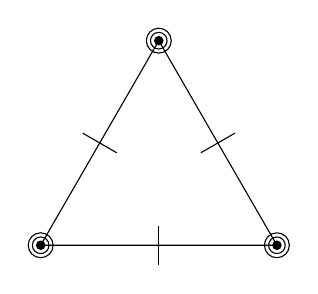
\begin{tikzpicture}[scale=0.5]
	%define the vertices of the triangle
	\path[coordinate] (0,0) coordinate(A)
		++(60:3cm) coordinate(D)
		++(60:3cm) coordinate(B)
		++(-60:3cm) coordinate(E)
		++(-60:3cm) coordinate(C)
		++(180:3cm) coordinate(F);
	%label the vertices and draw edges
	\draw (A) -- (D) -- (B) -- (E) -- (C) -- (F) -- cycle;
	%draw the interpolation points
	%function values
	\filldraw[black] (A) circle(3pt); 
	\filldraw[black] (B) circle(3pt); 
	\filldraw[black] (C) circle(3pt); 
	%first derivatives
	\draw[black] (A) circle(6pt); 
	\draw[black] (B) circle(6pt); 
	\draw[black] (C) circle(6pt); 
	%second derivatives
	\draw[black] (A) circle(9pt); 
	\draw[black] (B) circle(9pt); 
	\draw[black] (C) circle(9pt); 
	%normal derivatives
	\draw (1.067,2.848) -- (D) -- (1.933,2.348); 
	\draw (4.067,2.348) -- (E) -- (4.933,2.848); 
	\draw (3,-0.5cm) -- (F) -- (3,0.5cm); 
	%labels
%	\node[below of=A, node distance=0.5cm] (k) {$k=j+1$};
% \node[above of=B, node distance=0.5cm] (j) {$j=i+1$};
%	\node[below of=C, node distance=0.5cm] (i) {$i$};
\end{tikzpicture}
	\end{center}
	\caption{Argyris element with its 21 degrees of freedom.}
	\label{fig:Argyris}
\end{figure}

  %If we are to require conforming finite elements, Lagrange finite elements are
not enough to guarantee continuity in the first derivative, and so to ensure
continuity in the first derivative \cite{Johnson} the Argyris Element (depicted
in \autoref{fig:Argyris}) will be required. The Argyris element is probably the
best known of all $C^1$ finite elements \cite{Argyris,Dominguez08}, but appear
to be rarely implemented.

\begin{figure}[h]
	\begin{center}
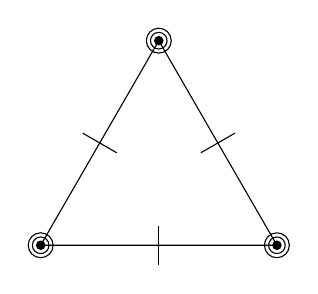
\begin{tikzpicture}[scale=0.5]
	%define the vertices of the triangle
	\path[coordinate] (0,0) coordinate(A)
		++(60:3cm) coordinate(D)
		++(60:3cm) coordinate(B)
		++(-60:3cm) coordinate(E)
		++(-60:3cm) coordinate(C)
		++(180:3cm) coordinate(F);
	%label the vertices and draw edges
	\draw (A) -- (D) -- (B) -- (E) -- (C) -- (F) -- cycle;
	%draw the interpolation points
	%function values
	\filldraw[black] (A) circle(3pt); 
	\filldraw[black] (B) circle(3pt); 
	\filldraw[black] (C) circle(3pt); 
	%first derivatives
	\draw[black] (A) circle(6pt); 
	\draw[black] (B) circle(6pt); 
	\draw[black] (C) circle(6pt); 
	%second derivatives
	\draw[black] (A) circle(9pt); 
	\draw[black] (B) circle(9pt); 
	\draw[black] (C) circle(9pt); 
	%normal derivatives
	\draw (1.067,2.848) -- (D) -- (1.933,2.348); 
	\draw (4.067,2.348) -- (E) -- (4.933,2.848); 
	\draw (3,-0.5cm) -- (F) -- (3,0.5cm); 
	%labels
%	\node[below of=A, node distance=0.5cm] (k) {$k=j+1$};
% \node[above of=B, node distance=0.5cm] (j) {$j=i+1$};
%	\node[below of=C, node distance=0.5cm] (i) {$i$};
\end{tikzpicture}
	\end{center}
	\caption{Argyris element with its 21 degrees of freedom.}
	\label{fig:Argyris}
\end{figure}


The Argyris element does, in fact, ensure $C^1$ continuity
\cite{Dominguez08,Okabe}, but at a cost of twenty-one degrees of freedom.
However, these twenty-one degrees of freedom give basis polynomials of degree
five and therefore has a very high rate of convergence \cite{Dominguez08}.
These degrees of freedom include the value at each vertex, the value of the
first derivatives at each vertex, the value of the second derivatives at each
vertex, the value of the mixed derivative at each vertex, and finally the value
of the normal derivatives at each of the edge midpoints. Here in lies the main
difficulty in implementing the Argyris triangle, the normal derivatives. Not
only do we now have 21 degrees of freedom that we must worry about, but the
added complexity of a transformation that maintains the direction of the normal
derivatives is required. Since working on the reference element is the most
common way of working with finite elements and normal derivatives are not
respected by affine transformation a more complicated transformation will have
to be employed. This is unlike a standard Lagrange element where only a simple
Affine transformation is required. \cite{Dominguez08}

Dominguez \emph{et al.} developed such a transformation. This transformation,
which is a $21 \times 21$ matrix, $C$, allows for all calculations to be done on
a reference element, vastly simplifying the calculations for the various
matrices and load vector required for the QGE finite elements calculations and
allowing for faster running code. Since, the tranformation of Dominguez is so
new and is not the standard for implementation of the Argyris element his
transformation will be discussed at length in \autoref{sse:Trans} for
completeness.


    \section{SQGE Finite Element Discretization} \label{sec:SQGEFEM}
    In this section, we present the functional setting and some auxiliary results
for the FE discretization of the streamfunction formulation of the SQGE
\eqref{eqn:SQGEWF}. Let $\mathcal{T}^h$ denote a finite element triangulation of
$\Omega$ with meshsize (maximum triangle diameter) $h$. We consider a
\emph{conforming} FE discretization of \eqref{eqn:SQGEWF}, i.e., $X^h \subset X
= H_0^2(\Omega)$.

The FE discretization of the streamfunction formulation of the SQGE
\eqref{eqn:SQGEWF} reads:
\begin{equation}
  \begin{split}
    &\text{Find } \psi^h \in X^h \text{ such that} \\
    Re^{-1}(\Delta \psi^h, \Delta \chi^h)
      + b(\psi^h,\psi^h,&\chi^h)
      - Ro^{-1} (\psi_x^h,\chi^h)
      = Ro^{-1}(F,\chi^h),\quad \forall \, \chi^h \in X^h.
    \label{eqn:SQGEFEF}
  \end{split}
\end{equation}
Using standard arguments \cite{Girault79,Girault86}, one can prove that, if the
small data condition used in proving the well-posedness result for the
continuous case holds, then \eqref{eqn:SQGEFEF} has a unique solution $\psi^h$
(see Theorem 2.1 in \cite{Cayco86}). Furthermore, one can prove the following
stability result for $\psi^h$ using the same arguments as those used in the
proof of \eqref{thm:stability_sqge} for the continuous setting.
\begin{thm} \label{thm:stability_fem_sqge} The
  solution $\psi^h$ of \eqref{eqn:SQGEFEF} satisfies the following stability estimate:
 \begin{equation}
   |\psi^h|_2 \le Re \, Ro^{-1} \, \| F \|_{-2} .
   \label{eqn:stability_fem_sqge}
 \end{equation}
\end{thm}
\begin{proof}
  The proof is almost identical to the proof of \autoref{thm:stability_sqge},
  but is given here for completeness.

  Let $\chi^h = \psi^h$ in \eqref{eqn:SQGEFEF} which gives
  \begin{equation*}
    Re^{-1}(\Delta \psi^h, \Delta \psi^h)
      + b(\psi^h,\psi^h,\psi^h)
      - Ro^{-1} (\psi_x^h,\psi^h)
      = Ro^{-1} (F,\psi^h)\qquad  \forall \pi^h \in X^h.
  \end{equation*}
  Since, $b(\psi^h, \psi^h, \psi^h) =0$ and $(\psi_x^h,\psi^h)=0$ we have
  \begin{align*}
    Re^{-1}(\Delta \psi^h, \Delta \psi^h) &= Ro^{-1} (F,\psi^h) \\
    Re^{-1}\, \|\psi^h\|_2^2 &= Ro^{-1}\, (F,\psi^h) \\
    \|\psi^h\|_2 &\le Re\, Ro^{-1}\,\sup_{\psi^h \in X^h} \frac{(F,\psi^h)}{|\psi^h|_2} \\
    \|\psi^h\|_2 &\le Re\, Ro^{-1}\, \|F\|_{-2}.
  \end{align*}
  Thus, the proof is complete.
\end{proof}

Again, we point out that as noted in Section 6.1 in \cite{Ciarlet} (see also
Section 13.2 in \cite{Gunzburger89}, Section 3.1 in \cite{Johnson}, and Theorem
5.2 in \cite{Braess}), in order to develop a conforming FE discretization for the
SQGE \eqref{eqn:SQGEWF}, we are faced with the problem of constructing subspaces
of the space $H^2_0(\Omega)$.  As was discussed previously the Argyris finite
element is an element of class $C^1$ and therefore will be the FE used in this
thesis for the discretization of the SQGE.


    \section{Argyris Element} \label{sec:Argyris}
    If we are to require conforming finite elements, Lagrange finite elements are
not enough to guarantee continuity in the first derivative, and so to ensure
continuity in the first derivative \cite{Johnson} the Argyris Element (depicted
in \autoref{fig:Argyris}) will be required. The Argyris element is probably the
best known of all $C^1$ finite elements \cite{Argyris,Dominguez08}, but appear
to be rarely implemented.

\begin{figure}[h]
	\begin{center}
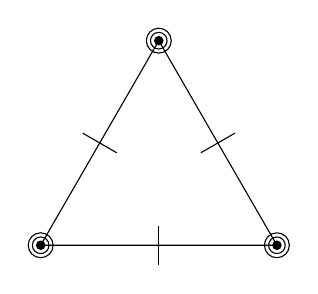
\begin{tikzpicture}[scale=0.5]
	%define the vertices of the triangle
	\path[coordinate] (0,0) coordinate(A)
		++(60:3cm) coordinate(D)
		++(60:3cm) coordinate(B)
		++(-60:3cm) coordinate(E)
		++(-60:3cm) coordinate(C)
		++(180:3cm) coordinate(F);
	%label the vertices and draw edges
	\draw (A) -- (D) -- (B) -- (E) -- (C) -- (F) -- cycle;
	%draw the interpolation points
	%function values
	\filldraw[black] (A) circle(3pt); 
	\filldraw[black] (B) circle(3pt); 
	\filldraw[black] (C) circle(3pt); 
	%first derivatives
	\draw[black] (A) circle(6pt); 
	\draw[black] (B) circle(6pt); 
	\draw[black] (C) circle(6pt); 
	%second derivatives
	\draw[black] (A) circle(9pt); 
	\draw[black] (B) circle(9pt); 
	\draw[black] (C) circle(9pt); 
	%normal derivatives
	\draw (1.067,2.848) -- (D) -- (1.933,2.348); 
	\draw (4.067,2.348) -- (E) -- (4.933,2.848); 
	\draw (3,-0.5cm) -- (F) -- (3,0.5cm); 
	%labels
%	\node[below of=A, node distance=0.5cm] (k) {$k=j+1$};
% \node[above of=B, node distance=0.5cm] (j) {$j=i+1$};
%	\node[below of=C, node distance=0.5cm] (i) {$i$};
\end{tikzpicture}
	\end{center}
	\caption{Argyris element with its 21 degrees of freedom.}
	\label{fig:Argyris}
\end{figure}


The Argyris element does, in fact, ensure $C^1$ continuity
\cite{Dominguez08,Okabe}, but at a cost of twenty-one degrees of freedom.
However, these twenty-one degrees of freedom give basis polynomials of degree
five and therefore has a very high rate of convergence \cite{Dominguez08}.
These degrees of freedom include the value at each vertex, the value of the
first derivatives at each vertex, the value of the second derivatives at each
vertex, the value of the mixed derivative at each vertex, and finally the value
of the normal derivatives at each of the edge midpoints. Here in lies the main
difficulty in implementing the Argyris triangle, the normal derivatives. Not
only do we now have 21 degrees of freedom that we must worry about, but the
added complexity of a transformation that maintains the direction of the normal
derivatives is required. Since working on the reference element is the most
common way of working with finite elements and normal derivatives are not
respected by affine transformation a more complicated transformation will have
to be employed. This is unlike a standard Lagrange element where only a simple
Affine transformation is required. \cite{Dominguez08}

Dominguez \emph{et al.} developed such a transformation. This transformation,
which is a $21 \times 21$ matrix, $C$, allows for all calculations to be done on
a reference element, vastly simplifying the calculations for the various
matrices and load vector required for the QGE finite elements calculations and
allowing for faster running code. Since, the tranformation of Dominguez is so
new and is not the standard for implementation of the Argyris element his
transformation will be discussed at length in \autoref{sse:Trans} for
completeness.

      \subsection{Basis Functions} \label{sse:Basis}
      %In this subsection we derive the basis for the Argyris element using the
%standard Cartesian coordinates on a reference triangle $\hat{K}$ as opposed to
%the area coordinates on a general triangle $K$ as used by \cite{Okabe}.
%The transformation developed by \cite{Dominguez08}, which will be discussed in \autoref{sse:Trans}, allows for all computations to be done on the reference triangle
%and so the bulk of the discussion will be concerned with developing the basis
%functions on $\hat{K}$ and the transformation.
\begin{figure}%[H]
	\begin{center}
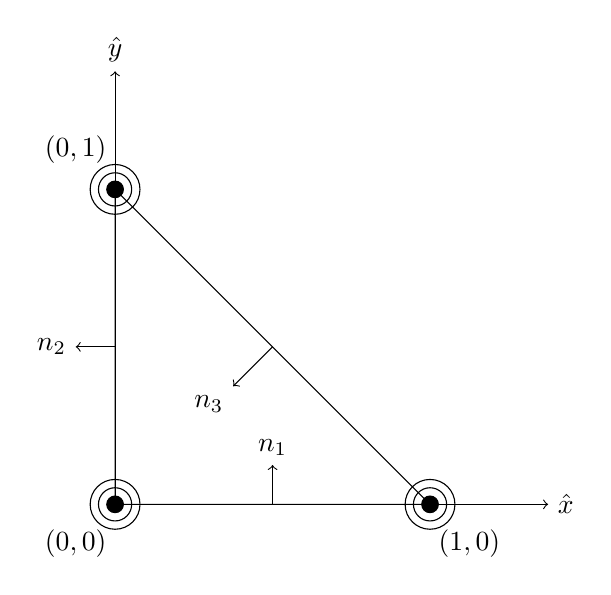
\begin{tikzpicture}
  %draw the axes
  \draw[->] (0,0) -- (5.5,0) node[right,fill=none] {$\hat{x}$};
  \draw[->] (0,0) -- (0,5.5) node[above,fill=none] {$\hat{y}$};
  %draw the triangle
	\draw (0,0) -- (4,0) -- (0,4) -- cycle;
	%draw the interpolation points
	%function values
	\filldraw (0,0) circle(3pt);
	\filldraw (4,0) circle(3pt);
	\filldraw (0,4) circle(3pt);
	%first derivatives
	\draw (0,0) circle(6pt);
	\draw (4,0) circle(6pt);
	\draw (0,4) circle(6pt);
	%second derivatives
	\draw (0,0) circle(9pt);
	\draw (4,0) circle(9pt);
	\draw (0,4) circle(9pt);
	%normal derivatives
  \draw[->] (2,0) -- (2,0.5) node[above,fill=none] {$n_1$};
  \draw[->] (0,2) -- (-0.5,2) node[left,fill=none] {$n_2$};
  \draw[->] (2,2) -- (1.5,1.5) node[below left,fill=none] {$n_3$};
  %label vertices
  %\node[circle] at (-0.6,0) {$1$};
  %\node at (4,-0.6) {$2$};
  %\node at (-0.6,4) {$3$};
  \node at (-0.5,-0.5) {$(0,0)$};
  \node at (4.5,-0.5) {$(1,0)$};
  \node at (-0.5,4.5) {$(0,1)$};
\end{tikzpicture}
	\end{center}
  \caption{The reference triangle $\hat{K}$ for the Argyris element.}
	\label{fig:RefTriangle}
\end{figure}


In most references, which present the Argyris element, only the constraints
found in \autoref{tab:Constraints} are presented. Thus, for completeness, we
derive and explicitly state the the basis functions for the Argyris FE in this
subsection. The Argyris triangle has 21 degrees of freedom and therefore has 21
basis functions per triangle.  Additionally, the basis for Argyris in reference
coordinates (depicted in \autoref{fig:RefTriangle}) belong to the space
$\mathbb{P}_5$, which has the standard monomial basis
\begin{equation*}
	\left\{
    1, x, y, x^2, xy, y^2, x^3, x^2y, xy^2, y^3, x^4, x^3y,
    x^2y^2, xy^3, y^4, x^5, x^4y, x^3y^2, x^2y^3, xy^4, y^5.
  \right\}
\end{equation*}
Thus, the $i^{th}$ basis function for the Argyris triangle can be written as
\begin{equation}
	\begin{split}
	\hat{\varphi}_i(\hat{x},\hat{y}) = m^i_1 + m^i_2 \hat{x} + m^i_3 \hat{x}^2 + m^i_4 \hat{x}^3 + m^i_5 \hat{x}^4 + m^i_6 \hat{x}^5 + m^i_7 \hat{y} + m^i_8
 	\hat{y}^2 + m^i_9 \hat{y}^3 \\
 + m^i_{10} \hat{y}^4 + m^i_{11} \hat{y}^5 + m^i_{12}  \hat{x} \hat{y} + m^i_{13} \hat{x} \hat{y}^2 + m^i_{14} \hat{x} \hat{y}^3 + m^i_{15}
 	\hat{x} \hat{y}^4 + m^i_{16} \hat{x}^2 \hat{y} \\
 + m^i_{17} \hat{x}^2 \hat{y}^2 + m^i_{18}\hat{x}^2 \hat{y}^3 + m^i_{19} \hat{x}^3 \hat{y} + m^i_{20}\hat{x}^3 \hat{y}^2 + m^i_{21} \hat{x}^4 \hat{y}.
 \end{split}
	\label{eqn:Basis}
\end{equation}

Now, consider the reference triangle $\hat{K}$ in Figure \ref{fig:RefTriangle} with
vertices numbered counterclockwise $1,\, 2,\text{ and } 3$, i.e.
$(\hat{x}_1,\hat{y}_1)=(0,0),\, (\hat{x}_2,\hat{y}_2)=(1,0),\text{ and } (\hat{x}_3,\hat{y}_3)=(0,1)$.
Additionally, let the vector $v_i$ represent the $i^{th}$ edge with
\begin{equation*}
  v_1 = [\hat{x}_2-\hat{x}_1,\hat{y}_2-\hat{y}_1]^T, \quad v_2=[\hat{x}_3-\hat{x}_1,\hat{y}_3-\hat{y}_1]^T \text{ and } v_3=[\hat{x}_3
  -\hat{x}_2,\hat{y}_3-\hat{y}_2]^T.
\end{equation*}
For book keeping purposes, we will use the convention that the $i^{th}$ normal
vector is the rotation of the $v_i$ counter-clockwise $90^\circ$. This is the
same convention used by Dominguez et. al. \cite{Dominguez08}. Therefore, the
$i^{th}$ basis function can be found using the restriction in Table
\ref{tab:Constraints}.

\begin{table}%[H]
\begin{center}
  {\tiny\begin{tabular}{|p{1.2in}|p{1.2in}|p{1.2in}|}
	\hline
	$i,j,k=1,2,3$ & $i=4,5,6$ and $j,k=1,2,3$ &
	$i=7,8,9$ and $j,k=1,2,3$ \\
	\hline
	\begin{equation*}
		\begin{split}
		\varphi_i (x_j,y_j) = \delta_{i,j} \\
		\dfrac{\partial \varphi_i}{\partial x} (x_j,y_j) = 0 \\
		\dfrac{\partial \varphi_i}{\partial y} (x_j,y_j) = 0 \\
		\dfrac{\partial^2 \varphi_i}{\partial x^2} (x_j,y_j) = 0 \\
		\dfrac{\partial^2 \varphi_i}{\partial x \partial y} (x_j,y_j) = 0 \\
		\dfrac{\partial^2 \varphi_i}{\partial y^2} (x_j,y_j) = 0 \\
		\dfrac{\partial\varphi_i}{\partial n_k} = 0
		\end{split}
	\end{equation*} &
	\begin{equation*}
		\begin{split}
		\varphi_i (x_j,y_j) = 0 \\
		\dfrac{\partial \varphi_i}{\partial x} (x_j,y_j) = \delta_{i,j+3} \\
		\dfrac{\partial \varphi_i}{\partial y} (x_j,y_j) = 0 \\
		\dfrac{\partial^2 \varphi_i}{\partial x^2} (x_j,y_j) = 0 \\
		\dfrac{\partial^2 \varphi_i}{\partial x \partial y} (x_j,y_j) = 0 \\
		\dfrac{\partial^2 \varphi_i}{\partial y^2} (x_j,y_j) = 0 \\
		\dfrac{\partial\varphi_i}{\partial n_k} = 0
		\end{split}
	\end{equation*} &
	\begin{equation*}
		\begin{split}
		\varphi_i (x_j,y_j) = 0 \\
		\dfrac{\partial \varphi_i}{\partial x} (x_j,y_j) = 0 \\
		\dfrac{\partial \varphi_i}{\partial y} (x_j,y_j) = \delta_{i,j+6} \\
		\dfrac{\partial^2 \varphi_i}{\partial x^2} (x_j,y_j) = 0 \\
		\dfrac{\partial^2 \varphi_i}{\partial x \partial y} (x_j,y_j) = 0 \\
		\dfrac{\partial^2 \varphi_i}{\partial y^2} (x_j,y_j) = 0 \\
		\dfrac{\partial\varphi_i}{\partial n_k} = 0
		\end{split}
	\end{equation*} \\
	\hline
	\hline
	$i=10,11,12$ and $j,k=1,2,3$
	& $i=13,14,15$ and $j,k=1,2,3$ &
	$i=16,17,18$ and $j,k=1,2,3$ \\
	\hline
	\begin{equation*}
		\begin{split}
		\varphi_i (x_j,y_j) = 0 \\
		\dfrac{\partial \varphi_i}{\partial x} (x_j,y_j) = 0 \\
		\dfrac{\partial \varphi_i}{\partial y} (x_j,y_j) = 0 \\
		\dfrac{\partial^2 \varphi_i}{\partial x^2} (x_j,y_j) = \delta_{i,j+9} \\
		\dfrac{\partial^2 \varphi_i}{\partial x \partial y} (x_j,y_j) = 0 \\
		\dfrac{\partial^2 \varphi_i}{\partial y^2} (x_j,y_j) = 0 \\
		\dfrac{\partial\varphi_i}{\partial n_k} = 0
		\end{split}
	\end{equation*} &
	\begin{equation*}
		\begin{split}
		\varphi_i (x_j,y_j) = 0 \\
		\dfrac{\partial \varphi_i}{\partial x} (x_j,y_j) = 0 \\
		\dfrac{\partial \varphi_i}{\partial y} (x_j,y_j) = 0 \\
		\dfrac{\partial^2 \varphi_i}{\partial x^2} (x_j,y_j) = 0 \\
		\dfrac{\partial^2 \varphi_i}{\partial x \partial y} (x_j,y_j) = 0 \\
		\dfrac{\partial^2 \varphi_i}{\partial y^2} (x_j,y_j) = \delta_{i,j+12} \\
		\dfrac{\partial\varphi_i}{\partial n_k} = 0
		\end{split}
	\end{equation*} &
	\begin{equation*}
		\begin{split}
		\varphi_i (x_j,y_j) = 0 \\
		\dfrac{\partial \varphi_i}{\partial x} (x_j,y_j) = 0 \\
		\dfrac{\partial \varphi_i}{\partial y} (x_j,y_j) = 0 \\
		\dfrac{\partial^2 \varphi_i}{\partial x^2} (x_j,y_j) = 0 \\
		\dfrac{\partial^2 \varphi_i}{\partial x \partial y} (x_j,y_j) = \delta_{i,j+15} \\
		\dfrac{\partial^2 \varphi_i}{\partial y^2} (x_j,y_j) = 0 \\
		\dfrac{\partial\varphi_i}{\partial n_k} = 0
		\end{split}
	\end{equation*} \\
	\hline
	\hline
	& $i=19,20,21$ and $k=1,2,3$ & \\
	\hline
	& \begin{equation*}
		\begin{split}
		\varphi_i (x_j,y_j) = 0 \\
		\dfrac{\partial \varphi_i}{\partial x} (x_j,y_j) = 0 \\
		\dfrac{\partial \varphi_i}{\partial y} (x_j,y_j) = 0 \\
		\dfrac{\partial^2 \varphi_i}{\partial x^2} (x_j,y_j) = 0 \\
		\dfrac{\partial^2 \varphi_i}{\partial x \partial y} (x_j,y_j) = 0 \\
		\dfrac{\partial^2 \varphi_i}{\partial y^2} (x_j,y_j) = 0 \\
		\dfrac{\partial\varphi_i}{\partial n_k} = \delta_{i,k-18}
		\end{split}
	\end{equation*} & \\
	\hline
\end{tabular}}
\caption{Constraints for Argyris triangle
  \cite{Argyris,Brenner,Ciarlet,Dominguez08}}
\label{tab:Constraints}
\end{center}
\end{table}


Now, let $z$ be the vector containing the monomial basis for $\mathbb{P}_5$, i.e.
\small{
\begin{equation*}
  z=\left[
    1, \hat{x}, \hat{y}, \hat{x}^2, \hat{x}\hat{y}, \hat{y}^2, \hat{x}^3, \hat{x}^2\hat{y}, \hat{x}\hat{y}^2, \hat{y}^3, \hat{x}^4, \hat{x}^3\hat{y},
    \hat{x}^2\hat{y}^2, \hat{x}\hat{y}^3, \hat{y}^4, \hat{x}^5, \hat{x}^4\hat{y}, \hat{x}^3\hat{y}^2, \hat{x}^2\hat{y}^3, \hat{x}\hat{y}^4, \hat{y}^4
  \right]^{T}
\end{equation*}}
Then the $i^{th}$ Argyris basis function on $\hat{K}$ is given by
\begin{equation*}
  \hat{\varphi}_i = M_i z,
\end{equation*}
where $M_i$ is the $i^{th}$ row of the matrix $M$. Therefore, the evaluation of
$\hat{\varphi}_i(\hat{x},\hat{y})$ comes down to the matrix-vector multiplication
\begin{equation*}
  \hat{\varphi}_i(\hat{x},\hat{y}) = M_i z(\hat{x},\hat{y}).
\end{equation*}

To determine the matrix $M$ we must solve the linear system
\begin{equation*}
  ZM^T=I_{21}
\end{equation*}
that results from the constraints in Table \ref{tab:Constraints}. Here
\begin{equation*}
  \begin{split}Z=[z(0,0), z(0,1), z(1,0),
  z_{\hat{x}}(0,0), z_{\hat{y}}(0,0),
  z_{\hat{x}}(1,0), z_{\hat{y}}(1,0),
  z_{\hat{x}}(0,1), z_{\hat{y}}(0,1), \\
  z_{\hat{x}\hat{x}}(0,0), z_{\hat{x}\hat{y}}(0,0), z_{\hat{y}\hat{y}}(0,0),
  z_{\hat{x}\hat{x}}(1,0), z_{\hat{x}\hat{y}}(1,0), z_{\hat{y}\hat{y}}(1,0), \\
  z_{\hat{x}\hat{x}}(0,1), z_{\hat{x}\hat{y}}(0,1), z_{\hat{y}\hat{y}}(0,1),
  z_{\hat{y}}(\nicefrac{1}{2},0), -z_{\hat{x}}(0,\nicefrac{1}{2}), \\
  -\frac{1}{\sqrt{2}}(z_{\hat{x}}(\nicefrac{1}{2},\nicefrac{1}{2}) +
  z_{\hat{y}}(\nicefrac{1}{2},\nicefrac{1}{2}))]^T.\end{split}
\end{equation*}
$I_{21}$ is a $21\times 21$ identity matrix and $M$ is the matrix containing the
coefficients for all 21 basis functions. Therefore solving this system will
result in a matrix, $M$, that contains the coefficients for the Argyris basis
functions for the reference triangle as in \eqref{eqn:Basis}. Thus, the matrix
$M$ is \\
%\begin{sideways}
%\begin{minipage}[h]{0.7\textheight}
%  \vspace{0.25\textwidth}
\begin{sidewaystable}%[H]
  \begin{center}
{\small%tiny
\begin{equation*}
 \left[\begin{array}{ccccccccccccccccccccc}
1 & 0 & 0 & 0 & 0 & 0 & -10 & 0 & 0 & -10 & 15 & 0 & -30 & 0 & 15 & -6 & 0 & 30 & 30 & 0 & -6 \\[0.5em]
0 & 0 & 0 & 0 & 0 & 0 & 10 & 0 & 0 & 0 & -15 & 0 & 15 & 0 & 0 & 6 & 0 & -15 & -15 & 0 & 0 \\[0.5em]
0 & 0 & 0 & 0 & 0 & 0 & 0 & 0 & 0 & 10 & 0 & 0 & 15 & 0 & -15 & 0 & 0 & -15 & -15 & 0 & 6 \\[0.5em]
0 & 1 & 0 & 0 & 0 & 0 & -6 & 0 & -11 & 0 & 8 & 0 & 10 & 18 & 0 & -3 & 0 & 1 & -10 & -8 & 0 \\[0.5em]
0 & 0 & 1 & 0 & 0 & 0 & 0 & -11 & 0 & -6 & 0 & 18 & 10 & 0 & 8 & 0 & -8 & -10 & 1 & 0 & -3 \\[0.5em]
0 & 0 & 0 & 0 & 0 & 0 & -4 & 0 & 0 & 0 & 7 & 0 & -\frac{7}{2} & 0 & 0 & -3 & 0 & \frac{7}{2} & \frac{7}{2} & 0 & 0 \\[0.5em]
0 & 0 & 0 & 0 & 0 & 0 & 0 & -5 & 0 & 0 & 0 & 14 & \frac{37}{2} & 0 & 0 & 0 & -8 & -\frac{37}{2} & -\frac{27}{2} & 0 & 0 \\[0.5em]
0 & 0 & 0 & 0 & 0 & 0 & 0 & 0 & -5 & 0 & 0 & 0 & \frac{37}{2} & 14 & 0 & 0 & 0 & -\frac{27}{2} & -\frac{37}{2} & -8 & 0 \\[0.5em]
0 & 0 & 0 & 0 & 0 & 0 & 0 & 0 & 0 & -4 & 0 & 0 & -\frac{7}{2} & 0 & 7 & 0 & 0 & \frac{7}{2} & \frac{7}{2} & 0 & -3 \\[0.5em]
0 & 0 & 0 & \frac{1}{2} & 0 & 0 & -\frac{3}{2} & 0 & 0 & 0 & \frac{3}{2} & 0 & -\frac{3}{2} & 0 & 0 & -\frac{1}{2} & 0 & \frac{3}{2} & 1 & 0 & 0 \\[0.5em]
0 & 0 & 0 & 0 & 1 & 0 & 0 & -4 & -4 & 0 & 0 & 5 & 10 & 5 & 0 & 0 & -2 & -6 & -6 & -2 & 0 \\[0.5em]
0 & 0 & 0 & 0 & 0 & \frac{1}{2} & 0 & 0 & 0 & -\frac{3}{2} & 0 & 0 & -\frac{3}{2} & 0 & \frac{3}{2} & 0 & 0 & 1 & \frac{3}{2} & 0 & -\frac{1}{2} \\[0.5em]
0 & 0 & 0 & 0 & 0 & 0 & \frac{1}{2} & 0 & 0 & 0 & -1 & 0 & \frac{1}{4} & 0 & 0 & \frac{1}{2} & 0 & -\frac{1}{4} & -\frac{1}{4} & 0 & 0 \\[0.5em]
0 & 0 & 0 & 0 & 0 & 0 & 0 & 1 & 0 & 0 & 0 & -3 & -\frac{7}{2} & 0 & 0 & 0 & 2 & \frac{7}{2} & \frac{5}{2} & 0 & 0 \\[0.5em]
0 & 0 & 0 & 0 & 0 & 0 & 0 & 0 & 0 & 0 & 0 & 0 & \frac{5}{4} & 0 & 0 & 0 & 0 & -\frac{3}{4} & -\frac{5}{4} & 0 & 0 \\[0.5em]
0 & 0 & 0 & 0 & 0 & 0 & 0 & 0 & 0 & 0 & 0 & 0 & \frac{5}{4} & 0 & 0 & 0 & 0 & -\frac{5}{4} & -\frac{3}{4} & 0 & 0 \\[0.5em]
0 & 0 & 0 & 0 & 0 & 0 & 0 & 0 & 1 & 0 & 0 & 0 & -\frac{7}{2} & -3 & 0 & 0 & 0 & \frac{5}{2} & \frac{7}{2} & 2 & 0 \\[0.5em]
0 & 0 & 0 & 0 & 0 & 0 & 0 & 0 & 0 & \frac{1}{2} & 0 & 0 & \frac{1}{4} & 0 & -1 & 0 & 0 & -\frac{1}{4} & -\frac{1}{4} & 0 & \frac{1}{2} \\[0.5em]
0 & 0 & 0 & 0 & 0 & 0 & 0 & 16 & 0 & 0 & 0 & -32 & -32 & 0 & 0 & 0 & 16 & 32 & 16 & 0 & 0 \\[0.5em]
0 & 0 & 0 & 0 & 0 & 0 & 0 & 0 & -16 & 0 & 0 & 0 & 32 & 32 & 0 & 0 & 0 & -16 & -32 & -16 & 0 \\[0.5em]
0 & 0 & 0 & 0 & 0 & 0 & 0 & 0 & 0 & 0 & 0 & 0 & 8\sqrt{2} & 0 & 0 & 0 & 0 & -8\sqrt{2} & -8\sqrt{2} & 0 & 0
  \end{array}\right]
\end{equation*}
}
\caption{Coefficients for the Argyris basis matrix, $M$.}
\label{tab:Coefficients}
  \end{center}
\end{sidewaystable}
%\end{minipage}
%\end{sideways} \\


Therefore, the Argyris basis functions, on the reference element $\hat{K}$, are
\begin{equation}
\begin{split}
  \hat{\varphi}_1(\hat{x},\hat{y}) &= 1-10\hat{x}^3-10\hat{y}^3+15\hat{x}^4-30\hat{x}^2\hat{y}^2+15\hat{y}^4-6\hat{x}^5+30\hat{x}^3\hat{y}^2+30\hat{x}^2\hat{y}^3-6\hat{y}^5 \\
  \hat{\varphi}_2(\hat{x},\hat{y}) &= 10\hat{x}^3-15\hat{x}^4+15\hat{x}^2\hat{y}^2+6\hat{x}^5-15\hat{x}^3\hat{y}^2-15\hat{x}^2\hat{y}^3 \\
  \hat{\varphi}_3(\hat{x},\hat{y}) &= 10\hat{y}^3+15\hat{x}^2\hat{y}^2-15\hat{y}^4-15\hat{x}^3\hat{y}^2-15\hat{x}^2\hat{y}^3+6\hat{y}^2 \\
  \hat{\varphi}_4(\hat{x},\hat{y}) &= \hat{x}-6\hat{x}^3-11\hat{x}\hat{y}^2+8\hat{x}^4+10\hat{x}^2\hat{y}^2+18\hat{x}\hat{y}^3-3\hat{x}^5+\hat{x}^3\hat{y}^2-10\hat{x}^2\hat{y}^3-8\hat{x}\hat{y}^4 \\
  \hat{\varphi}_5(\hat{x},\hat{y}) &= \hat{y}-11\hat{x}^2\hat{y}-6\hat{y}^3+18\hat{x}^3\hat{y}+10\hat{x}^2\hat{y}^2+8\hat{y}^4-8\hat{x}^4\hat{y}-10\hat{x}^3\hat{y}^2+\hat{x}^2\hat{y}^3-3\hat{y}^5 \\
  \hat{\varphi}_6(\hat{x},\hat{y}) &= -4\hat{x}^3+7\hat{x}^4-\frac{7}{2}\hat{x}^2\hat{y}^2-3\hat{x}^5+\frac{7}{2}\hat{x}^3\hat{y}^2+\frac{7}{2}\hat{x}^2\hat{y}^3 \\
  \hat{\varphi}_7(\hat{x},\hat{y}) &= -5\hat{x}^2\hat{y}+14\hat{x}^3\hat{y}+\frac{37}{2}\hat{x}^2\hat{y}^2-8\hat{x}^4\hat{y}-\frac{37}{2}\hat{x}^3\hat{y}^2-\frac{27}{2}\hat{x}^2\hat{y}^3 \\
  \hat{\varphi}_8(\hat{x},\hat{y}) &= -5\hat{x}\hat{y}^2+\frac{37}{2}\hat{x}^2\hat{y}^2+14\hat{x}\hat{y}^3-\frac{27}{2}\hat{x}^3\hat{y}^2-\frac{37}{2}\hat{x}^3\hat{y}^2-8\hat{x}\hat{y}^4 \\
  \hat{\varphi}_9(\hat{x},\hat{y}) &= -4\hat{y}^3-\frac{7}{2}\hat{x}^3+7\hat{y}^4+\frac{7}{2}\hat{x}^3\hat{y}^2+\frac{7}{2}\hat{x}^2\hat{y}^3-3\hat{y}^5 \\
  \hat{\varphi}_{10}(\hat{x},\hat{y}) &= \frac{1}{2}\hat{x}^2-\frac{3}{2}\hat{x}^3+\frac{3}{2}\hat{x}^4-\frac{3}{2}\hat{x}^2\hat{y}^2-\frac{1}{2}\hat{x}^5+\frac{3}{2}\hat{x}^3\hat{y}^2+\hat{x}^2\hat{y}^3 \\
  \hat{\varphi}_{11}(\hat{x},\hat{y}) &= \hat{x}\hat{y}-4\hat{x}^2\hat{y}-4\hat{x}\hat{y}^2+5\hat{x}^3\hat{y}+10\hat{x}^2\hat{y}^2+5\hat{x}\hat{y}^3-2\hat{x}^4\hat{y}-6\hat{x}^3\hat{y}^2-6\hat{x}^2\hat{y}^3-2\hat{x}\hat{y}^4 \\
  \hat{\varphi}_{12}(\hat{x},\hat{y}) &= \frac{1}{2}\hat{y}^2-\frac{3}{2}\hat{y}^3-\frac{3}{2}\hat{x}^2\hat{y}^2+\frac{3}{2}\hat{y}^4+\hat{x}^3\hat{y}^2+\frac{3}{2}\hat{x}^2\hat{y}^3-\frac{1}{2}\hat{y}^5 \\
  \hat{\varphi}_{13}(\hat{x},\hat{y}) &= \frac{1}{2}\hat{x}^3-\hat{x}^4+\frac{1}{4}\hat{x}^2\hat{y}^2+\frac{1}{2}\hat{x}^5-\frac{1}{4}\hat{x}^3\hat{y}^2-\frac{1}{4}\hat{x}^2\hat{y}^3 \\
  \hat{\varphi}_{14}(\hat{x},\hat{y}) &= \hat{x}^2\hat{y}-3\hat{x}^3\hat{y}-\frac{7}{2}\hat{x}^2\hat{y}^2+2\hat{x}^4\hat{y}+\frac{7}{2}\hat{x}^3\hat{y}^2+\frac{5}{2}\hat{x}^2\hat{y}^3 \\
  \hat{\varphi}_{15}(\hat{x},\hat{y}) &= \frac{5}{4}\hat{x}^2\hat{y}^2-\frac{3}{4}\hat{x}^3\hat{y}^2-\frac{5}{4}\hat{x}^2\hat{y}^3 \\
  \hat{\varphi}_{16}(\hat{x},\hat{y}) &= \frac{5}{4}\hat{x}^2\hat{y}^2-\frac{5}{4}\hat{x}^3\hat{y}^2-\frac{3}{4}\hat{x}^2\hat{y}^3 \\
  \hat{\varphi}_{17}(\hat{x},\hat{y}) &= \hat{x}\hat{y}^2-\frac{7}{2}\hat{x}^2\hat{y}^2-3\hat{x}\hat{y}^3+\frac{5}{2}\hat{x}^3\hat{y}^2+\frac{7}{2}\hat{x}^2\hat{y}^3+2\hat{x}\hat{y}^4 \\
  \hat{\varphi}_{18}(\hat{x},\hat{y}) &= \frac{1}{2}\hat{y}^3+\frac{1}{4}\hat{x}^2\hat{y}^2-\hat{y}^4-\frac{1}{4}\hat{x}^3\hat{y}^2-\frac{1}{4}\hat{x}^2\hat{y}^3+\frac{1}{2}\hat{y}^5 \\
  \hat{\varphi}_{19}(\hat{x},\hat{y}) &= 16\hat{x}^2\hat{y}-32\hat{x}^3\hat{y}-32\hat{x}^2\hat{y}^2+16\hat{x}^4\hat{y}+32\hat{x}^3\hat{y}^2+16\hat{x}^2\hat{y}^3 \\
  \hat{\varphi}_{20}(\hat{x},\hat{y}) &= -16\hat{x}\hat{y}^2+32\hat{x}^2\hat{y}^2+32\hat{x}\hat{y}^3-16\hat{x}^3\hat{y}^2-32\hat{x}^2\hat{y}^3-16\hat{x}\hat{y}^4 \\
  \hat{\varphi}_{21}(\hat{x},\hat{y}) &= \sqrt{2}\left(8\hat{x}^2\hat{y}^2-8\hat{x}^3\hat{y}^2-8\hat{x}^2\hat{y}^3\right)
\end{split}
\label{eqn:Argyris}
\end{equation}


\begin{remark}
  Throughout our search for an explicit statement of the Argyris basis functions
  we only came across two reference, \cite{Wiki} and \cite{FEM++}, both of which are
  online references. However, this is not to mean that a reference containining
  the explicit statement of the Argyris basis functions doesn't exist, but it
  certainly eluded the author of this thesis.
\end{remark}


      \subsection{Transformation} \label{sse:Trans}
      Now that we have the Argyris basis functions on the reference triangle we need
to relate those to the Argyris basis functions on a general triangle. So let's
first consider the affine transformation from $\hat{K}$ to $K$, i.e. $F: \hat{K}
\to K$ such that
\begin{equation}
  F(\hat{\mathbf{x}}) = B\hat{\mathbf{x}} + \mathbf{b} := 
  \begin{bmatrix}
    x_2 - x_1 & x_3 - x_1 \\ y_2 - y_1 & y_3 - y_1
  \end{bmatrix} \begin{bmatrix}
    \hat{x} \\ \hat{y}
  \end{bmatrix} + \begin{bmatrix}
    x_1 \\ y_1
  \end{bmatrix}.
  \label{eqn:Affine}
\end{equation}
Also number the vectors representing the edge of the triangle as
\begin{equation*}
  \mathbf{v}_1 = \mathbf{x}_2 - \mathbf{x}_1\quad \mathbf{v}_2 = \mathbf{x}_3 -
  \mathbf{x}_1\quad \mathbf{v}_3 = \mathbf{x}_3 - \mathbf{x}_2
\end{equation*}
Let $\mathbf{n}_i$ be the unit normal vector corresponding to the $i^{th}$ side obtained by
rotating the vector $\mathbf{v}_i$ by $\nicefrac{\pi}{2}$ in the positive
direction. Additionally, let $\mathbf{m}_i$ be the midpoint to the $i^{th}$
side.
Now consider the linear functionals corresponding to the vertices of the
triangle $K$ numbered as
\begin{align*}
  \mathcal{L}_i(\varphi) &:= \varphi(\mathbf{x}_i), \\
  \mathcal{L}_i^\circ(\varphi) &:= \partial_\circ \varphi(\mathbf{x}_i) \quad \circ \in
    \{x,y\}, \\
  \mathcal{L}_i^\circ(\varphi) &:= \partial_\circ \varphi(\mathbf{x}_i) \quad \circ \in
    \{xx,xy,yy\}
\end{align*}
for $i\in \{1,2,3\}$. For the functionals corresponding to the sides
\begin{equation*}
  \mathcal{L}_i^n(\varphi) := \nabla_{\mathbf{x}} \phi(\mathbf{m}_i) \cdot
  \mathbf{n}_i \quad i\in\{1,2,3\}.
\end{equation*}
Now let's renumber the linear functionals as $\mathcal{L}_j$ for
$j\in\{1,\dots,21\}$ as they are listed below
\begin{align*}
  &\mathcal{L}_1, \mathcal{L}_2, \mathcal{L}_3, \\
  &\mathcal{L}_1^x, \mathcal{L}_1^y, \mathcal{L}_2^x, \mathcal{L}_2^y,
    \mathcal{L}_3^x, \mathcal{L}_3^y, \\ 
  &\mathcal{L}_1^{xx}, \mathcal{L}_1^{xy}, \mathcal{L}_1^{yy},
    \mathcal{L}_2^{xx}, \mathcal{L}_2^{xy}, \mathcal{L}_2^{yy},
    \mathcal{L}_3^{xx}, \mathcal{L}_3^{xy}, \mathcal{L}_3^{yy}, \\
  &\mathcal{L}_1^n, \mathcal{L}_2^n, \mathcal{L}_3^n,
\end{align*}
and the linear functionals $\hat{\mathcal{L}}_i$ and $\hat{ \mathcal{L}_i^n}$
are the corresponding functionals on the reference triangle $\hat{K}$. The basis
functions of the Argyris triangle are fifth degree polynomials in
$\mathbb{P}_5(K)$
that satisfy
\begin{equation*}
  \mathcal{L}_i(\varphi_j) = \delta_{ij} \quad i,j\in\{1,\dots,21\}
\end{equation*}
and similarly on the reference triangle
\begin{equation*}
  \hat{\mathcal{L}}_i(\hat{\varphi}_j) = \delta_{ij} \quad
  i,j\in\{1,\dots,21\}.
\end{equation*}
Now define a new set of functionals such that 
\begin{equation}
  \tilde{\mathcal{L}}_i(\varphi) := \hat{\mathcal{L}}_i(\varphi\circ F).
  \label{eqn:Functional}
\end{equation}
Since $\{\tilde{\mathcal{L}}_i\}$ and $\{\hat{\mathcal{L}}_i\}$ are both basis
for the dual space of $\mathbb{P}_5(K)$ there is a nonsingular matrix $C$ such
that 
\begin{equation}
  \tilde{\mathcal{L}}_i = \sum_{j=1}^{21} c_{ij} \mathcal{L}_j \quad i\in
  \{1,\dots,21\}. 
  \label{eqn:FunctionalsC}
\end{equation}
and therefore it follows
\begin{equation}
  \varphi_i\circ F = \sum_{j=1}^{21} c_{ij}\hat{\varphi}_j \quad i\in
  \{1,\dots,21\}. 
  \label{eqn:PolyC}
\end{equation} \cite{Dominguez08}
Now, we must determine a simple expression for this $C$.

Let's introduce a new set of linear functionals
\begin{equation*}
  \mathcal{L}^*_i \quad i\in\{1,\dots,24\}
\end{equation*}
in the following way; first we let $\mathcal{L}^*_i:=\mathcal{L}_i\;
i=\{1,\dots,18\}$ and then introduce the new functionals
\begin{equation*}
  \mathcal{L}^\circ_i \quad \circ \in \{\perp,||\}\quad i\in \{1,2,3\}
\end{equation*}
by the following relationship
\begin{equation*}
  \mathcal{L}_i^{\perp}(\varphi) := \nabla_{\mathbf{x}} \varphi(\mathbf{m}_i)
  \cdot R\mathbf{v}_i, \quad 
  \mathcal{L}^{||}_i (\varphi) := \nabla_{\mathbf{x}} \varphi(\mathbf{m}_i)
  \cdot \mathbf{v}_i
\end{equation*}
where 
\begin{equation*}
  R = \begin{bmatrix}
    0 & -1 \\ 1 & 0
  \end{bmatrix}
\end{equation*} 
is the matrix that rotates a vector $\nicefrac{\pi}{2}$ counter-clockwise. Now
order the linear functionals as
$\mathcal{L}^{\perp}_1,\mathcal{L}^{\perp}_2,\mathcal{L}^{\perp}_3,
\mathcal{L}^{||}_1,\mathcal{L}^{||}_2,\mathcal{L}^{||}_3$.
Therefore, we have the relationship 
\begin{equation}
  \tilde{\mathcal{L}}_i = \sum_{j=1}^{24} d_{ij} \mathcal{L}^*_j, \quad
    i\in\{1,\dots,21\}.
  \label{eqn:FunctionalsD}
\end{equation}

Now from \eqref{eqn:Affine} we see that 
\begin{align*}
  &\frac{\partial x}{\partial \hat{x}} = B_{11}   &\frac{\partial x}{\partial \hat{y}} = B_{12} \\
  &\frac{\partial y}{\partial \hat{x}} = B_{21}   &\frac{\partial y}{\partial \hat{y}} = B_{22}
\end{align*}
With this we can determine the relationship between the gradient of $\hat{\varphi}$ on the
triangle $\hat{K}$ to the gradient of $\varphi$ on the triangle $K$
\begin{align*}
  \nabla_{\mathbf{\hat{x}}}\left( \varphi \circ F \right) &= \begin{bmatrix}
    \dfrac{\partial \varphi\circ F}{\partial \hat{x}} \\[1em]
    \dfrac{\partial \varphi\circ F}{\partial \hat{y}}
  \end{bmatrix} \\
  &=\begin{bmatrix} 
    \dfrac{\partial \varphi\circ F}{\partial x} \cdot \dfrac{\partial x}{\partial \hat{x}} +
      \dfrac{\partial \varphi\circ F}{\partial y} \cdot \dfrac{\partial y}{\partial \hat{x}} \\[1em]
    \dfrac{\partial \varphi\circ F}{\partial x} \cdot \dfrac{\partial x}{\partial \hat{y}} +
      \dfrac{\partial \varphi\circ F}{\partial y} \cdot \dfrac{\partial y}{\partial \hat{y}} 
  \end{bmatrix} \\
  &= \begin{bmatrix}
    \dfrac{\partial x}{\partial \hat{x}} & \dfrac{\partial y}{\partial \hat{x}} \\[1em]
    \dfrac{\partial x}{\partial \hat{y}} & \dfrac{\partial y}{\partial \hat{y}} 
  \end{bmatrix}\cdot \begin{bmatrix}
    \dfrac{\partial \varphi\circ F}{\partial x} \\[1em] \dfrac{\partial \varphi\circ F}{\partial y} 
  \end{bmatrix}
\end{align*}
and so
\begin{equation}
  \nabla_{\mathbf{\hat{x}}}\left( \varphi \circ F \right) = B^T \nabla_{\mathbf{x}} \varphi \circ F
  \label{eqn:Gradient}
\end{equation}

If we defined the Hessian as $H_x(\varphi) = \left[ \varphi_{xx},\,
\varphi_{xy},\, \varphi_{yy}\right]^T$ then using \eqref{eqn:Affine} we can
determine the relationship between the hessian of $\hat{\varphi}$ on the
triangle $\hat{K}$ to the hessian of $\varphi$ on the triangle $K$
\begin{align*}
  H_{\mathbf{\hat{x}}}(\varphi\circ F) &= \begin{bmatrix} 
    \dfrac{\partial^2 \varphi\circ F}{\partial \hat{x}^2} \\[1em]
    \dfrac{\partial^2 \varphi\circ F}{\partial \hat{x} \partial\hat{y}} \\[1em]
    \dfrac{\partial^2 \varphi\circ F}{\partial \hat{y}^2} 
  \end{bmatrix} \\
  &= \begin{bmatrix} 
    \dfrac{\partial}{\partial \hat{x}}\left( \dfrac{\partial \varphi\circ
      F}{\partial x}\cdot \dfrac{\partial x}{\partial \hat{x}} + \dfrac{\partial
      \varphi\circ F}{\partial y}\cdot \dfrac{\partial y}{\partial
      \hat{x}} \right) \\[1em] 
    \dfrac{\partial}{\partial \hat{y}}\left( \dfrac{\partial \varphi\circ
      F}{\partial x}\cdot \dfrac{\partial x}{\partial \hat{x}} + \dfrac{\partial
      \varphi\circ F}{\partial y}\cdot \dfrac{\partial y}{\partial
      \hat{x}} \right) \\[1em] 
    \dfrac{\partial}{\partial \hat{y}}\left( \dfrac{\partial \varphi\circ
      F}{\partial x}\cdot \dfrac{\partial x}{\partial \hat{y}} + \dfrac{\partial
      \varphi\circ F}{\partial y}\cdot \dfrac{\partial y}{\partial
      \hat{y}} \right) 
  \end{bmatrix} \\ 
  &= \begin{bmatrix}
    \dfrac{\partial^2 \varphi\circ F}{\partial x^2}\cdot \left(\dfrac{\partial
      x}{\partial \hat{x}}\right)^2 + 2 \dfrac{\partial^2 \varphi\circ F}{\partial x
      \partial y} \cdot \dfrac{\partial x}{\partial \hat{x}} \cdot
      \dfrac{\partial y}{\partial \hat{x}} + \dfrac{\partial \varphi\circ
      F}{\partial y^2}\cdot \left(\dfrac{\partial y}{\partial \hat{x}}\right)^2 \\[1em]
    \dfrac{\partial^2 \varphi\circ F}{\partial x^2}\cdot \dfrac{\partial
      x}{\partial \hat{x}}\cdot \dfrac{\partial x}{\partial \hat{y}} + \left(
      \dfrac{\partial x}{\partial \hat{x}}\cdot \dfrac{\partial y}{\partial
      \hat{y}} + \dfrac{\partial x}{\partial \hat{y}}\cdot
      \dfrac{\partial y}{\partial \hat{x}} \right) \dfrac{\partial^2 \varphi\circ F}{\partial x
      \partial y} + \dfrac{\partial \varphi\circ F}{\partial y^2}\cdot
      \dfrac{\partial y}{\partial \hat{x}} \cdot \dfrac{\partial y}{\partial
      \hat{y}} \\[1em]
    \dfrac{\partial^2 \varphi\circ F}{\partial x^2}\cdot \left(\dfrac{\partial
      x}{\partial \hat{y}}\right)^2 + 2 \dfrac{\partial^2 \varphi\circ F}{\partial x
      \partial \hat{y}} \cdot \dfrac{\partial x}{\partial \hat{y}} \cdot
      \dfrac{\partial y}{\partial \hat{y}} + \dfrac{\partial \varphi\circ
      F}{\partial y^2}\cdot \left(\dfrac{\partial y}{\partial \hat{y}}\right)^2 
  \end{bmatrix} \\
\end{align*}
\begin{align*}
  &= \begin{bmatrix}
    \left(\dfrac{\partial x}{\partial \hat{x}}\right)^2 
      & 2 \dfrac{\partial x}{\partial \hat{x}}\cdot \dfrac{\partial y}{\partial \hat{x}} 
      & \left(\dfrac{\partial y}{\partial \hat{x}}\right)^2 \\[1em]
    \dfrac{\partial x}{\partial \hat{x}}\cdot \dfrac{\partial x}{\partial \hat{y}}
      & \left(\dfrac{\partial x}{\partial \hat{x}}\cdot \dfrac{\partial y}{\partial
      \hat{y}} + \dfrac{\partial x}{\partial \hat{y}}\cdot
      \dfrac{\partial y}{\partial \hat{x}} \right)
      & \dfrac{\partial y}{\partial \hat{x}} \cdot \dfrac{\partial y}{\partial \hat{y}} \\[1em]
    \left(\dfrac{\partial x}{\partial \hat{y}}\right)^2 
      & 2 \dfrac{\partial x}{\partial \hat{y}}\cdot \dfrac{\partial y}{\partial \hat{y}} 
      & \left(\dfrac{\partial y}{\partial \hat{y}}\right)^2 \\[1em]
  \end{bmatrix}\cdot \begin{bmatrix}
    \dfrac{\partial^2 \varphi\circ F}{\partial x^2} \\[1em]
    \dfrac{\partial^2 \varphi\circ F}{\partial x \partial y} \\[1em]
    \dfrac{\partial^2 \varphi\circ F}{\partial y^2} 
  \end{bmatrix}
\end{align*}
and so 
\begin{equation}
  H_{\mathbf{\hat{x}}}(\varphi\circ F) = \Theta H_{\mathbf{x}}(\varphi)\circ F 
  \label{eqn:Hessian}
\end{equation}
where
\begin{equation*}
  \Theta = \begin{bmatrix}
    B_{11}^2 & 2B_{11}B_{21} & B_{21}^2 \\[0.5em]
    B_{12}B_{11} & B_{12}B_{21} + B_{11}B_{22} & B_{21}B_{22} \\[0.5em]
    B_{12}^2 & 2B_{22}B_{12} & B_{22}^2 
  \end{bmatrix}.
\end{equation*}

Therefore we see that 
\begin{equation*}
  \tilde{\mathcal{L}}_i = \mathcal{L}_i, \quad 
  \begin{bmatrix}
    \tilde{\mathcal{L}}^x_i \\ \tilde{\mathcal{L}}^y_i 
  \end{bmatrix} = B^T \begin{bmatrix} 
    \mathcal{L}^x_i \\ \mathcal{L}^y_i 
  \end{bmatrix}, \quad
  \begin{bmatrix}
    \tilde{\mathcal{L}}^{xx}_i \\ \tilde{\mathcal{L}}^{xy}_i \\ \tilde{\mathcal{L}}^{yy}_i 
  \end{bmatrix} = \Theta \begin{bmatrix} 
    \mathcal{L}^{xx}_i \\ \mathcal{L}^{xy}_i \\ \mathcal{L}^{yy}_i  
  \end{bmatrix} \quad
\end{equation*}
Additionally, notice $\mathbf{v}_i = B\hat{\mathbf{v}}_i$ for
$i=\{1,2,3\}$ where $\hat{\mathbf{v}}_i$ are defined on the reference triangle
$\hat{K}$. It should also be noted that 
\begin{equation*}
  \begin{bmatrix}
    \mathcal{L}^{\perp}_i \\ \mathcal{L}^{||}_i
  \end{bmatrix} = \begin{bmatrix} -v^y_i & v^x_i \\ v^x_i & v^y_i \end{bmatrix}
  \begin{bmatrix}
    \mathcal{L}^x_i \\ \mathcal{L}^y_i
  \end{bmatrix}
\end{equation*}
and therefore 
\begin{equation*}
  \begin{bmatrix}
    \mathcal{L}^{x}_i \\ \mathcal{L}^{y}_i
  \end{bmatrix} = \frac{1}{|v_i|^2} 
  \begin{bmatrix} -v^y_i & v^x_i \\ v^x_i & v^y_i \end{bmatrix}
  \begin{bmatrix}
    \mathcal{L}^{\perp}_i \\ \mathcal{L}^{||}_i
  \end{bmatrix}.
\end{equation*}
Then 
\begin{align*}
  \tilde{\mathcal{L}}^n_i(\varphi) &= \hat{\mathcal{L}}^n_i(\varphi\circ F) \\
  &= \frac{1}{|\hat{\mathbf{v}}_i|}R \hat{\mathbf{v}}_i \cdot
    \nabla_{\hat{\mathbf{x}}}(\varphi \circ F)(\hat{\mathbf{m}}_i) \\
  &= \frac{1}{|\hat{\mathbf{v}}_i|}R \hat{\mathbf{v}}_i \cdot B^T
    \nabla_{\mathbf{x}} \varphi(\mathbf{m}_i) \\
  &= \frac{1}{|\hat{\mathbf{v}}_i|}R \hat{\mathbf{v}}_i \cdot \ell_i^{-2} B^T
  \begin{bmatrix} -v^y_i & v^x_i \\ v^x_i & v^y_i \end{bmatrix}
  \begin{bmatrix}
    \mathcal{L}^{\perp}_i \\ \mathcal{L}^{||}_i
  \end{bmatrix}
\end{align*}
where $\ell_i$ is the length of the $i^{th}$ side. This can be written in the form
\begin{equation*}
  \tilde{\mathcal{L}}_i^n = f_i \mathcal{L}^{\perp}_i + g_i \mathcal{L}^{||}_i,
\end{equation*}
where
\begin{equation*}
  f_i = \frac{1}{\ell_i^2 |\hat{\mathbf{v}}_i|}R \hat{\mathbf{v}}_i \cdot B^T
    R\mathbf{v}_i \quad
  g_i = \frac{1}{\ell_i^2 |\hat{\mathbf{v}}_i|}R \hat{\mathbf{v}}_i \cdot B^T
    \mathbf{v}_i .
\end{equation*}

Therefore, we can construct a $21\times 24$ the matrix $D$ in block diagonal
form in the following way
\begin{equation*}
  D = \text{diag}[I_3, B^T, B^T, B^T, \Theta, \Theta, \Theta, Q]
\end{equation*}
where 
\begin{equation*}
  Q = \left[\begin{array}{ccc|ccc}
    f_1 & & & g_1 & & \\
    & f_2 & & & g_2 &\\
    & & f_3 & & & g_3
  \end{array}\right]
\end{equation*}

It also holds that
\begin{equation}
  \mathcal{L}^*_i = \sum_{j=1}^{21} e_{ij} \mathcal{L}_j \quad i\in
  \{1,\dots,24\}.
  \label{eqn:FunctionalsE}
\end{equation}
It should be clear that $\mathcal{L}^*_i = \mathcal{L}_i$ for $i=1,\dots,18$
and since $\ell_i \mathbf{n}_i = R \mathbf{v}_i$ we see that $\mathcal{L}^{\perp}_i =
\ell_i \mathcal{L}^n_i$. Now let $\phi$ be an arbitrary polynomial in
$\mathbb{P}_5(K)$ and define
\begin{equation*}
  \psi(t) := \varphi(t\mathbf{x}_{\beta} + (1-t)\mathbf{x}_{\alpha}) \in
  \mathbb{P}_5(t) \; \alpha<\beta
\end{equation*}
then
\begin{equation}
  \psi'(\nicefrac{1}{2}) = \frac{15}{8} (\psi(1)-\psi(0)) -
  \frac{7}{16} (\psi'(1)+\psi'(0)) + \frac{1}{32} (\psi''(1)-\psi''(0))
  \label{eqn:Psi}
\end{equation}
Taking $\gamma$ to be the index corresponding to $\mathbf{v}_{\gamma} =
\mathbf{x}_{\beta} - \mathbf{x}_{\alpha}$ and since
\begin{align*}
  \psi'(\nicefrac{1}{2}) &= \mathcal{L}_{\gamma}(\varphi) \\
  \psi(0) &= \mathcal{L}_{\alpha}(\varphi) \\
  \psi(1) &= \mathcal{L}_{\beta}(\varphi) \\
  \psi'(0) &= v^x_{\gamma}\mathcal{L}^x_{\alpha}(\varphi) +
    v^y_{\gamma}\mathcal{L}^y_{\alpha}(\varphi) \\
  \psi'(1) &= v^x_{\gamma}\mathcal{L}^x_{\beta}(\varphi) +
    v^y_{\gamma}\mathcal{L}^y_{\beta}(\varphi) \\
  \psi''(0) &= (v^x_{\gamma})^2\mathcal{L}^{xx}_{\alpha}(\varphi) +
    2 v^x_{\gamma}v^y_{\gamma}\mathcal{L}^{xy}_{\alpha}(\varphi) + 
    (v^y_{\gamma})^2\mathcal{L}^{yy}_{\alpha}(\varphi) \\
  \psi''(1) &= (v^x_{\gamma})^2\mathcal{L}^{xx}_{\beta}(\varphi) +
    2 v^x_{\gamma}v^y_{\gamma}\mathcal{L}^{xy}_{\beta}(\varphi) + 
    (v^y_{\gamma})^2\mathcal{L}^{yy}_{\beta}(\varphi).
\end{align*}
Applying this to \eqref{eqn:Psi} gives the following expression
\begin{equation*}
  \begin{split}
    \mathcal{L}^{||}_{\gamma} = \frac{15}{8}(-\mathcal{L}_{\alpha} +
      \mathcal{L}_{\beta}) 
    - \frac{7}{16} ( v^x_{\gamma}\mathcal{L}^x_{\alpha}(\varphi) +
      v^y_{\gamma}\mathcal{L}^y_{\alpha}(\varphi) + 
      v^x_{\gamma}\mathcal{L}^x_{\beta}(\varphi) +
      v^y_{\gamma}\mathcal{L}^y_{\beta}(\varphi)) 
      \\ 
    + \frac{1}{32}(-(v^x_{\gamma})^2\mathcal{L}^{xx}_{\alpha}(\varphi) -
      2 v^x_{\gamma}v^y_{\gamma}\mathcal{L}^{xy}_{\alpha}(\varphi) - 
      (v^y_{\gamma})^2\mathcal{L}^{yy}_{\alpha}(\varphi) \\
      + (v^x_{\gamma})^2\mathcal{L}^{xx}_{\beta}(\varphi) +
      2 v^x_{\gamma}v^y_{\gamma}\mathcal{L}^{xy}_{\beta}(\varphi) + 
      (v^y_{\gamma})^2\mathcal{L}^{yy}_{\beta}(\varphi)).
  \end{split}
\end{equation*}
Therefore, we have the $24\times 21$ matrix 
\begin{equation*}
  E = \begin{bmatrix} I_{18} & \mathbf{0} \\
    \mathbf{0} & L \\
    T & \mathbf{0}
  \end{bmatrix} \quad L = \text{diag}[\ell_1,\ell_2,\ell_3]
\end{equation*}
where the last block ($3\times 18$), $T$, is composed of three sub blocks ($3\times 3,\, 3\times
6,\text{ and } 3\times 9$ respectively)
\begin{equation*}
  \frac{15}{8} \begin{bmatrix} -1 & 1 & 0\\ -1 & 0 & 1\\ 0 & -1 & 1\end{bmatrix}, \quad 
  -\frac{7}{16} \begin{bmatrix} \mathbf{v}_1^T & \mathbf{v}_1^T & \mathbf{0}\\
    \mathbf{v}_2^T & \mathbf{0} & \mathbf{v}_2^T\\ \mathbf{0} & \mathbf{v}_3^2 & \mathbf{v}_3^T\end{bmatrix}, \quad 
  \frac{1}{32} \begin{bmatrix} -\mathbf{w}_1^T & \mathbf{w}_1^T & \mathbf{0}\\
    -\mathbf{w}_2^T & \mathbf{0} & \mathbf{w}_2^T\\ \mathbf{0} & -\mathbf{w}_3^2 & \mathbf{w}_3^T\end{bmatrix}, 
\end{equation*}
where $\mathbf{w}_i^T = \left[ (v^x_i)^2, 2v^x_i v^y_i, (v^y_i)^2\right]$. 

Finally, notice that by combining \eqref{eqn:FunctionalsD} and \eqref{eqn:FunctionalsE}
we get the matrix in \eqref{eqn:FunctionalsC} and 
\begin{equation}
  C=DE
  \label{eqn:Transformation}
\end{equation}


      \subsection{Normal Derivatives} \label{sse:Normals}
      During the discussion above we have been concerned with transforming a basis on
a local triangle to that of a basis on a reference triangle. However, we have
not considered the implications that results from the assumption of always
rotating the normal derivative $\dfrac{\pi}{2}$ counterclockwise.  If we always
rotate $\dfrac{\pi}{2}$ counterclockwise there will be a jump discontinuity in
the basis function along that edge.  This results from assuming
$\dfrac{\partial\varphi_i}{\partial\mathbf{n}_i} = 1$ on triangle $I$ while at
the same time assuming $\dfrac{\partial\varphi_i}{\partial\mathbf{n}_i} = -1$ on
the adjacent triangle $J$. The potentional issue can be seen graphically in
\autoref{fig:Normals}. This is what causes the discontinuity along shared edges.
To address this one has two options: one can multiply the value of $\varphi_i$ by
negative one on the triangle $J$, without changing $\varphi_i$ on triangle
$I$, or one can avoid the issue all together by numbering the nodes in such a way
that this mismatching of normal derivatives doesn't occur.

\begin{figure}%[H]
	\begin{center}
    \begin{tikzpicture}%[scale=0.75]
\tikzstyle{every node}=[font=\tiny]
      \draw (0,0) node[below left,fill=none]
      {$\begin{array}{l}1,\\2,3\\4,5,6\end{array}$}
      -- (3,0) node[below,fill=none] {$37$}
      -- (6,0) node[below right,fill=none]
      {$\begin{array}{l}7,\\8,9\\10,11,12\end{array}$}
      -- (6,3) node[above right,fill=none] {$42$}
      -- (6,6) node[right,fill=none]
      {$\begin{array}{l}19,\\20,21\\22,23,24\end{array}$}
      -- (3,6) node[above left,fill=none] {$38$}
      -- (0,6) node[left,fill=none]
      {$\begin{array}{l}13,\\14,15\\16,17,18\end{array}$}
      -- (0,3) node[above left,fill=none] {$40$}
      -- cycle;
      \draw (0,0) -- (3,3) node[above left,fill=none] {$41$} -- (6,6);
      \draw (6,6)
      -- (6,9) node[above right,fill=none] {$45$}
      -- (6,12) node[above right,fill=none]
      {$\begin{array}{l}31,\\32,33\\34,35,36\end{array}$}
      -- (3,12) node[above,fill=none] {$39$}
      -- (0,12) node[above left,fill=none]
      {$\begin{array}{l}25,\\26,27\\28,29,30\end{array}$}
      -- (0,9) node[above left,fill=none] {$43$}
      -- (0,6);
      \draw (0,6) -- (3,9) node[above left,fill=none] {$44$} -- (6,12);
      \draw[<->] (3,7) node[above,fill=none]
      {$\dfrac{\partial\varphi_{38}}{\partial\mathbf{n}_{38}}$}
      -- (3,5) node[below,fill=none]
      {$\dfrac{\partial\varphi_{38}}{\partial\mathbf{n}_{38}}$} ;
    \end{tikzpicture}
	\end{center}
  \caption{Illustration of continuity issue in normal derivatives for $C^1$
  finite elements.}
	\label{fig:Normals}
\end{figure}




      \subsection{Interpolation Error} \label{sse:IntErr}
      By using Theorem 6.1.1 and inequality (6.1.5) in \cite{Ciarlet}, we obtain the
following two approximation properties for the Argyris FE space $X^h$:
\begin{align}
  \forall \, \chi \in H^6(\Omega) \cap H^2_0(\Omega), \ \exists \, \chi^h \in X^h
  \quad \text{such that} \quad
  \| \chi - \chi^h \|_2
  &\leq C \, h^4 \, | \chi |_6 ,
  \label{eqn:argyris_approximation_0} \\[0.2cm]
  \forall \, \chi \in H^4(\Omega) \cap H^2_0(\Omega), \ \exists \, \chi^h \in X^h
  \quad \text{such that} \quad
  \| \chi - \chi^h \|_2
  &\leq C \, h^2 \, | \chi |_4 ,
  \label{eqn:argyris_approximation_1} \\[0.2cm]
  \forall \, \chi \in H^3(\Omega) \cap H^2_0(\Omega), \ \exists \, \chi^h \in X^h
  \quad \text{such that} \quad
  \| \chi - \chi^h \|_2
  &\leq C \, h \, | \chi |_3 ,
  \label{eqn:argyris_approximation_2}
\end{align}
where $C$ is a generic constant that can depend on the data, but not on the
meshsize $h$.  Approximation property \eqref{eqn:argyris_approximation_0}
follows from inequality (6.1.5) in \cite{Ciarlet} with $q = 2, \, p = 2, \, m =
2$ and $k+1 = 6$. Approximation property \eqref{eqn:argyris_approximation_1}
follows from inequality (6.1.5) in \cite{Ciarlet} with $q = 2, \, p = 2, \, m =
2$ and $k+1 = 4$. Approximation property \eqref{eqn:argyris_approximation_2}
follows from inequality (6.1.5) in \cite{Ciarlet} with $q = 2, \, p = 2, \, m =
2$ and $k+1 = 3$.


      \subsection{Boundary Conditions} \label{sse:BCs}
      Unlike Lagrange FEs \emph{boundary conditions} (BCs) for $C^1$ FEs can be
challenging to develop. We will demonstrate the difficulty of implementing BCs for
$C^1$ FEs through an example. Consider the \emph{Poisson problem}
\begin{equation}
  \begin{split}
    -\Delta &u = f \quad \text{on } \Omega \\
    &u = 0 \quad \text{on } \partial \Omega.
  \end{split}
  \label{eqn:Poisson}
\end{equation}
The weak form of \eqref{eqn:Poisson} is given by
\begin{equation}
  \begin{split}
    \text{Fi}&\text{nd }u \in X := H^1_0(\Omega) \text{ such that} \\
    &(\nabla u, \nabla v) = (f, v) \quad \forall v \in X.
  \end{split}
  \label{eqn:PoissonWeak}
\end{equation}
Thus, for conforming FEs the FE formulation is given by
\begin{equation}
  \begin{split}
    &\text{Find }u^h \in X^h \subset X \text{ such that} \\
    (\nabla &u^h, \nabla v^h) = (f, v^h) \quad \forall v^h \in X^h.
  \end{split}
  \label{eqn:PoissonFE}
\end{equation}
Since $u \in H^1_0(\Omega)$ and $u^h \in X^h \subset H^1_0(\Omega)$ only $C^0$
Lagrange FEs need be used. However, for demonstration purposes we assume $u^h
\in X^h \subset C^1(\Omega) \subset X$. Therefore, Lagrange FEs are no longer
an appropriate choice for our FE discretization.

With Lagrange FEs the most common way to deal with BCs is to enforce them by
explicitly setting the degrees of freedom (DoFs) on the boundary to zero and
reduce the linear system to contain only the internal nodes. This can be seen
graphically in \autoref{fig:ReducedBCs}. One significant benefit to treating BCs in
this way is in reducing the size of the linear system that must be solved, and
therefore reducing computational time.

\begin{figure}[h]
	\begin{center}
  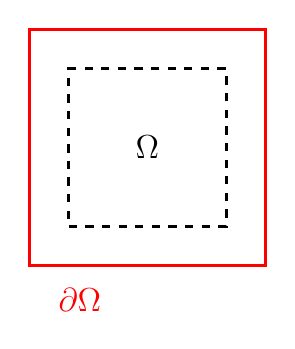
\begin{tikzpicture}[scale=0.5]
    \tikzstyle{every node}=[font=\tiny]
    \draw[style=very thick, color=red] (0,0) node[fill=none, below
      right=1ex,color=red ] { { \large $\partial\Omega$ } } -- (6,0) -- (6,6) --
      (0,6) -- cycle;
    \draw[style=very thick,dashed] (1,1) -- (5,1) -- (5,5) -- (1,5) -- cycle;

    \draw (3,3) node[fill=none] { {\large $\Omega$} };
  \end{tikzpicture}
	\end{center}
  \caption{Eliminated Boundary Nodes}
	\label{fig:ReducedBCs}
\end{figure}


This method, however, can be problematic when using $C^1$ FEs. Consider the
boundary $\partial \Omega = \Gamma_1 \bigcup \Gamma_2$, where $\Gamma_1$ and
$\Gamma_2$ correspond to the vertical and horizontal boundaries, respectively
(see \autoref{fig:SplitBoundary}).  On $\Gamma_1$ we know $u=0$ which implies
$u_y = u_{yy} = 0$ on $\Gamma_1$.  On $\Gamma_2$ we know $u=0$ which implies
$u_x = u_{xx} = 0$ on $\Gamma_2$. Thus, simply setting $u^h = 0$ on the boundary
results in the DoFs corresponding to $u_x,\,u_y,\,u_{xx}$, and $u_{yy}$ not
necessarily being set to zero. Therefore, one must force these DoFs to be zero
too or another scheme must be implemented to deal with this case. However,
setting the appropriate DoFs to zero in this manner requires some analysis of
the problem domain before implementation, which is problematic when one wants to
implement a generalized code. To read more about implementation of boundary
conditions for Hermite type FEs see Remark 2.3.8 in Ciarlet\cite{Ciarlet}. To
avoid this one can implement a Lagrange Multiplier scheme
\cite{Babuska1973,Barbosa1991,Barbosa1992,Bramble1981,Pitkaranta1981}.

\begin{figure}[h]
	\begin{center}
  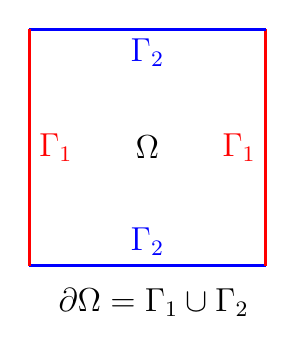
\begin{tikzpicture}[scale=0.5]
    \tikzstyle{every node}=[font=\tiny]
    \draw[style=very thick,color=blue] (0,0)
    node[fill=none, below right=1ex, color=black] { { \large $\partial\Omega = \Gamma_1 \cup \Gamma_2$ } }
    -- (3,0) -- (6,0);
    \draw[style=very thick,color=red] (6,0) -- (6,3) -- (6,6);
    \draw[style=very thick,color=blue] (6,6) -- (3,6) -- (0,6);
    \draw[style=very thick,color=red] (0,6) -- (0,3) -- (0,0);

    \draw (3,3) node[fill=none] { {\large $\Omega$} };
    \draw[color=red] (0,3) node[fill=none,right] { {\large $\Gamma_1$} };
    \draw[color=blue] (3,0) node[fill=none,above] { {\large $\Gamma_2$} };
    \draw[color=red] (6,3) node[fill=none,left] { {\large $\Gamma_1$} };
    \draw[color=blue] (3,6) node[fill=none,below] { {\large $\Gamma_2$} };
  \end{tikzpicture}
	\end{center}
  \caption{Decomposed Boundary}
	\label{fig:SplitBoundary}
\end{figure}


Rewrite the FE formulation, \eqref{eqn:PoissonFE}, in the following way
\begin{equation}
  \begin{split}
    A u &= \ell \\
    \Lambda u &= b,
  \end{split}
  \label{eqn:ConstrainedPoisson}
\end{equation}
where is $\Lambda u = b$ is the constraint equation descibing the boundary
conditions and $A u = \ell$ is the FE formulation of the Poisson equation.
Then the \emph{variational form} of \eqref{eqn:ConstrainedPoisson} is
\begin{equation}
  L(u,\lambda) = \frac{1}{2}u^T A u - u^T \ell + \lambda^T (\Lambda u - b),
  \label{eqn:Variational}
\end{equation}
where $\lambda$ is the Lagrange multiplier. Using the first-order optimality
condition results in
\begin{equation}
  \begin{split}
    \frac{d L}{du} &= Au - \ell + \Lambda^t \lambda = 0 \\
    \frac{d L}{d\lambda} &= \Lambda u - b = 0.
  \end{split}
  \label{eqn:Condition}
\end{equation}
Thus, given $b = \mathbf{0}$ the new system of equations using Lagrange
multipliers for boundary constraints is given by
\begin{equation}
  \begin{bmatrix}
    A & \Lambda^T \\
    \Lambda &  \mathbf{0} \\
  \end{bmatrix} \begin{bmatrix}
    u \\ \lambda
  \end{bmatrix} = \begin{bmatrix}
    \ell \\ \mathbf{0}
  \end{bmatrix}.
  \label{eqn:Lagrange}
\end{equation}
To avoid zeros on the main diagonal, and avoid poor condition of the system
\eqref{eqn:Lagrange}, we add a small perturbation, $\varepsilon$, in the lower
right.

    \section{Two Level Method} \label{sec:TwoLevel}
    Although, the streamfunction formulation of the QGE contains only one flow
variable, $\psi$, it still suffers from
having to solve a large nonlinear system of equations. This is usually done by
using a nonlinear solver, such as Newton's method. These nonlinear solvers
typically require solving large linear systems multiple times to obtain the
solution to the nonlinear system. Solving these large linear systems multiple
times can be time consuming. Thus, a two-level algorithm can improve solve times
greatly over the standard nonlinear sover, since we need only solve the
nonlinear system on a coarse mesh and then use that solution to solve a linear
system on a fine mesh. To this end, this section discusses the two-level
finite element discretization for the pure streamfunction formulation of the
SQGE and QGE.

      \subsection{Two Level Algorithm} \label{sse:Algorithm}
      We consider an approximate solution to \eqref{eqn:SQGEWF} by a two-level finite
element procedure \cite{Fairag98,Layton93}. Let $X^h,\, X^H \subset
H^2_0(\Omega)$ denote two conforming finite element spaces with $H \gg h$. We
compute an approximate solution $\psi^h$ in the finite element space $X^h$ by
solving a linear system consisting of the degrees of freedom in $X^h$.  This
linear system requires us to first compute the approximate solution $\psi^H$ to
the nonlinear system in the finite element space $X^H$ where the mesh is very
coarse, i.e. $H \gg h$ and then using this solution, $\psi^H$, in the linear
system. This procedure is as follows

\begin{algorithm}%[H]
  \caption{}%Two-Level algorithm for the Streamfunction formulation of QGE}
  \label{alg:TwoLevel}
  \begin{enumerate}[Step 1:]
    \item Solve the nonlinear system on a coarse mesh for $\psi^H\in X^H$:
    \begin{equation}
      Re^{-1} (\Delta \psi^H, \Delta \chi^H)
        + b(\psi^H; \psi^H,\chi^H)
        - Ro^{-1} (\psi_x^H,\chi^H)
        = Ro^{-1} (F,\chi^H), \quad \text{for all } \chi^H \in X^H.
      \label{eqn:Coarse}
    \end{equation}
    \item Solve the linear system on a fine mesh for $\psi^h\in X^h$:
    \begin{equation}
      Re^{-1} (\Delta \psi^h, \Delta \chi^h)
        + b(\psi^H; \psi^h,\chi^h)
        - Ro^{-1} (\psi_x^h,\chi^h)
        = Ro^{-1} (F,\chi^h), \quad \text{for all } \chi^h \in X^h.
      \label{eqn:Fine}
    \end{equation}
  \end{enumerate}
\end{algorithm}
\begin{lemma}\label{lma:Fine}
  Given a solution $\psi^H$ of \eqref{eqn:Coarse}, then the solution to the
  following problem exists uniquely
    \begin{equation}
      \begin{split}
        &\text{Find } \hat{\psi} \in H^2_0(\Omega) \text{ such that, for all }
          \chi\in H^2_0(\Omega), \\
        Re^{-1}&(\Delta \hat{\psi}, \Delta \chi)
          + b(\psi^H; \hat{\psi}, \chi)
          - Ro^{-1} (\hat{\psi}_x,\chi)
          = Ro^{-1} (F,\chi),
      \end{split}
      \label{eqn:FineProb}
    \end{equation}
    and satisfies $\|\hat{\psi}\|_2 \le Re\, Ro^{-1} \|F\|_{-2}$.
\end{lemma}
\begin{proof}
  First we introduce a new continuous bilinear form $B:\, H^2_0(\Omega) \times
  H^2_0(\Omega) \to \R$ given by
  \begin{equation*}
    B(\psi,\chi) = Re^{-1} (\Delta \psi, \Delta \chi)
      + b(\psi^H;\psi,\chi)
      - Ro^{-1} (\psi_x,\chi).
  \end{equation*}
  B is continuous and coercive and therefore $\hat{\psi}$ exists and is unique.
  Now setting $\chi=\hat{\psi}$ in \eqref{eqn:FineProb} and noting that
  $(\psi_x,\chi) = -(\chi_x,\psi)$ which implies that
  $(\hat{\psi}_x,\hat{\psi}) = 0$ gives
  \begin{align*}
    Re^{-1} \|\hat{\psi}\|_2^2 &= Ro^{-1} (F,\hat{\psi}) \\
    \|\hat{\psi}\|_2 &= Re\, Ro^{-1} \frac{(F,\hat{\psi})}{\|\hat{\psi}\|_2} \\
    &\le Re\, Ro^{-1} \|F\|_{-2}\|\hat{\psi}\|_2 \\
  \end{align*}
  Therefore, it follows that $\|\hat{\psi}\|_2 \le Re\, Ro^{-1} \|F\|_{-2}$.
\end{proof}
\begin{lemma} \label{lma:Fineh}
  The solution to \eqref{eqn:Coarse} exists and satisfies
  \begin{equation*}
    \|\psi^H\|_2 \le Re\, Ro^{-1} \|F\|_{-2}.
  \end{equation*}
\end{lemma}
\begin{proof}
  The bilinear form $B$ is continuous and coercive on $X^h$ and so $\psi^h$
  exists and is unique. Setting, $\chi^h=\psi^h$ in \eqref{eqn:Fine} and again
  noting that $(\psi_x^h,\psi^h)=0$ and using \eqref{eqn:lCont} gives
  \begin{align*}
    Re^{-1} \|\psi^h\|_2^2 &= Ro^{-1} (F,\psi^h) \\
    \|\psi^h\|_2 &= Re Ro^{-1} \frac{(F,\psi^h)}{\|\psi^h\|_2} \\
    &\le Re\, Ro^{-1} \|F\|_{-2}.
  \end{align*}
\end{proof}

    %\section{Method of Lines} \label{sec:MoL}
    %The \emph{method of lines} refers to the application of the \emph{finite
difference} method to a semi-discretization of an equation, i.e. the spatial
domain has been discretized by the finite element method and then the time
domain is discretized using a finite difference method. This is the preferable
method for discretization of the time domain, due to its simplicity and the fact
that the time domain does not have geometry.

In particular, we may apply a a \emph{backward Euler} finite difference scheme
to \eqref{eqn:SemiDiscretization} which would produce the following
discretization of the streamfunction form of the QGE
\begin{equation}
  a_0(\psi_h^{n+1} - \psi_h^n, \chi_h) + k\, \left[a_1(\psi_h^n,\chi_h) + b(\psi_h^n,\psi_h^n,\chi_h)
      + (\psi_x_h^n,\chi_h)\right] = k\, \ell^n(\chi_h),\quad \forall \, \chi_h \in X^h.
  \label{eqn:BEQGE}
\end{equation}
where $k$ is the time step, subscripts represent the discretization in spatial
domains, and superscripts represent the discretization in time domain.
Additionally, fince the linear form $(F,\chi_h)$ is, in fact, time dependent
we place a superscript to indicate the discretization of the $\ell$ in the time
domain.  The attractiveness of using this backward Euler scheme is that it is
explicit and therefore one need not solve the nonlinear system that would arize
from the \emph{forward Euler} scheme. However, it is well known that the
backward Euler scheme is not a-stable and therefore one needs to be careful to
satisfy a CFL type condition.

Here in lies the problem with using a high order finite element scheme, such as
the Argyris element, and the method of lines; the backward Euler scheme is first
order in time whereas the Argyris element is sixth order in the $L^2$ norm.
Thus, we might expect a CFL condition of the form
\begin{equation*}
  \frac{k}{h^6} \le C
\end{equation*}
where $C$ is a dimensionless constant that does not depend on either $k$ or $h$.
Thus, we might expect to need quite a small time step, which may be unreasonably
small for numerical simulations.  Therefore, either a higher order finite
difference scheme will need to be used, or an explicit finite difference scheme
will need to be employed.

While an implicit scheme might seem an attactive option, one must take into
account the ammount of time required to solve the nonlinear system at each time
step. For larger spatial discretizations the time to solve such nonlinear
systems might be prohibitive. Therefore, higher order finite difference schemes
appear to be the more attractive approach.

However, there may be hope for the explicit finite element schemes after all. It
might be possible to apply the two-level method (\autoref{alg:TwoLevel}) to the
QGE at each time step. That is we solve the nonlinear system on a coarse mesh
and then use that solution to linearize the nonlinear system on the fine mesh.
This method may allow for much quicker calculations than might be expected using
just an explicit finite difference scheme alone. We expect that this method will
produce good results.


  \chapter{Error Analysis} \label{ch:Errors}
  The main goal of this Chapter is to develop rigorous numerical analysis for
the FE discritezation of the QGE \eqref{eqn:QGE_psi} for a conforming FE
discretization. In particular we focus on the use of the Argyris element, but
the majority of the results apply to any conforming FE discretization of QGE
\eqref{eqn:QGE_psi}, SQGE \eqref{eqn:SQGE_Psi}, and the two-level method applied
to SQGE \eqref{eqn:SQGE_Psi}.

In the sections that follow we rely heavily on the Young inequality, H\"older
inequality , Cauchy-Schwarz inequality, Poincar\'e-Friedrich inequality, and
Ladyzenskya inequality, so for completeness we will state them here.

\begin{definition} \label{def:Young}
  \textbf{Young inequality} \cite{Royden2010}:\\
  For $1 < p,q < \infty$, $\dfrac{1}{p} + \dfrac{1}{q} = 1$, and any two
  positive numbers $a$ and $b$,
  \begin{equation}
    ab \le \frac{a^p}{p} + \frac{b^q}{q}
    \label{eqn:Young}
  \end{equation}
\end{definition}
\begin{definition} \label{def:Holder}
  \textbf{H\"older inequality} \cite{Royden2010}:\\
  Let $\Omega$ be a measurable set, $1\le p,q < \infty$, and $\dfrac{1}{p} +
  \dfrac{1}{q} = 1$. If $f \in L^p(\Omega)$ and $g \in L^q(\Omega)$, then their
  product $f\cdot g$ is integrable over $\Omega$ and
  \begin{equation}
    \int_{\Omega}\! |f\cdot g| \, d\mathbf{x} \le \|f\|_p\, \|g\|_q.
    \label{eqn:Holder}
  \end{equation}
\end{definition}
\begin{definition} \label{def:Cauchy-Schwarz}
  \textbf{Cauchy-Schwarz inequality} \cite{Royden2010}:\\
  Let $\Omega$ be a measurable set and $f$ and $g$ be square-integrable over
  $\Omega$. Then their product $f\cdot g$ is also over $\Omega$ and
  \begin{equation}
    \int_{\Omega}\! |f\,g|\, d\mathbf{x} \le \sqrt{\int_{\Omega}\! f^2 \,
      d\mathbf{x}} \cdot \sqrt{\int_{\Omega}\! g^2 \, d\mathbf{x}}
    \label{eqn:Cauchy}
  \end{equation}

\end{definition}
\begin{definition} \label{def:Poincare}
  \textbf{Poincar\'e-Friedrich inequality} \cite{Layton08}:\\
  Let $\Omega$ be a measurable set and $u \in H^1_0(\Omega)$. Then there is a
  positive constant $C_P = C_P(\Omega)$ such that
  \begin{equation}
    \|u\| \le C_P \|\nabla u\| \quad \forall u \in X
    \label{eqn:Poincare}
  \end{equation}
\end{definition}
\begin{definition} \label{def:Ladyzhenskaya}
  \textbf{Ladyzhenskaya inequality \cite{Layton08}:}\\
  For any vector function $u\,:\, \R^2 \rightarrow \R^2$ with compact support
  and with the indicated finite $L^4$ and $L^2$ norms,
  \begin{equation}
    \|u\|_{L^4(\R^2)} \le 2^{\nicefrac{1}{4}}
      \|u\|^{\nicefrac{1}{2}}_{L^2(\R^2)}
      \|\nabla u\|^{\nicefrac{1}{2}}_{L^2(\R^2)}
    \label{eqn:Ladyzhenskaya}
  \end{equation}
\end{definition}
With these definitions we can now proceed with the error analysis.

    \section{SQGE} \label{sec:SQGEErrors}
    The main goal of this section is to develop a rigorous numerical analysis for the FEM discretization
of the QGE \eqref{eqn:SQGEFEF} by using the conforming Argyris element.  First, in
Theorem~\ref{thm:EnergyNorm} we prove error estimates in the $H^2$ norm by using an approach similar
to that used in \cite{Cayco86}.  Second, in Theorem~\ref{thm:Errors}, we prove error estimates in
the $L^2$ and $H^1$ norms by using a duality argument.

\begin{thm}
\label{thm:EnergyNorm}
  Let $\psi$ be the solution of \eqref{eqn:SQGEWF} and $\psi^h$ be the solution
  of \eqref{eqn:SQGEFEF}.
  Furthermore, assume that the following small data condition is satisfied:
  \begin{eqnarray}
  Re^{-2} \, Ro
  \geq \Gamma_1 \, \| F \|_{-2} ,
  \label{eqn:small_data_condition}
  \end{eqnarray}
where
$Re$ is the Reynolds number defined in \eqref{eqn:reynolds_number},
$Ro$  is the Rossby number defined in \eqref{eqn:rossby_number},
 $\Gamma_1$ is the continuity constant of the trilinear form $a_2$ in \eqref{eqn:a2Cont}, and
 $F$ is the forcing term.
Then the following error estimate holds:
  \begin{equation}
    |\psi - \psi^h|_2
    \le C(Re, Ro, \Gamma_1, F) \, \inf_{\chi^h \in X^h} |\psi - \chi^h|_2 ,
    \label{eqn:EnergyNorm}
  \end{equation}
  where
  \begin{eqnarray}
  C(Re, Ro, \Gamma_1, F)
  := \left[
  \frac{
  Ro^{-1}
  + 2 \, Re^{-1}
  + \Gamma_1 \, Re \, Ro^{-1} \, \| F \|_{-2}
  }
  {
  Re^{-1}
  - \Gamma_1 \, Re \, Ro^{-1} \, \| F \|_{-2}
  }
  \right]
  \label{eqn:constant_definition}
  \end{eqnarray}
is a generic constant that can depend on $Re$, $Ro$, $\Gamma_1$, $F$, but \emph{not} on the meshsize $h$.
\end{thm}

\begin{remark}
Note that the small data condition in Theorem~\ref{thm:EnergyNorm} involves \emph{both} the Reynolds number and the Rossby number, the latter quantifying the rotation effects in the QGE.

Furthermore, note that the standard small data condition $Re^{-2} \geq \Gamma_1 \, \| F \|_{-2}$ used to prove the uniqueness for the steady-state 2D NSE \cite{Girault79,Girault86,Layton08} is significantly more restrictive for the QGE, since \eqref{eqn:small_data_condition} has the Rossby number (which is small when rotation effects are significant) on the left-hand side.
This is somewhat counterintuitive, since in general rotation effects are expected to help in proving the well-posedness of the system.
We think that the explanation for this puzzling situation is the following:
Rotation effects do make the mathematical analysis of 3D flows more amenable by giving them a 2D character.
We, however, are concerned with 2D flows (the QGE).
In this case, the small data condition \eqref{eqn:small_data_condition} (needed in proving the uniqueness of the solution) indicates that rotation effects make the mathematical analysis of the (2D) QGE more complicated than that of the 2D NSE.
%We emphasize that there is no contradiction, since, although the rotation effects do help in the three-dimensional case, they seem to complicate the situation if one compare the QGE with the two-dimensional (not the three-dimensional) NSE.
\end{remark}
\begin{proof}
  Since $X^h \subset X$, \eqref{eqn:SQGEWF} holds for all $\chi = \chi^h\in X^h$.
  Subtracting \eqref{eqn:SQGEFEF} from \eqref{eqn:SQGEWF} with $\chi=\chi^h \in
  X^h$ gives
  \begin{equation}
    \begin{split}
      a_1(\psi - \psi^h,\chi^h) + a_2(\psi,\psi,\chi^h) -
      a_2(\psi^h,\psi^h,\chi^h) \\
      + a_3(\psi-\psi^h,\chi^h) = 0 \qquad \forall \chi^h \in
    X^h.
  \end{split}
    \label{eqn:ErrorEq}
  \end{equation}
  Next, adding and subtracting $a_2(\psi^h,\psi,\chi^h)$ to \eqref{eqn:ErrorEq}, we get:
  \begin{eqnarray}
    %\begin{split}
      && a_1(\psi - \psi^h,\chi^h) + a_2(\psi,\psi,\chi^h) - a_2(\psi^h,\psi,\chi^h) %\\
      + a_2(\psi^h,\psi,\chi^h) - a_2(\psi^h,\psi^h,\chi^h) \nonumber \\
      && \hspace*{3.0cm} + a_3(\psi-\psi^h,\chi^h) = 0 \qquad \forall \chi^h \in X^h.
    %\end{split}
    \label{eqn:interError}
  \end{eqnarray}
  The error $e$ can be decomposed as
  \begin{equation}
    e:= \psi-\psi^h = (\psi-\lambda^h)+(\lambda^h-\psi^h):= \eta + \Phi^h,
    \label{eqn:ErrorTrick}
  \end{equation}
  where $\lambda^h\in X^h$ is arbitrary.
  Thus, equation \eqref{eqn:interError} can be
  rewritten as
  \begin{equation}
    \begin{split}
      a_1(\eta+\Phi^h,\chi^h)+a_2(\eta+\Phi^h,\psi,\chi^h)+a_2(\psi^h,\eta+\Phi^h,\chi^h) \\
      + a_3(\eta+\Phi^h,\chi^h)=0 \qquad \forall \chi^h \in X^h.
    \end{split}
    \label{eqn:ErrorEta}
  \end{equation}
  Letting $\chi^h := \Phi^h$ in \eqref{eqn:ErrorEta}, we obtain
  \begin{equation}
    \begin{split}
      a_1(\Phi^h,\Phi^h) + a_3(\Phi^h,\Phi^h) = -a_1(\eta,\Phi^h)
      - a_2(\eta;\psi,\Phi^h) - a_2(\psi^h;\psi,\Phi^h) \\
      - a_2(\psi^h;\eta,\Phi^h) - a_2(\psi^h;\Phi^h,\Phi^h)
      -a_3(\eta,\Phi^h).
    \end{split}
    \label{eqn:ErrorVarphi}
  \end{equation}
  Note that, since $a_3(\Phi^h,\Phi^h)=-a_3(\Phi^h,\Phi^h)\; \forall
  \Phi^h \in X^h \subset X = H^2_0$, it follows that
  \begin{equation}
    a_3(\Phi^h,\Phi^h)=0 .
    \label{eqn:a30}
  \end{equation}
  Also, it follows immediately from \eqref{eqn:a2} that
  \begin{equation}
    a_2(\psi^h,\Phi^h,\Phi^h)=0 .
    \label{eqn:a20}
  \end{equation}
  Combining \eqref{eqn:a20}, \eqref{eqn:a30}, and \eqref{eqn:ErrorVarphi}, we get:
  \begin{equation}
    \begin{split}
      a_1(\Phi^h,\Phi^h) = -a_1(\eta,\Phi^h)
      - a_2(\Phi^h;\psi,\Phi^h) - a_2(\eta;\psi,\Phi^h) \\
      - a_2(\psi^h;\eta,\Phi^h) - a_3(\eta,\Phi^h).
    \end{split}
    \label{eqn:ErrorZeroed}
  \end{equation}
  Using
  \begin{equation*}
    a_1(\Phi^h,\Phi^h) = Re^{-1} \, |\Phi^h|^2_2
  \end{equation*}
  and inequalities \eqref{eqn:a1Cont} -- \eqref{eqn:a3Cont} in equation
  \eqref{eqn:ErrorZeroed} gives
  \begin{equation}
    \begin{split}
      Re^{-1} \, |\Phi^h|^2_2 \le Re^{-1} \,  |\eta|_2 \, |\Phi^h|_2 + \Gamma_1
      \biggl( |\eta|_2 \, |\psi|_2 \, |\Phi^h|_2 + |\psi^h|_2 \, |\eta|_2 \, |\Phi^h|_2 \biggr) \\
      + \Gamma_1 \, |\Phi^h|^2_2 \, |\psi|_2 + Ro^{-1} \, |\eta|_2 \, |\Phi^h|_2 .
    \end{split}
    \label{eqn:varphiIneq}
  \end{equation}
  Simplifying and rearranging terms in \eqref{eqn:varphiIneq} gives
  \begin{equation}
      |\Phi^h|_2
      \le
      \left(
      Re^{-1}
      - \Gamma_1 \, | \psi |_2
      \right)^{-1} \,
      \left(
      Re^{-1}
      + \Gamma_1 \, |\psi|_2
      + \Gamma_1 \, |\psi^h|_2
      + Ro^{-1}
      \right) \,
      |\eta|_2 .
    \label{eqn:phihIneq}
  \end{equation}
  Using \eqref{eqn:phihIneq} and the triangle inequality along with the stability estimates \eqref{eqn:stability_sqge} and \eqref{eqn:stability_fem_sqge} gives
  \begin{align}
    |e|_2
    &\le |\eta|_2
    + |\Phi^h|_2 \nonumber \\[0.2cm]
    &\le \left[
    1
    + \frac{Re^{-1}
      + \Gamma_1 \, |\psi|_2
      + \Gamma_1 \, |\psi^h|_2
      + Ro^{-1}} {Re^{-1}
      - \Gamma_1 \, |\psi|_2}
      \right] \, |\eta|_2 \nonumber \\[0.2cm]
    &\le \left[
    1
    + \frac{Re^{-1}
      + \Gamma_1 \, \left( Re \, Ro^{-1} \, \| F \|_{-2} \right)
      + \Gamma_1 \, \left( Re \, Ro^{-1} \, \| F \|_{-2} \right)
      + Ro^{-1}} {Re^{-1}
      - \Gamma_1 \, \left( Re \, Ro^{-1} \, \| F \|_{-2} \right) }
      \right] \, |\eta|_2 \nonumber \\
  &=
  \left[
  \frac{
  Ro^{-1}
  + 2 \, Re^{-1}
  + \Gamma_1 \, Re \, Ro^{-1} \, \| F \|_{-2}
  }
  {
  Re^{-1}
  - \Gamma_1 \, Re \, Ro^{-1} \, \| F \|_{-2}
  }
  \right] \, | \psi-\lambda^h |_2 ,
    \label{eqn:EnergyError}
  \end{align}
where $\lambda^h \in X^h$ is arbitrary.
Taking the infimum over $\lambda^h \in X^h$ in \eqref{eqn:EnergyError} proves the error estimate \eqref{eqn:EnergyNorm}.
\hfill
\end{proof}

In Theorem~\ref{thm:EnergyNorm}, we proved an error estimate in the $H^2$ norm.
In Theorem~\ref{thm:Errors}, we will prove error estimates in the $L^2$ and $H^1$ norms by using a duality argument.
To this end, we first notice that the QGE \eqref{eqn:QGE_psi} can be written as
\begin{eqnarray}
\mathcal{N} \, \psi
= Ro^{-1} \, F ,
\label{eqn:qge_operator_formulation}
\end{eqnarray}
where the nonlinear operator $\mathcal{N}$ is defined as
\begin{eqnarray}
\mathcal{N} \, \psi
:= Re^{-1} \, \Delta^2 \psi
+ J(\psi , \Delta \psi)
- Ro^{-1} \, \frac{\partial \psi}{\partial x} .
\label{eqn:nonlinear_operator}
\end{eqnarray}
The linearization of $\mathcal{N}$ around $\psi$, a solution of \eqref{eqn:QGE_psi}, yields the following \emph{linear} operator:
\begin{eqnarray}
\mathcal{L} \, \chi
:= Re^{-1} \, \Delta^2 \chi
+ J(\chi , \Delta \psi)
+ J(\psi, \Delta \chi)
- Ro^{-1} \, \frac{\partial \chi}{\partial x} .
\label{eqn:linear_operator}
\end{eqnarray}
To find the dual problem associated with the QGE \eqref{eqn:qge_operator_formulation}, we first define the \emph{dual operator} $\mathcal{L}^*$ of $\mathcal{L}$:
\begin{eqnarray}
(\mathcal{L} \, \chi , \psi^*)
= ( \chi , \mathcal{L}^* \, \psi^*)
\qquad
\forall \, \psi^* \in X .
\label{eqn:dual_operator}
\end{eqnarray}
To find $\mathcal{L}^*$, we use the standard procedure:
In \eqref{eqn:dual_operator}, we use the definition of $\mathcal{L}$ given in \eqref{eqn:linear_operator} and we ``integrate by parts" (i.e., use Green's theorem):
\begin{eqnarray}
\hspace*{-0.4cm}
(\mathcal{L} \, \chi , \psi^*)
&=& \left(
Re^{-1} \, \Delta^2 \chi
+ J(\chi , \Delta \psi)
+ J(\psi, \Delta \chi)
- Ro^{-1} \, \frac{\partial \chi}{\partial x}
\, , \, \psi^*
\right)
\nonumber \\
&=& \left(
\chi \, , \,
Re^{-1} \, \Delta^2 \, \psi^*
- J(\psi , \Delta \psi^* )
+ Ro^{-1} \, \frac{\partial \psi^*}{\partial x}
\right)
+ \biggl( J(\chi , \Delta \psi) , \psi^* \biggr) ,
\label{eqn:dual_operator_1}
\end{eqnarray}
where to get the first term on the right-hand side of \eqref{eqn:dual_operator_1} we used the skew-symmetry of the trilinear form $a_2$ in the last two variables and Green's theorem (just as we did in the proof of Theorem \ref{thm:stability_sqge}).
Next, we apply Green's theorem to the second term on the right-hand side of \eqref{eqn:dual_operator_1}:
\begin{eqnarray}
\biggl( J(\chi , \Delta \psi) , \psi^* \biggr)
&=& \chi_x \, \Delta \psi_y \, \psi^*
   -    \chi_y \, \Delta \psi_x \, \psi^*
\nonumber \\
&\stackrel{Green}{=}&
- \chi \, \Delta \psi_{y x} \, \psi^*
- \chi \, \Delta \psi_y \, \psi^*_x
+ \chi \, \Delta \psi_{x y} \, \psi^*
+ \chi \, \Delta \psi_x \, \psi^*_y
\nonumber \\
&=& \biggl( \chi , J(\Delta \psi , \psi^*) \biggr) .
\label{eqn:dual_operator_2}
\end{eqnarray}
Equations \eqref{eqn:dual_operator_1}-\eqref{eqn:dual_operator_2} imply:
\begin{eqnarray}
(\mathcal{L} \, \chi , \psi^*)
&=& \left(
\chi \, , \,
Re^{-1} \, \Delta^2 \, \psi^*
- J(\psi , \Delta \psi^* )
+ Ro^{-1} \, \frac{\partial \psi^*}{\partial x}
\right)
+ \biggl( \chi , J(\Delta \psi , \psi^*) \biggr)
\nonumber \\
&=& ( \chi , \mathcal{L}^* \, \psi^*) .
\label{eqn:dual_operator_3}
\end{eqnarray}
Thus, the \emph{dual operator} $\mathcal{L}^*$ is given by
\begin{eqnarray}
\mathcal{L}^* \, \psi^*
= Re^{-1} \, \Delta^2 \, \psi^*
- J(\psi , \Delta \psi^* )
+ J(\Delta \psi , \psi^* )
+ Ro^{-1} \, \frac{\partial \psi^*}{\partial x} .
\label{eqn:dual_operator_4}
\end{eqnarray}
For any given $g \in L^2(\Omega)$, the weak formulation of the \emph{dual problem} is:
\begin{eqnarray}
( \mathcal{L}^* \, \psi^* , \chi )
= (g , \chi)
\qquad
\forall \, \chi \in X = H_0^2(\Omega) .
\label{eqn:dual_operator_5}
\end{eqnarray}
We assume that $\psi^*$, the solution of \eqref{eqn:dual_operator_5}, satisfies the following elliptic regularity estimates:
\begin{eqnarray}
&& \psi^* \in H^4(\Omega) \cap H^2_0(\Omega),
\label{eqn:dual_operator_6a} \\[0.2cm]
&& \| \psi^* \|_4
\le C \, \|g\|_{0},
\label{eqn:dual_operator_6b} \\[0.2cm]
&& \| \psi^* \|_3
\le C \, \|g\|_{-1},
\label{eqn:dual_operator_6c}
\end{eqnarray}
where $C$ is a generic constant that can depend on the data, but not on the meshsize $h$.
\begin{remark}
We note that this type of elliptic regularity was also assumed in \cite{Cayco86} for the streamfunction formulation of the 2D NSE.
In that report, it was also noted that for a polygonal domain satisfying a minimum angle condition, Rannacher et al. \cite{} had actually proved this elliptic regularity.
\end{remark}

The error estimates in the $L^2$ and $H^1$ norms that we prove in Theorem~\ref{thm:Errors} are
derived for the particular space $X^h\subset H^2_0(\Omega)$ consisting of Argyris elements, although
the same results can be derived for other conforming $C^1$ finite element spaces.
\begin{thm} \label{thm:Errors}
  Let $\psi$ be the solution of \eqref{eqn:SQGEWF} and $\psi^h$ be the solution
  of \eqref{eqn:SQGEFEF}.
  Assume that the same small data condition as in Theorem \ref{thm:EnergyNorm} is satisfied:
  \begin{eqnarray}
  Re^{-2} \, Ro
  \geq \Gamma_1 \, \| F \|_{-2} .
  \label{eqn:small_data_condition_dual}
  \end{eqnarray}
  Furthermore, assume that $\psi\in H^6(\Omega) \cap H^2_0(\Omega)$.
  Then there exist positive constants $C_0, \, C_1 \text{ and } C_2$ that can depend on $Re$, $Ro$, $\Gamma_1$, $F$, but \emph{not} on the meshsize $h$, such that
  \begin{align}
    |\psi - \psi^h|_2 &\le C_2 \, h^4 , \label{eqn:H2Error} \\
    |\psi - \psi^h|_1 &\le C_1 \, h^5 , \label{eqn:H1Error} \\
    \|\psi - \psi^h\|_0 &\le C_0 \, h^6 . \label{eqn:L2Error}
  \end{align}
\end{thm}
\begin{proof}
Estimate \eqref{eqn:H2Error} follows immediately from \eqref{eqn:argyris_approximation_0} and Theorem \ref{thm:EnergyNorm}.
Estimates \eqref{eqn:L2Error} and \eqref{eqn:H1Error} follow from a duality argument.

The error in the primal problem \eqref{eqn:SQGEWF} and the interpolation error in the dual problem  \eqref{eqn:dual_operator_5} are denoted as
\begin{eqnarray}
e
:= \psi
- \psi^h
\qquad
e^*
: = \psi^*
- {\psi^*}^h ,
\label{eqn:theorem_dual_1}
\end{eqnarray}
respectively.

We start proving the $L^2$ norm estimate \eqref{eqn:L2Error}.
\begin{eqnarray}
|e|^2
= (e , e)
&=& (\mathcal{L} \, e , \psi^*)
= (e , \mathcal{L}^* \, \psi^*)
\nonumber \\
&=& (e , \mathcal{L}^* \, e^*)
+ (e , \mathcal{L}^* \, {\psi^*}^h)
= (\mathcal{L} \, e , e^*)
+ (\mathcal{L} \, e , {\psi^*}^h) .
\label{eqn:theorem_dual_2}
\end{eqnarray}
The last term on the right-hand side of \eqref{eqn:theorem_dual_2} is given by
\begin{eqnarray}
(\mathcal{L} \, e , {\psi^*}^h)
= \left(
Re^{-1} \, \Delta^2 e
+ J(e , \Delta \, \psi)
+ J(\psi , \Delta \, e)
- Ro^{-1} \, \frac{\partial e}{\partial x}
 \, , \,
{\psi^*}^h
\right) .
\label{eqn:theorem_dual_3}
\end{eqnarray}
To estimate this term, we consider the error equation obtained by subtracting \eqref{eqn:SQGEFEF} (with $\psi^h= {\psi^*}^h$) from \eqref{eqn:SQGEWF} (with $\chi = {\psi^*}^h$):
\begin{eqnarray}
\left(
Re^{-1} \, \Delta^2 e
- Ro^{-1} \, \frac{\partial e}{\partial x}
 \, , \,
{\psi^*}^h
\right)
+ \left(
 J(\psi , \Delta \, \psi)
- J(\psi^h , \Delta \, \psi^h)
 \, , \,
{\psi^*}^h
\right)
= 0 .
\label{eqn:theorem_dual_4}
\end{eqnarray}
Using \eqref{eqn:theorem_dual_4}, equation \eqref{eqn:theorem_dual_3} can be written as follows:
\begin{eqnarray}
(\mathcal{L} \, e , {\psi^*}^h)
= \left(
 J(e , \Delta \, \psi)
+ J(\psi , \Delta \, e)
- J(\psi , \Delta \, \psi)
+ J(\psi^h , \Delta \, \psi^h)
 \, , \,
{\psi^*}^h
\right) .
\label{eqn:theorem_dual_5}
\end{eqnarray}
Thus, by using \eqref{eqn:theorem_dual_5} equation \eqref{eqn:theorem_dual_2} becomes:
\begin{eqnarray}
|e|^2
&=& (\mathcal{L} \, e , e^*)
+ (\mathcal{L} \, e , {\psi^*}^h)
\nonumber \\
&=& Re^{-1} \, (\Delta e , \Delta e^*)
- Ro^{-1} \, \left( \frac{\partial e}{\partial x} , e^* \right)
+ \left(
J(e , \Delta \psi)
+ J(\psi , \Delta e)
, e^*
\right)
\nonumber \\
&+& \left(
 J(e , \Delta \, \psi)
+ J(\psi , \Delta \, e)
- J(\psi , \Delta \, \psi)
+ J(\psi^h , \Delta \, \psi^h)
 \, , \,
{\psi^*}^h
\right)
\nonumber \\
&=& a_1(e , e^*)
+ a_3(e , e^*)
+ a_2(e , \psi , e^*)
+ a_2(\psi , e, e^*)
+ a_2(e , \psi , {\psi^*}^h)
\nonumber \\
&& - a_2(\psi , \psi , e^*)
+ a_2(\psi^h , \psi^h , e^*)
\nonumber \\
&=& a_1(e , e^*)
+ a_3(e , e^*)
+ a_2(e , \psi , e^*)
+ a_2(\psi , e, e^*)
\nonumber \\
&& - a_2(e , \psi , e^*)
+ a_2(e , \psi^h , e^*)
+ a_2(e , e , \psi^*)
\label{eqn:theorem_dual_6}
\end{eqnarray}
Using the bounds in \eqref{eqn:a1Cont}-\eqref{eqn:a3Cont}, \eqref{eqn:theorem_dual_6} yields:
\begin{eqnarray}
|e|^2
&=& a_1(e , e^*)
+ a_3(e , e^*)
+ a_2(e , \psi , e^*)
+ a_2(\psi , e, e^*)
\nonumber \\
&& - a_2(e , \psi , e^*)
+ a_2(e , \psi^h , e^*)
+ a_2(e , e , \psi^*)
\nonumber \\
&\leq& Re^{-1} \, | e |_2 \, |e^* |_2
+ Ro^{-1} \, | e |_2 \, |e^* |_2
+ \Gamma_1 \, | e |_2 \, | \psi |_2 \, | e^* |_2
+ \Gamma_1 \, | \psi |_2 \, | e |_2 \, | e^* |_2
\nonumber \\
&& + \Gamma_1 \, | e |_2 \, | \psi |_2 \, | e^* |_2
+ \Gamma_1 \, | e |_2 \, | \psi^h |_2 \, | e^* |_2
+ \Gamma_1 \, | e |_2 \, | e |_2 \, | \psi^* |_2
\nonumber \\
&=& | e |_2 \, |e^* |_2 \,
\left(
Re^{-1}
+ Ro^{-1}
+ \Gamma_1 \, | \psi |_2
+ \Gamma_1 \, | \psi |_2
+ \Gamma_1 \, | \psi |_2
+ \Gamma_1 \, | \psi^h |_2
\right)
\nonumber \\
&& + | e |_2^2 \,
\left(
\Gamma_1 \, | \psi^* |_2
\right) .
\label{eqn:theorem_dual_7}
\end{eqnarray}
We start bounding the terms on the right-hand side of \eqref{eqn:theorem_dual_7}.
First, we note that using the stability estimates \eqref{eqn:stability_sqge} for $\psi$ and \eqref{eqn:stability_fem_sqge} for $\psi^h$, the right-hand side of \eqref{eqn:theorem_dual_7} can be bounded as follows:
\begin{eqnarray}
|e|^2
\leq C \, | e |_2 \, |e^* |_2
+ | e |_2^2 \,
\left(
\Gamma_1 \, | \psi^* |_2
\right) ,
\label{eqn:theorem_dual_8}
\end{eqnarray}
where $C$ is a generic constant that can depend on $Re$, $Ro$, $\Gamma_1$, $F$, but \emph{not} on the meshsize $h$.
By using the approximation results \eqref{eqn:argyris_approximation_1}, we get:
\begin{eqnarray}
|e^* |_2
\leq C \, h^2 \, | \psi^* |_4 .
\label{eqn:theorem_dual_9}
\end{eqnarray}
By using \eqref{eqn:dual_operator_6a} and \eqref{eqn:dual_operator_6b}, the elliptic regularity results of the dual problem \eqref{eqn:dual_operator_5} with $g := e$, we also get:
\begin{eqnarray}
| \psi^* |_4
\leq C \, | e | ,
\label{eqn:theorem_dual_10}
\end{eqnarray}
which obviously implies
\begin{eqnarray}
| \psi^* |_2
\leq C \, | e | .
\label{eqn:theorem_dual_11}
\end{eqnarray}
Inequalities \eqref{eqn:theorem_dual_9}-\eqref{eqn:theorem_dual_10} imply:
\begin{eqnarray}
|e^* |_2
\leq C \, h^2 \, | e | .
\label{eqn:theorem_dual_12}
\end{eqnarray}
Inserting \eqref{eqn:theorem_dual_11} and \eqref{eqn:theorem_dual_12}  in \eqref{eqn:theorem_dual_8}, we get:
\begin{eqnarray}
|e|^2
\leq C \, h^2 \, | e |_2 \, | e |
+ C \, | e |_2^2 \, | e | .
\label{eqn:theorem_dual_13}
\end{eqnarray}
Using the obvious simplifications and the $H^2$ error estimate \eqref{eqn:H2Error} in \eqref{eqn:theorem_dual_13} yields:
\begin{eqnarray}
|e|
\leq C \, h^2 \, | e |_2
+ C \, | e |_2^2
\leq C \, h^6 + C \, h^8
= C_0 \, h^6 ,
\label{eqn:theorem_dual_14}
\end{eqnarray}
which proves the $L^2$ error estimate \eqref{eqn:L2Error}.

%\textcolor{blue}{Traian: Check the rest of the proof!!!}

Next, we prove the $H^1$ norm estimate \eqref{eqn:H1Error}.
Since the duality approach we use is similar to that we used in proving the  $L^2$ norm estimate \eqref{eqn:L2Error}, we only highlight the main differences.
We start again by writing the $H^1$ norm of the error in terms of the dual operator $\mathcal{L}^*$:
\begin{eqnarray}
|e|_1^2
&=& (\nabla e , \nabla e)
= ( e , - \Delta e)
= (\mathcal{L} \, e , \psi^*)
= (e , \mathcal{L}^* \, \psi^*)
\nonumber \\
&=& (e , \mathcal{L}^* \, e^*)
+ (e , \mathcal{L}^* \, {\psi^*}^h)
= (\mathcal{L} \, e , e^*)
+ (\mathcal{L} \, e , {\psi^*}^h) .
\label{eqn:theorem_dual_15}
\end{eqnarray}
Thus, the second and fourth equalities in \eqref{eqn:theorem_dual_15} clearly indicate that in the dual problem \eqref{eqn:dual_operator_5}, one should choose $g = - \Delta e$, and not $g = e$, as we did in \eqref{eqn:theorem_dual_10}, when we proved the $L^2$ error estimate \eqref{eqn:L2Error}.
Using \eqref{eqn:dual_operator_6a} and \eqref{eqn:dual_operator_6c}, the elliptic regularity results of the dual problem \eqref{eqn:dual_operator_5} with $g :=  - \Delta e$, we also get:
\begin{eqnarray}
| \psi^* |_3
\leq C \, | - \Delta e |_{-1}
\leq C \, | e |_1 ,
\label{eqn:theorem_dual_16}
\end{eqnarray}
where in the last inequality we used the fact that $e \in H_0^2(\Omega)$.
Inequality \eqref{eqn:theorem_dual_16} obviously implies
\begin{eqnarray}
| \psi^* |_2
\leq C \, | e |_1 .
\label{eqn:theorem_dual_17}
\end{eqnarray}
All the results in \eqref{eqn:theorem_dual_3}-\eqref{eqn:theorem_dual_7} carry over to our setting.
%\textcolor{blue}{Traian: Check !!!}
Thus, we get:
\begin{eqnarray}
|e|_1^2
\leq C \, | e |_2 \, |e^* |_2
+ C \, | e |_2^2 \, | \psi^* |_2 ,
\label{eqn:theorem_dual_18}
\end{eqnarray}
where $C$ is a generic constant that can depend on $Re$, $Ro$, $\Gamma_1$, $F$, but \emph{not} on the meshsize $h$.
By using the approximation result \eqref{eqn:argyris_approximation_2}, we get:
\begin{eqnarray}
|e^* |_2
\leq C \, h \, | \psi^* |_3 .
\label{eqn:theorem_dual_19}
\end{eqnarray}
Inequalities \eqref{eqn:theorem_dual_19}-\eqref{eqn:theorem_dual_16} imply:
\begin{eqnarray}
|e^* |_2
\leq C \, h \, | e |_1 .
\label{eqn:theorem_dual_20}
\end{eqnarray}
Inserting \eqref{eqn:theorem_dual_17} and \eqref{eqn:theorem_dual_20}  in \eqref{eqn:theorem_dual_18}, we get:
\begin{eqnarray}
|e|_1^2
\leq C \, h \, | e |_2 \, | e |_1
+ C \, | e |_2^2 \, | e |_1 .
\label{eqn:theorem_dual_21}
\end{eqnarray}
Using the obvious simplifications and the $H^2$ error estimate \eqref{eqn:H2Error} in \eqref{eqn:theorem_dual_21} yields:
\begin{eqnarray}
|e|_1
\leq C \, h \, | e |_2
+ C \, | e |_2^2
\leq C \, h^5 + C \, h^8
= C_1 \, h^5 ,
\label{eqn:theorem_dual_22}
\end{eqnarray}
which proves the $H^1$ error estimate \eqref{eqn:H1Error}.
%\vspace*{4.0cm}
\hfill
\end{proof}

    \section{Two Level Method} \label{sse:SQGE2LE}
    The main goal of this section is to develop a rigorous numerical analysis for
\autoref{alg:TwoLevel}. The proof for the error bounds follows a very similar pattern presented in
\cite{Fairag98}. 

To this end, we first introduce an improved bound on the trilinear form $a_2(\zeta; \xi, \chi)$ using
the discrete Sobolev inequality, i.e.
\begin{equation*}
  \|\nabla \varphi^h\|_{L^{\infty}} \le c \sqrt{|\ln(h)|}\cdot |\varphi^h|_2.
\end{equation*}
The following lemma follows from the above inequality and \eqref{eqn:a2Cont} %\cite{Fairag98}
\begin{lemma} \label{lma:bImproved}
  For any $\chi^h\in X^h$, the following inequalities hold
  \begin{align*}
    |a_2(\psi;\chi^h,\xi)| &\le C\sqrt{|\ln(h)|} \cdot |\psi|_2 |\xi|_1 |\chi^h|_2, \\
    |a_2(\psi;\xi,\chi^h)| &\le C\sqrt{|\ln(h)|} \cdot |\psi|_2 |\xi|_1 |\chi^h|_2.
  \end{align*}
\end{lemma}
The following lemma will prove useful for proving the error bounds for \autoref{alg:TwoLevel}
\begin{lemma} \label{lma:trilinear}
  For $\psi,\,\xi,\,\chi\in H^2_0(\Omega)$, we have
  \begin{equation}
    a_2(\psi; \xi, \chi) = a_2^*(\xi; \chi, \psi) - a_2^*(\chi; \xi, \psi)
    \label{eqn:eqn:trilinear}
  \end{equation}
  where 
  \begin{equation}
    a_2^*(\xi; \chi, \psi) = \int_{\Omega}\! (\chi_y\xi_{xy}-\xi_x\chi_{yy}) \psi_y -
    (\xi_y\chi_{yx}-\xi_y\chi_{xx}) \psi_x \,d\vec{x}.
    \label{eqn:trilinear}
  \end{equation}
\end{lemma}
For a proof see \cite{Fairag98}.

The following theorem gives the error bound after Step 2 and is the main result of this paper. The
proof of this theorem is similar to the proof for a similar theorem in \cite{Fairag98}.
\begin{theorem} \label{thm:2LTwoLevel}
  Let $X^h,\, X^H\in H^2_0(\Omega)$ be two finite element spaces. Let $\psi$ be the solution to
  \eqref{eqn:SQGEWF} and $\psi^h$ the solution to \eqref{eqn:Fine}. Then $\psi^h$ satisfies
  \begin{equation}
    |\psi-\psi^h|_2 \le C_1 \inf_{\lambda^h\in X^h} |\psi-\lambda^h|_2 + C_2 \sqrt{|\ln h|}\cdot |\psi - \psi^H|_1
    \label{eqn:Error}
  \end{equation}
  where $C_1 = 2 + Re\,Ro^{-1} + Re^2 Ro^{-1} \Gamma_1 \|F\|_{-2}$ and $C_2= 2 Re^2 Ro^{-1} \Gamma_1
  C\,\|F\|_{-2}$. 
\end{theorem}
\begin{proof}
  Subtracting \eqref{eqn:Fine} from \eqref{eqn:SQGEWF} and letting $\chi=\chi^h$ yields
  \begin{equation*}
    a_1(\psi - \psi^h,\chi^h) + a_2(\psi;\psi,\chi^h) - a_2(\psi^H;\psi^h,\chi^h)  
      + a_3(\psi-\psi^h,\chi^h) = 0, \quad \forall \chi^h \in X^h.
  \end{equation*}
  Using \autoref{lma:trilinear} gives
  \begin{equation*}
    \begin{split}
      a_1(\psi - \psi^h,\chi^h) 
        + a_2^*(\psi;\chi^h, \psi) - a_2^*(\chi^h;\psi,\psi) \\ 
      - a_2^*(\psi^h;\chi^h,\psi^H) + a_2^*(\chi^h; \psi^h,\psi^H)  
        + a_3(\psi-\psi^h,\chi^h) = 0, \quad \forall \chi^h \in X^h.
    \end{split}
  \end{equation*}
  Now, adding the terms
  \begin{equation*}
    -a_2^*(\psi^h;\chi^h,\psi) + a_2^*(\chi^h;\psi^h,\psi) + a_2^*(\psi^h;\chi^h,\psi) - a_2^*(\chi^h;\psi^h,\psi)
  \end{equation*}
  gives
  \begin{equation*}
    \begin{split}
      &a_1(\psi - \psi^h,\chi^h) 
        + a_2^*(\psi-\psi^h;\chi^h, \psi) + a_2^*(\chi^h;\psi^h-\psi,\psi) \\ 
      &\quad+ a_2^*(\psi^h;\chi^h,\psi-\psi^H) + a_2^*(\chi^h; \psi^h,\psi^H-\psi)  
        + a_3(\psi-\psi^h,\chi^h) = 0, \quad \forall \chi^h \in X^h.
    \end{split}
  \end{equation*}
  Take $\lambda^h\in H^2_0(\Omega)$ arbitrary and define $e:= \psi - \psi^h = \eta - \Phi^h$ where
  $\Phi^h = \psi^h-\lambda^h$ and $\eta=\psi-\lambda^h$ and we have
  \begin{equation*}
    \begin{split}
      &a_1(\Phi^h,\chi^h) 
        + a_2^*(\Phi^h;\chi^h, \psi) - a_2^*(\chi^h;\Phi^h,\psi) 
        + a_3(\Phi^h,\chi^h) \\
      &\quad = a_1(\eta,\chi^h) 
        + a_2^*(\eta;\chi^h, \psi) - a_2^*(\chi^h;\eta,\psi) \\ 
      &\quad+ a_2^*(\psi^h;\chi^h,\psi-\psi^H) + a_2^*(\chi^h; \psi^h,\psi^H-\psi)  
        + a_3(\eta,\chi^h), \quad \forall \chi^h \in X^h.
    \end{split}
  \end{equation*}
  Since this holds for any $\chi^h\in H^2_0(\Omega)$ it holds in particular for $\chi^h=\Phi^h\in H^2_0(\Omega)$ which
  implies
  \begin{equation*}
    \begin{split}
      a_1(\Phi^h,\Phi^h) + a_3(\Phi^h,\Phi^h) &= a_1(\eta,\Phi^h) 
        + a_2^*(\eta;\Phi^h, \psi) - a_2^*(\Phi^h;\eta,\psi) \\ 
      &\quad+ a_2^*(\psi^h;\Phi^h,\psi-\psi^H) + a_2^*(\Phi^h; \psi^h,\psi^H-\psi)  
        + a_3(\eta,\Phi^h).
    \end{split}
  \end{equation*}
  Note that $a_3(\psi,\chi) = -a_3(\chi,\psi)$ and so it follows that $a_3(\Phi^h,\Phi^h) = 0$. This combined with
  \autoref{lma:trilinear} implies
  \begin{equation*}
    \begin{split}
      a_1(\Phi^h,\Phi^h) &= a_1(\eta,\Phi^h) + a_2(\psi;\eta,\Phi^h) \\ 
      &\quad+ a_2^*(\psi^h;\Phi^h,\psi-\psi^H) + a_2^*(\Phi^h; \psi^h,\psi^H-\psi)  
        + a_3(\eta,\Phi^h).
    \end{split}
  \end{equation*}
  Using the error bounds given in \eqref{eqn:a1Cont}, \eqref{eqn:a2Cont}, \eqref{eqn:a3Cont},
  \eqref{eqn:lCont}, \autoref{lma:bImproved}, \autoref{thm:stability_sqge},
  \autoref{thm:stability_fem_sqge} and \autoref{lma:Fine} gives 
  \begin{align*}
    Re^{-1} |\Phi^h|_2^2 &\le Re^{-1} |\eta|_2\, |\Phi^h|_2 + \Gamma_1\, |\psi|_2\, |\eta|_2\, |\Phi^h|_2 \\
      &\quad+ 2 \Gamma_1\, C\, |\psi^H|_2\, |\Phi^h|_2\, |\psi - \psi^H|_1 \sqrt{|\ln(h)|} + Ro^{-1}
        |\eta|_2\, |\Phi^h|_2 \\
    &= \left(Ro^{-1} + Re^{-1} + \Gamma_1\, |\psi|_2\right) |\eta|_2\, |\Phi^h|_2 + 2 \Gamma_1\, C\,
      |\psi^H|_2\, |\Phi^h|_2 |\psi - \psi^H|_1 \sqrt{|\ln(h)|}  \\
    |\Phi^h|_2 &\le \left(1 + Re\, Ro^{-1} + Re^2 Ro^{-1} \Gamma_1\, \|F\|_{-2}\right) |\eta|_2 \\
      &\quad + 2 Re^2 Ro^{-1} \Gamma_1\, C\, \|F\|_{-2}\, |\psi - \psi^H|_1 \sqrt{|\ln(h)|} \\
  \end{align*}
  Adding $|\eta|_2$ to both sides and using the triangle inequality ($|\psi - \psi^h|_2 \le |\Phi^h|_2 + |\eta|_2$) gives
  \begin{align*}
    |\Phi^h|_2 &\le \left(2 + Re\, Ro^{-1} + Re^2 Ro^{-1} \Gamma_1\, \|F\|_{-2}\right) |\eta|_2 \\
      &\quad + 2 Re^2 Ro^{-1} \Gamma_1\, C\, \|F\|_{-2}\, |\psi - \psi^H|_1 \sqrt{|\ln(h)|} \\
  \end{align*}
  Thus, we have the following estimate for the error bounds
  \begin{equation*}
    |\psi-\psi^h|_2 \le C_1 \inf_{\lambda^h\in X^h} |\psi-\lambda^h|_2 + C_2 \sqrt{|\ln h|}\cdot |\psi -
      \psi^H|_1
  \end{equation*}
  where $C_1 = 2 + Re\,Ro^{-1} + Re^2 Ro^{-1} \Gamma_1 \|F\|_{-2}$ and $C_2= 2 Re^2 Ro^{-1} \Gamma_1
  C\,\|F\|_{-2}$. 
\end{proof}

As an example, consider the case of the Argyris triangle; for this element we have the following inequalities
for this particular element the following theorem follows from approximation theory \cite{Bernadou94} and Theorem 6.1.1 \cite{Ciarlet}: 
\begin{align*}
  |\psi - \psi^h|_j &\le Ch^{6-j} \\
  |\psi - \psi^H|_j &\le CH^{6-j} 
\end{align*}
\begin{corollary}
  Let $X^h,\, X^H \in H^2_0(\Omega)$ be the Argyris finite elements, then $\psi^h$ satisfies
  \begin{equation}
    |\psi - \psi^h|_2 \le C_1 h^4 + C_2 \sqrt{|\ln(h)|}\cdot H^5.
    \label{eqn:TwoLevelError}
  \end{equation}
\end{corollary}
\begin{proof}
  This follows directly by substituting the inequalities for the Argyris triangle bounds into \eqref{eqn:Error}.
\end{proof}

    \section{QGE} \label{sec:QGEError}
    In this section we present the convergence, and the error analysis associated
with the semi-discretization. We will rely heavily on the previous section
containing the finite error analysis for the SQGE (\autoref{sec:SQGEErrors}).

\begin{prop} \label{prop:Stability}
  The solution to \eqref{eqn:SemiDiscretization}, $\psi^h$, is stable and for any $t>0$
  \begin{equation}
    \frac{1}{2}\|\nabla \psi^h(t)\|^2 + \frac{Re^{-1}}{2}\int_{0}^{t}\! \|\Delta
      \psi^h(t')\|^2 \, dt' \le \frac{1}{2} \|\nabla \psi^h_0\|^2
      + \frac{Re\, Ro^{-2}}{2} \int_{0}^{t}\! \|F(t')\|^2_{-1}\, dt'.
    \label{eqn:Stability}
  \end{equation}
\end{prop}
\begin{proof}
  Take $\chi^h = \psi^h$ in \eqref{eqn:SemiDiscretization} and note $b(\psi^h;\psi^h,\psi^h)
  = 0$ while since $(\psi^h_x,\psi^h) = -(\psi^h,\psi^h_x)$ then $(\psi^h_x,
  \psi^h) = 0$. Thus, we have
  \begin{equation*}
    \frac{1}{2} \frac{d}{dt} \|\nabla \psi^h\|^2 + Re^{-1} \|\Delta \psi^h\|^2 =
      Ro^{-1} (F,\psi^h).
  \end{equation*}
  Using the H\"older, Poincar\'e, and Young inequalities gives
  \begin{equation*}
    \frac{1}{2} \frac{d}{dt} \|\nabla \psi^h\|^2 + Re^{-1} \|\Delta \psi^h\|^2 =
      \frac{Ro^{-2} C_p}{2\epsilon} \|F\|_{-1}^2 + \frac{\epsilon}{2}\|\nabla
      \psi^h\|^2.
  \end{equation*}
  Now taking $\epsilon = Re^{-1}$ results in
  \begin{equation*}
    \frac{1}{2} \frac{d}{dt} \|\nabla \psi^h\|^2 + \frac{Re^{-1}}{2} \|\Delta
      \psi^h\|^2 = \frac{Re\,Ro^{-2} C_p}{2} \|F\|_{-1}^2.
  \end{equation*}
  Assuming $\|\nabla \psi^h\| \in L^1(0,T)$ and integrating over $(0,t)$ gives
  the final result.
\end{proof}

\begin{lemma} \label{lma:BH1Bound}
  There are finite constants $\Gamma_3,\Gamma_4>0$ such hat for all
  $\psi,\, \varphi,\, \chi \in X$
  \begin{align}
    b(\psi;\varphi,\chi) &\le \Gamma_3 \|\Delta \psi\|\, \|\Delta \varphi\|\,
      \left(\|\nabla \chi\|^{\nicefrac{1}{2}}
      \|\Delta \chi\|^{\nicefrac{1}{2}}\right) \label{eqn:BH1BoundChi} \\
    b(\psi;\varphi,\chi) &\le \Gamma_4 \left(\|\nabla \psi\|^{\nicefrac{1}{2}}
      \|\Delta \psi\|^{\nicefrac{1}{2}}\right)\,
      \|\Delta \varphi\|\, \|\Delta \chi\| \label{eqn:BH1BoundPsi}
  \end{align}
\end{lemma}
\begin{proof}
  We will begin with the proof of \eqref{eqn:BH1BoundChi} and then prove \eqref{eqn:BH1BoundPsi} last. For \eqref{eqn:BH1BoundChi} we begin in the
  same way as we did for \autoref{eqn:BH2Bounds} in
  \autoref{lma:ContinuousForms}. That is, we apply the H\"older inequality, \eqref{eqn:Holder} to
  $b(\psi; \varphi, \chi)$ and set $p=2$, while setting $q=r=4$, giving
  \begin{equation*}
    b(\psi;\varphi,\chi) \le \|\Delta \psi\| \|\nabla \varphi\|_{L^4} \|\nabla
      \chi\|_{L^4}.
  \end{equation*}
  Now, applying the Ladyzhenskaya inequality, \eqref{eqn:Ladyzhenskaya} we get
  \begin{equation*}
    b(\psi;\varphi,\chi) \le \Gamma \|\Delta \psi\|
      \|\nabla \varphi\|^{\nicefrac{1}{2}} \|\Delta \varphi\|^{\nicefrac{1}{2}}
      \|\nabla \chi\|^{\nicefrac{1}{2}} \|\Delta \chi\|^{\nicefrac{1}{2}}.
  \end{equation*}
  Next we apply the Poincar\'e inequality, \eqref{eqn:Poincare} to $\|\nabla \chi\|$ resulting in
  \begin{equation*}
    b(\psi;\varphi,\chi) \le \Gamma_3 \|\Delta \psi\|\, \|\Delta \varphi\|\,
      \left(\|\nabla \chi\|^{\nicefrac{1}{2}}
      \|\Delta \chi\|^{\nicefrac{1}{2}}\right),
  \end{equation*}
  For \autoref{eqn:BH1BoundPsi} we apply Lemma 5.6 from \cite{Fairag98}, i.e.
  \begin{equation*}
    b(\psi; \varphi, \chi) = b_0(\varphi; \chi, \psi) - b_0(\chi; \varphi, \psi),
  \end{equation*}
  where
  \begin{equation}
    b_0(\varphi;\chi,\psi) = \int_{\Omega}\!
      (\varphi_{xy} \chi_y - \varphi_{yy} \chi_x) \psi_y
      - (\varphi_{xy} \chi_x - \varphi_{xx} \chi_y) \psi_x \, d\vec{x}.
    \label{eqn:b0def}
  \end{equation}
  Therefore using \eqref{eqn:b0def}, H\"older inequality, \eqref{eqn:Holder} reads
  \begin{equation}
    b(\psi; \varphi, \chi) \le \|\nabla \psi\|_{L^p} \|\Delta \varphi\|_{L^q}
    \|\nabla \chi\|_{L^r},\quad \frac{1}{p} + \frac{1}{q} + \frac{1}{r} = 1.
    \label{eqn:BStarHolder}
  \end{equation}
  Letting $p = r = 4$, and $q = 2$ in \eqref{eqn:BStarHolder} gives
  \begin{equation*}
    b(\psi; \varphi, \chi) \le \|\nabla \psi\|_{L^4} \|\Delta \varphi\|
    \|\nabla \chi\|_{L^4}.
  \end{equation*}
  Then applying the Ladyzhenskaya inequality, \eqref{eqn:Ladyzhenskaya} we get
  \begin{equation*}
    b(\psi;\varphi,\chi) \le \Gamma \|\Delta \varphi\|
      \|\nabla \psi\|^{\nicefrac{1}{2}} \|\Delta \psi\|^{\nicefrac{1}{2}}
      \|\nabla \chi\|^{\nicefrac{1}{2}} \|\Delta \chi\|^{\nicefrac{1}{2}}.
  \end{equation*}
  Finally, applying the Poincar\'e inequality, \eqref{eqn:Poincare} give the desired result
  \begin{equation*}
    b(\psi;\varphi,\chi) \le \Gamma_4 \left(\|\nabla \psi\|^{\nicefrac{1}{2}}
      \|\Delta \psi\|^{\nicefrac{1}{2}}\right)\,
      \|\Delta \varphi\|\, \|\Delta \chi\|
  \end{equation*}
\end{proof}

\begin{thm} \label{thm:StrongConvergence}
  Let $\psi$ be a strong solution to the QGE, then there exists a \\ $C(T, F,
  \psi_0, \Gamma_1, \Gamma_2, Re, Ro,\int_0^T\! |\Delta \psi|^4\, dt)$ such that
  for all $t\in [0,T]$
  \begin{equation}
    \begin{split}
      \|\nabla (\psi &- \psi^h) \|^2 + Re^{-1}
        \int_{0}^{T}\! \|\Delta (\psi - \psi^h)\|^2 \, dt \le C\biggl\{
        \|\nabla(\psi_0 - \psi^h(0))\|^2 \\
      & + \inf_{\chi^h(t) \in X^h} \biggl[
        \int_0^T\! \|\nabla(\psi - \chi^h)_t\|^2_{-1}
        + Re^{-1} \|\Delta(\psi - \chi^h)\|^2\, dt \\
      & \qquad + \|\Delta(\psi - \chi^h)\|_{L^4(0,T;L^2)}
        + \|\nabla (\psi - \chi^h)\|^2\biggr] \biggr\}
    \end{split}
    \label{eqn:StrongConvergence}
  \end{equation}
\end{thm}
\begin{proof}
  Let $\chi = \chi^h \in X^h$ and subtract \eqref{eqn:SemiDiscretization} from
  \eqref{eqn:QGEWF} then let $e:=\psi - \psi^h$ and we obtain
  \begin{equation*}
    (\nabla e_t, \nabla \chi^h) + \left[b(\psi;\psi,\chi^h) - b(\psi^h;\psi^h,\chi^h)\right]
      + Re^{-1}(\Delta e, \Delta \chi^h) - Ro^{-1} (e_x, \chi^h) = 0\quad
      \forall \chi^h \in X^h \subset X.
  \end{equation*}
  Now adding and subtracting $b(\psi^h;\psi,\chi^h)$ gives
  \begin{equation*}
    (\nabla e_t, \nabla \chi^h) + \left[b(e;\psi,\chi^h) + b(\psi^h;e,\chi^h)\right]
      + Re^{-1}(\Delta e, \Delta \chi^h) - Ro^{-1} (e_x, \chi^h) = 0\quad
      \forall \chi^h \in X^h \subset X.
  \end{equation*}
  Take $\omega^h:[0,T] \to X^h$ arbitrary and decomposing the error $e = \eta -
  \Phi^h$, where $\eta := \psi - \omega^h$ and $\Phi^h := \psi^h - \omega^h$,
  results in
  \begin{align*}
    (\nabla \Phi^h_t, \nabla \chi^h) + Re^{-1}(\Delta \Phi^h, \Delta \chi^h)
      & = (\nabla \eta_t, \nabla \chi^h) + Re^{-1}(\Delta \eta, \Delta \chi^h)
      - Ro^{-1} \left[(\eta_x, \chi^h) - (\Phi^h_x, \chi^h)\right] \\
    & + \left[ b(\eta;\psi,\chi^h) - b(\Phi^h;\psi,\chi^h)
      + b(\psi^h;\eta,\chi^h) - b(\psi^h;\Phi^h,\chi^h)\right].
  \end{align*}
  Let $\chi^h = \Phi^h$ then noting $b(\psi^h;\Phi^h,\Phi^h) = 0$ and $(\Phi^h_x,
  \Phi^h) = -(\Phi^h,\Phi^h_x)$ implies $(\Phi^h_x,\Phi^h) = 0$
  \begin{align*}
    \frac{1}{2} \frac{d}{dt} \|\nabla \Phi^h\|^2 + Re^{-1}\|\Delta \Phi^h\|^2
       = (\nabla \eta_t, \nabla \Phi^h) &+ Re^{-1}(\Delta \eta, \Delta \Phi^h)
      - Ro^{-1} (\eta_x, \Phi^h) \\
    & + \left[ b(\eta;\psi,\Phi^h) - b(\Phi^h;\psi,\Phi^h)
      + b(\psi^h;\eta,\Phi^h)\right].
  \end{align*}
  Using the H\"older inequality, \eqref{eqn:Holder}, bounds for $(\psi_x,\chi)$ given in
  \autoref{lma:ContinuousForms}, and the bounds for $b$ from
  \autoref{eqn:BH2Bounds} in \autoref{lma:ContinuousForms}, and \autoref{lma:BH1Bound} we have
  \begin{equation}
    \begin{split}
      \frac{1}{2} \frac{d}{dt} \|\nabla \Phi^h\|^2 + Re^{-1}\|\Delta \Phi^h\|^2
        &= \|\nabla \eta_t\|_{-1} \|\Delta \Phi^h\|
        + Re^{-1}\|\Delta \eta\|\, \|\Delta \Phi^h\|
        + Ro^{-1} \Gamma_2 \|\Delta \eta\| \|\Delta \Phi^h\| \\
      & + \left[ b(\eta;\psi,\Phi^h) - b(\Phi^h;\psi,\Phi^h)
        + b(\psi^h;\eta,\Phi^h)\right].
    \end{split}
    \label{eqn:HolderError}
  \end{equation}
  Then using the Young inequality, \eqref{eqn:Young} we have, for all $\epsilon>0$
  \begin{align}
    \|\nabla \eta_t\|_{-1} \|\Delta \Phi^h\|
      &\le \frac{\epsilon}{2} \|\Delta \Phi^h\|^2
      + \frac{1}{2 \epsilon} \|\eta_t\|_{-1}^2 \label{eqn:YoungT} \\
    Re^{-1} \|\Delta \eta\| \|\Delta \Phi^h\|
      &\le \frac{\epsilon}{2} \|\Delta \Phi^h\|^2
      + \frac{Re^{-2}}{2 \epsilon} \|\Delta \eta\|^2 \label{eqn:YoungLaplace} \\
    Ro^{-1} \Gamma_2 \|\Delta \eta\| \|\Delta \Phi^h\|
      &\le \frac{\epsilon}{2} \|\Delta \Phi^h\|^2
      + \frac{Ro^{-2} \Gamma_2^2}{2 \epsilon} \|\Delta \eta\|^2. \label{eqn:YoungBeta}
  \end{align}
  Using the Young inequality, \eqref{eqn:Young} with $\varepsilon = 2 > 0$ and
  \autoref{eqn:BH2Bounds} in \autoref{lma:ContinuousForms}
  \begin{align*}
    b(\eta;\psi,\Phi^h) &\le \Gamma_1 \|\Delta \eta\|\,\|\Delta \psi\|\, \|\Delta \Phi^h\| \\
    &\le \frac{\varepsilon}{2} \|\Delta \Phi^h\|^2
      + \frac{\Gamma_1^2}{2 \varepsilon} \|\Delta \eta\|^2 \|\Delta \psi\|^2, \\
  \end{align*}
  and letting $\varepsilon = 2 \epsilon$ we have
  \begin{equation}
    b(\eta; \psi, \Phi^h) \le \epsilon \|\Delta \Phi^h\|^2
      + \frac{\Gamma_1^2}{4 \epsilon} \|\Delta \eta\|^2 \|\Delta \psi\|^2.
      \label{eqn:YoungBH2}
  \end{equation}
  Combing \eqref{eqn:YoungT} - \eqref{eqn:YoungBH2} and \eqref{eqn:HolderError}
  we obtain
  \begin{equation}
    \begin{split}
    \frac{1}{2} \frac{d}{dt} \|\nabla \Phi^h\|^2 + \frac{1}{2}\left(2Re^{-1} -
      5 \epsilon \right)\|\Delta \Phi^h\|^2
      &\le \frac{1}{2 \epsilon}\left[\|\nabla \eta_t\|_{-1}^2
      + \left( Re^{-2} + Ro^{-2} \Gamma_2^2 \right) \|\Delta \eta\|^2\right] \\
     & + \frac{\Gamma_1^2}{4 \epsilon}\|\Delta \eta\|^2 \|\Delta \psi\|^2  -
     \left[b(\Phi^h;\psi,\Phi^h) - b(\psi^h;\eta,\Phi^h)\right].
    \end{split}
    \label{eqn:B1Inequality}
  \end{equation}
  For the term $b(\Phi^h; \psi, \Phi^h)$ we use \autoref{lma:BH1Bound} and the
  following version of the Young inequality, \eqref{eqn:Young} (from \cite{Layton08} Equation (1.1.4)):
  given $a,\,b>0,$ for any $\epsilon > 0,\, 1\le p \le \infty,\, \frac{1}{p} +
  \frac{1}{q} = 1$, and
  $C(\epsilon,p,q)=\dfrac{\left(p\,\epsilon\right)^{-\nicefrac{q}{p}}}{q}$
  \begin{equation*}
    ab \le \epsilon\, a^p + C(\epsilon,p,q)\, b^q
  \end{equation*}
  with $p=\nicefrac{4}{3},\, q = 4$ to obtain
  \begin{align}
    b(\Phi^h; \psi, \Phi^h) &\le \Gamma_3\, \|\Delta \Phi^h\|^{\nicefrac{3}{2}}
      \left(\|\Delta \psi\| \|\nabla \Phi^h\|^{\nicefrac{1}{2}}\right)
      \nonumber \\
    &\le \epsilon \|\Delta \Phi^h\|^2 + C^*_1(\Gamma_3,\epsilon) \|\Delta \psi\|^4
      \|\nabla \Phi^h\|^2,
    \label{eqn:EpsYoungH1}
  \end{align}
  where $C^*_1(\Gamma_3,\epsilon) = \nicefrac{27}{256}\,\Gamma_3^4\,\epsilon^{-3}$.
  Combining \eqref{eqn:B1Inequality} and \eqref{eqn:EpsYoungH1} gives
  \begin{equation}
    \begin{split}
      \frac{1}{2} \frac{d}{dt} \|\nabla \Phi^h\|^2 + \frac{1}{2}\left(2Re^{-1} -
        7 \epsilon \right)
        &\|\Delta \Phi^h\|^2 \le \frac{1}{2 \epsilon}\left[\|\nabla \eta_t\|_{-1}^2
        + \left( Re^{-2} + Ro^{-2} \Gamma_2^2 \right) \|\Delta \eta\|^2\right] \\
      & + \frac{\Gamma_1^2}{4\epsilon}\|\Delta \eta\|^2 \|\Delta \psi\|^2
        + C^*_1(\Gamma_3,\epsilon) \|\Delta \psi\|^4 \|\nabla \Phi^h\|^2
        + b(\psi^h;\eta,\Phi^h).
    \end{split}
    \label{eqn:B2Inequality}
  \end{equation}
  For the final term involving $b(\psi^h; \eta, \Phi^h)$ we use
  Inequality \eqref{eqn:BH1BoundPsi} and the Young inequality, \eqref{eqn:Young} with $\varepsilon =
  2 \epsilon$, i.e.
  \begin{align}
    b(\psi^h; \eta, \Phi^h) &\le \Gamma_4\left(\|\nabla \psi^h\|^{\nicefrac{1}{2}}
      \|\Delta \psi^h\|^{\nicefrac{1}{2}}\right) \|\Delta \eta\|\,
      \|\Delta \Phi^h\| \nonumber \\
    &\le \epsilon \|\Delta \Phi^h\|^2 + \frac{\Gamma_4^2}{4\epsilon}
      \|\nabla \psi^h\|\, \|\Delta \eta\|^2 \label{eqn:YoungPhih}
  \end{align}
  and by the stability estimate in \autoref{prop:Stability}, we have
  \begin{equation}
    \|\nabla \psi^h\| \le C^*_2(F,\psi_0, Re, Ro).
    \label{eqn:StabilityBoundPsih}
  \end{equation}
  Using \eqref{eqn:StabilityBoundPsih}, estimate \eqref{eqn:YoungPhih} becomes
  \begin{equation}
    b(\psi^h; \eta, \Phi^h) \le \epsilon \|\Delta \Phi^h\|^2 +
      \frac{\Gamma_4^2}{4\epsilon} C^*_2(F,\psi_0,Re,Ro) \|\Delta \psi^h\|\,
      \|\Delta \eta\|^2.
    \label{eqn:bPsihbound}
  \end{equation}
  Combining \eqref{eqn:B2Inequality} and \eqref{eqn:bPsihbound} gives
  \begin{equation}
    \begin{split}
      \frac{1}{2} \frac{d}{dt} \|\nabla \Phi^h\|^2 + &\frac{1}{2}\left(2Re^{-1} -
        9 \epsilon \right)
        \|\Delta \Phi^h\|^2 \le \frac{1}{2 \epsilon}\left[\|\nabla \eta_t\|_{-1}^2
        + \left( Re^{-2} + Ro^{-2} \Gamma_2^2 \right) \|\Delta \eta\|^2\right] \\
      & + \frac{\Gamma_1^2}{4 \epsilon} \|\Delta \psi\|^2 \|\Delta \eta\|^2
        + \frac{\Gamma_4}{4\epsilon}C^*_2(F,\psi_0,Re,Ro) \|\Delta \psi^h\|\,
        \|\Delta \eta\|^2 + C^*_1(\Gamma_3,\epsilon) \|\Delta \psi\|^4 \|\nabla \Phi^h\|^2.
    \end{split}
    \label{eqn:B3Inequality}
  \end{equation}
  Take $\epsilon = \nicefrac{Re^{-1}}{9}$ in \eqref{eqn:B3Inequality}, while
  letting $C^*_3(F,\psi_0,Re,Ro,\Gamma_4) = \dfrac{\Gamma_4}{2}\, C^*_2(F,\psi_0,Re,Ro)$,
  $C^*_4(Re) = \frac{9}{2} Re$, $C^*_5(Re,\Gamma_3)=\frac{1}{864}\,Re^{-3}$,
  $C^*_6(Re,Ro,\Gamma_2) = Re^{-2} + Ro^{-2}\Gamma_2^2$, and $C^*_7(\Gamma_1) = \dfrac{\Gamma_1^2}{2}$,
  we have
  \begin{equation}
    \begin{split}
      \frac{1}{2} \frac{d}{dt} &\|\nabla \Phi^h\|^2
        + \frac{Re^{-1}}{2} \|\Delta \Phi^h\|^2
        \le C^*_4(Re) \biggl[\|\nabla \eta_t\|_{-1}^2
        + C^*_6(Re, Ro,\Gamma_2) \|\Delta \eta\|^2 \\
      & + C^*_7(\Gamma_1)\, \|\Delta \psi\|^2 \|\Delta \eta\|^2
        + C^*_3(F,\psi_0,Re,Ro,\Gamma_4) \|\Delta \psi^h\|\,
        \|\Delta \eta\|^2\biggr] + C^*_5(Re,\Gamma_3) \|\Delta \psi\|^4 \|\nabla \Phi^h\|^2.
    \end{split}
    \label{eqn:NoEps}
  \end{equation}
  Let $a(t):= 2\,C^*_5(Re,\Gamma_3) \|\Delta \psi\|^4$. If $a(t) \in L^1(0,T)$, then
  \begin{equation}
    A(t) = \int_{0}^{t}\! a(t')\, dt' < \infty.
    \label{eqn:L4Bound}
  \end{equation}
  Multiplying \eqref{eqn:NoEps} by the integrating factor $e^{-A(t)}$
  \begin{align*}
    \biggl\{ \frac{d}{dt}\left[\|\nabla \Phi^h\|^2\right]
      &- 2\, C^*_5(Re,\Gamma_3) \|\Delta \psi\|^4 \|\nabla \Phi^h\|^2\biggr\} e^{-A(t)}
        + Re^{-1} \|\Delta \Phi^h\|^2 e^{-A(t)} \\
      & \le 2\, C^*_4(Re) \biggl[\|\nabla \eta_t\|_{-1}^2
        + C^*_6(Re,Ro,\Gamma_2) \|\Delta \eta\|^2 + C^*_7(\Gamma_1)\,
        \|\Delta \psi\|^2 \|\Delta \eta\|^2 \\
      & \qquad+ C^*_3(F,\psi_0,Re,Ro,\Gamma_4) \|\Delta \psi^h\|\, \|\Delta
        \eta\|^2\biggr] e^{-A(t)},
  \end{align*}
  which can also be written as
  \begin{align*}
    \biggl\{ e^{-A(t)}\frac{d}{dt}
      & \left[\|\nabla \Phi^h\|^2\right]
      - \frac{d}{dt}\bigl[ A(t)\bigr] e^{-A(t)} \|\nabla \Phi^h\|^2\biggr\}
      + Re^{-1} \|\Delta \Phi^h\|^2 e^{-A(t)} \\
    & \le 2\,C^*_4(Re) \biggl[\|\nabla \eta_t\|_{-1}^2
      + C^*_6(Re,Ro,\Gamma_2) \|\Delta \eta\|^2 + C^*_7(\Gamma_1)\,
      \|\Delta \psi\|^2 \|\Delta \eta\|^2 \\
    &\qquad + C^*_3(F,\psi_0,Re,Ro,\Gamma_4) \|\Delta \psi^h\|\, \|\Delta
      \eta\|^2\biggr] e^{-A(t)},
  \end{align*}
  and simplifies to
  \begin{align*}
    \frac{d}{dt}\bigl[e^{-A(t)} &\|\nabla \Phi^h\|^2\bigr]
      + Re^{-1} \|\Delta \Phi^h\|^2 e^{-A(t)} \\
    & \le 2\, C^*_4(Re) \biggl[\|\nabla \eta_t\|_{-1}^2
      + C^*_6(Re,Ro,\Gamma_2) \|\Delta \eta\|^2 + C^*_7(\Gamma_1)\,
      \|\Delta \psi\|^2 \|\Delta \eta\|^2 \\
    &\qquad + C^*_3(F,\psi_0,Re,Ro,\Gamma_4)\, \|\Delta \psi^h\|\,
      \|\Delta \eta\|^2\biggr] e^{-A(t)},
  \end{align*}
  Now, integrating over $[0,T]$ and multiplying by $e^{A(T)}$ gives
  \begin{equation}
    \begin{split}
      \|\nabla \Phi^h(T)\|^2 + Re^{-1} \int_0^T\! &\|\Delta \Phi^h\|^2
        e^{A(T) - A(t)}\, dt \le e^{A(T) - A(0)} \|\nabla \Phi^h(0)\|^2 \\
      & + 2\, C^*_4(Re)\biggl[ \int_0^T\! \|\nabla \eta_t\|_{-1}^2
        + C^*_6(Re,Ro,\Gamma_2) \|\Delta \eta\|^2 e^{A(T) - A(t)}\, dt \\
      & + \int_0^T\!  \left( C^*_7(\Gamma_1)\, \|\Delta \psi\|^2
        +  C^*_3(F,\psi_0,Re,Ro,\Gamma_4)\,\|\Delta \psi^h\|\right)
        \|\Delta \eta\|^2 e^{A(T) - A(t)}\, dt\biggr].
    \end{split}
    \label{eqn:IntegratedInequality}
  \end{equation}
  Noting that $e^{A(T) - A(t)} \ge 1$, $e^{A(T) - A(t)} \le e^{A(T)}$, and
  $A(0) = 0$, \eqref{eqn:IntegratedInequality} becomes
  \begin{equation}
    \begin{split}
      \|\nabla \Phi^h(T)\|^2 + Re^{-1} \int_0^T\! \|\Delta \Phi^h\|^2 &\, dt
        \le C^*_8(T,Re) \|\nabla \Phi^h(0)\|^2 \\
      & + C^*_9(T,Re)\biggl[ \int_0^T\! \|\nabla \eta_t\|_{-1}^2
        + C^*_6(Re,Ro,\Gamma_2) \|\Delta \eta\|^2\, dt \\
      & + \int_0^T\!  \left( C_7(\Gamma_1)\, \|\Delta \psi\|^2
        + C^*_3(F,\psi_0,Re,Ro,\Gamma_4)\,\|\Delta \psi^h\|\right)
        \|\Delta \eta\|^2\, dt\biggr],
    \end{split} \label{eqn:CTREInequality}
  \end{equation}
  where
  \begin{align}
    C^*_8(T,Re,\Gamma_3) &= \exp\!\left(\dfrac{Re^{-3}\Gamma_3^4}{432}
      \int_{0}^{T}\!\|\Delta \psi^4\|\, dt\right), \label{eqn:C1TRe} \\
    C^*_9(T,Re,\Gamma_3) &= \dfrac{9}{2} Re\, \exp\!\left(\dfrac{Re^{-3}\Gamma_3^4}{432}
      \int_{0}^{T}\!\|\Delta \psi^4\|\, dt\right). \label{eqn:C2TRe}
  \end{align}
  By the H\"older inequality, \eqref{eqn:Holder} we have
  \begin{align}
    \int_0^T\! \|\Delta \psi^h\| \|\Delta \eta\|^2\, dt &\le
      \|\Delta \psi^h\|^2_{L^2(0,T;L^2)} \|\Delta \eta\|^2_{L^4(0,T;L^2)},
    \label{eqn:HolderPsih} \\
    \int_0^T\! \|\Delta \psi\|^2 \|\Delta \eta\|^2\, dt &\le
      \|\Delta \psi^h\|^2_{L^4(0,T;L^2)} \|\Delta \eta\|^2_{L^4(0,T;L^2)},
    \label{eqn:HolderPsi}
  \end{align}
  and note that $\|\Delta \psi^h\|_{L^2(0,T;L^2)}\le C^*_{10}(Re,Ro,F)$ from the
  stability bound (\autoref{prop:Stability}) while $\|\Delta
  \psi\|_{L^4(0,T;L^2)}\le C^*_{11}$ by hypothesis. Thus, \eqref{eqn:CTREInequality}
  can be written as
  \begin{align*}
    \|\nabla \Phi^h\|^2 + Re^{-1} \int_0^T\! \|\Delta \Phi^h\|^2\, dt
      & \le C^*_8(T,Re,\Gamma_3) \|\nabla \Phi^h(0)\|^2
      + C^*_9(T,Re,\Gamma_3)\biggl[ \int_0^T\! \|\nabla \eta_t\|_{-1}^2
      + C^*_6(Re,Ro,\Gamma_2) \|\Delta \eta\|^2\, dt \\
    & +\left(C^*_7(\Gamma_1)\,C^*_{11}
      + C^*_3(Re,Ro,F,\Gamma_4)\,C^*_{10}(Re,Ro,F)\right)
      \|\Delta \eta\|^2_{L^4(0,T;L^2)}\biggr].
  \end{align*}
  \begin{remark}
    We note that the stability bound in \autoref{prop:Stability} does not
    provide an estimate for $\|\Delta \psi^h\|_{L^4(0,T;L^2)}$. This, was the
    reasoning for treating the nonlinear terms $b(\eta;\psi,\Phi^h)$ and
    $b(\psi^h;\eta,\Phi^h)$ in \eqref{eqn:HolderError} differently.
  \end{remark}
  Now adding $\|\nabla \eta(T)\|^2$ and $Re^{-1} \int_0^T\! \|\Delta \eta\|^2\,
  dt$ to both sides and using the triangle inequality gives
  \begin{align*}
    \frac{1}{2} \|\nabla \left( \psi - \psi^h\right)(T) \|^2
    &+ \frac{Re^{-1}}{2} \int_0^T\! \|\Delta \left(\psi - \psi^h\right)\|^2\, dt
      \le C^*_8(T,Re,\Gamma_3) \|\nabla \Phi^h(0)\|^2 \\
    & + C^*_9(T,Re,\Gamma_3) \int_0^T\! \|\nabla \left( \psi - \omega^h\right)_t\|_{-1}^2
      + \left(1 + C^*_6(Re,Ro,\Gamma_2)\right)
      \|\Delta \left(\psi - \omega^h\right)\|^2\, dt \\
    & + \left(C^*_7(\Gamma_1)\, C^*_{11}
      + C^*_3(Re,Ro,,F,\Gamma_4)\,C^*_{10}(Re,Ro,F)\right)
      \|\Delta \left(\psi - \omega^h\right)\|^2_{L^4(0,T;L^2)} \\
    & + \|\nabla \left(\psi - \omega^h\right)(T)\|^2.
  \end{align*}
  Finally, taking $\inf_{\omega^h \in X^h}$ of both sides and letting
  \begin{align*}
    C_1(T,Re,\Gamma_3) &= 2 C^*_8(T,Re,\Gamma_3) \\
    C_2(T,Re,\Gamma_3) &= 2 C^*_9(T,Re,\Gamma_3) \\
    C_3(Re,Ro,\Gamma_2) &= 1 + C^*_6(Re,Ro,\Gamma_2) \\
    C_4(T,Re,Ro,F,\Gamma_1,\Gamma_4,\int_{0}^{T}\!\|\Delta \psi\|^4\, dt) &=
      2\, C^*_9(T,Re)\,\left(C^*_7(\Gamma_1)\, \int_{0}^{T}\!\|\Delta \psi\|^4\,dt
      + C^*_3(Re,Ro,F,\Gamma_4)\, C^*_{10}(Re,Ro,F)\right)
  \end{align*}
  gives
  \begin{align*}
    \|\nabla \left( \psi - \psi^h\right)(T) \|^2
    &+ Re^{-1} \int_0^T\! \|\Delta \left(\psi - \psi^h\right)\|^2\, dt
      \le C_1(T,Re,\Gamma_3){\color{red} \|\nabla \Phi^h(0)\|^2} \\
      & + \inf_{\omega^h \in X^h} \biggl\{C_2(T,Re,\Gamma_3)
      \int_0^T\! \|\nabla \left( \psi - \omega^h\right)_t\|_{-1}^2
      + C_3(Re,Ro,\Gamma_2)\,\|\Delta \left(\psi - \omega^h\right)\|^2\, dt \\
      & + C_4(T,Re,Ro,F,\Gamma_1,\Gamma_2,\Gamma_4,\int_{0}^{T}\!\|\Delta
      \psi\|^4\, dt)\, \|\Delta \left(\psi - \omega^h\right)\|^2_{L^4(0,T;L^2)} \\
    & + 2\, \|\nabla \left(\psi - \omega^h\right)(T)\|^2.
  \end{align*}
  {\color{red} How does this become $\|\nabla\left(\psi_0 - \psi^h(0)\right)\|^2$?}
\end{proof}

\begin{lemma} \label{lma:Interpolation}

\end{lemma}

\begin{thm} \label{thm:SemiInterp}
  Let $X^h$ be the FE space associated with the Argyris element and let $I^h$
  denote the interpolant in the space of $C^1$ piecewise polynomials of order
  five. Suppose the interpolation estimates \autoref{lma:Interpolation}
  in $H^{-1}(\Omega)$ hold and that $\psi, \psi_t \in C^1(\Omega\times [0,T])$.
  Suppose also that the assumption of \autoref{thm:StrongConvergence} hold.
  Then,
\end{thm}
\begin{proof}

\end{proof}


  \chapter{Numerical Experiments} \label{ch:Tests}
  In this section we will test the Argyris basis functions and the transformation
that has been developed. This will be done by implementing a finite element
solution to the Biharmonic equation.

Consider the Biharmonic equation in the unit square $\Omega$
\begin{subequations} \label{eqn:problem}
\begin{align}
	\Delta^2 u &= f \text{ on } \Omega \label{eqn:biharmonic}\\
	u= \frac{\partial u}{\partial n} &= 0 \text{ on } \partial \Omega
	\label{eqn:boundary}
\end{align}
\end{subequations}
\subsection{Finite Element Formulation}
Multiplying the left and right of \eqref{eqn:biharmonic} by $v\in
H^{2}_0(\Omega)$ and integrating over $\Omega$ gives
\begin{equation*}
	\int_{\Omega}\! \Delta^2 u v \,dA = \int_{\Omega}\! fv \,dA.
\end{equation*}
Now using the divergence theorem on the left side gives
\eqref{eqn:boundary}
\begin{align*}
	\int_{\Omega}\! \Delta^2 u v \,dA & = \int_{\Omega}\! \nabla \cdot
		\left( \nabla^3 u v \right) - \nabla^3 u \nabla v \,dA \\
  &= \cancelto{0}{\int_{\Delta\Omega}\! \left(\nabla^3 u \cdot \vec{n}\right) v \,dS} -
    \int_{\Omega} \nabla \cdot \left(\Delta u \nabla v\right) - \Delta u \Delta v \,dA \\
  &= \cancelto{0}{\int_{\Delta\Omega}\! \Delta u \frac{dv}{d\vec{n}} \,dS} +
    \int_{\Omega} \Delta u \Delta v \,dA \\
  &= \int_{\Omega} \Delta u \Delta v \,dA.
\end{align*}
Therefore, let 
\begin{align*}
	a(u,v) &= \int_{\Omega}\! \Delta u \Delta v \,dA \\
	\ell(v) &= \int_{\Omega}\! fv \,dA
\end{align*}
and so the problem can be reformulated to 
\begin{equation}
	\begin{split}
	\text{\emph{Find $u \in H^2_0(\Omega)$ such that}}\quad \\ 
	a(u,v) = \ell(v) \quad \forall v \in H^2_0(\Omega).
	\end{split}
\end{equation}
Now let $\mathcal{T}_h$ be the set of non overlapping triangles $K$, and let
$V_h$ be the set of $v_h$ such that $v_h$ is in $\mathbb{P}_5(K)$ and fits the
Argyris criteria in Table ()<++> then $v_h \in H^2(\Omega)$. So,
our problem can be reformulated to
\begin{equation}
	\begin{split}
	\text{\emph{Find $u_h \in H^2_0(\Omega)$ such that}}\quad \\ 
	a(u_h,v_h) = \ell(v_h) \quad \forall v_h \in H^2_0(\Omega).
	\end{split}
\end{equation}

\subsection{Boundary Conditions}
Since the Argyris Element is of type Hermite, we must be careful to satisfy the
boundary conditions. That is, we not only need to force $u=0$ on $\partial
\Omega$, but we me must also force $\nicefrac{\partial u}{\partial
\vec{n}} = 0$ on $\partial \Omega$. 

For the given domain $\Omega=[0,1]\times[0,1]$, we see that along both the lines
$x=0$ and $x=0$ the condition $u=0$ and $\nicefrac{\partial u}{\partial
\vec{n}} = \nicefrac{\partial u}{\partial x}$ implies $\nicefrac{\partial
u}{\partial y} = 0,\; \nicefrac{\partial^2 u}{\partial x \partial y}$ and 
$\nicefrac{\partial^2 u}{\partial y^2}=0$ since $u$ is constant in the $y$
direction on these lines.  Similarly, along the lines $y=0$ and
$y=1$ the conditions $u=0$ and $\nicefrac{\partial u}{\partial \vec{n}} =
\nicefrac{\partial u}{\partial y} = 0$ implies $\nicefrac{\partial
u}{\partial x} = 0,\; \nicefrac{\partial^2 u}{\partial x \partial y}$ and
$\nicefrac{\partial^2 u}{\partial x^2}=0$ since $u$ is constant in the $x$
direction on these lines.

To enforce these boundary conditions the corresponding $u^h_i$ will be set to
zero and only the system containing interior nodes will be considered for the
linear system. For non-rectangular domains things are a bit more complicated,
since linear combinations of $\nicefrac{du}{dx}$ and $\nicefrac{du}{dy}$ will
have to be zero. The linear combination will depend on the direction of the
normal vector $\vec{n}$ corresponding the side of the domain. This more
complicated Neumann boundary condition has not been implemented as of yet, and
so is not considered in the current numerical study.

\subsection{Global Node Numbering}
Different node orderings in a mesh corresponds to permutations of the stiffness
matrix, and since memory use, and convergence speed of iterative methods may
depend on the ordering used it is important to pick a node number that is most
efficient \cite{Fairag}. The node numbering used and that will be
described was taken from Fairag \emph{et. al.}, since they demonstrated that it
resulted in a stiffness matrix that had the desired properties, i.e. a banded
matrix.

The node ordering consisted of first numbering the vertices of each triangle
with six successive numbers and then numbering the midpoint nodes starting,
first, with the horizontal sides, followed by the vertical and oblique sides. An
illustration of the node number can be found in Figure \ref{fig:NodeNum}.

\begin{figure}[h]
	\begin{center}
    \begin{tikzpicture}[scale=0.4]
\tikzstyle{every node}=[font=\tiny]
      \draw (0,0) node[below left,fill=none]
      {$\begin{array}{l}1,\\2,3\\4,5,6\end{array}$} 
      -- (3,0) node[below,fill=none] {$25$}
      -- (6,0) node[below right,fill=none]
      {$\begin{array}{l}7,\\8,9\\10,11,12\end{array}$} 
      -- (6,3) node[above right,fill=none] {$29$}
      -- (6,6) node[above right,fill=none] 
      {$\begin{array}{l}19,\\20,21\\22,23,24\end{array}$} 
      -- (3,6) node[above,fill=none] {$26$}
      -- (0,6) node[above left,fill=none]
      {$\begin{array}{l}13,\\14,15\\16,17,18\end{array}$} 
      -- (0,3) node[above left,fill=none] {$27$}
      -- cycle;
      \draw (0,0) -- (3,3) node[above left,fill=none] {$28$} -- (6,6);
    \end{tikzpicture}
	\end{center}
  \caption{Global node numbering.}
	\label{fig:NodeNum}
\end{figure}


This node numbering resulted in a banded matrix that can be seen graphically in
Figure \ref{fig:MatrixGraph}.

\begin{figure}[h]
	\begin{center}
    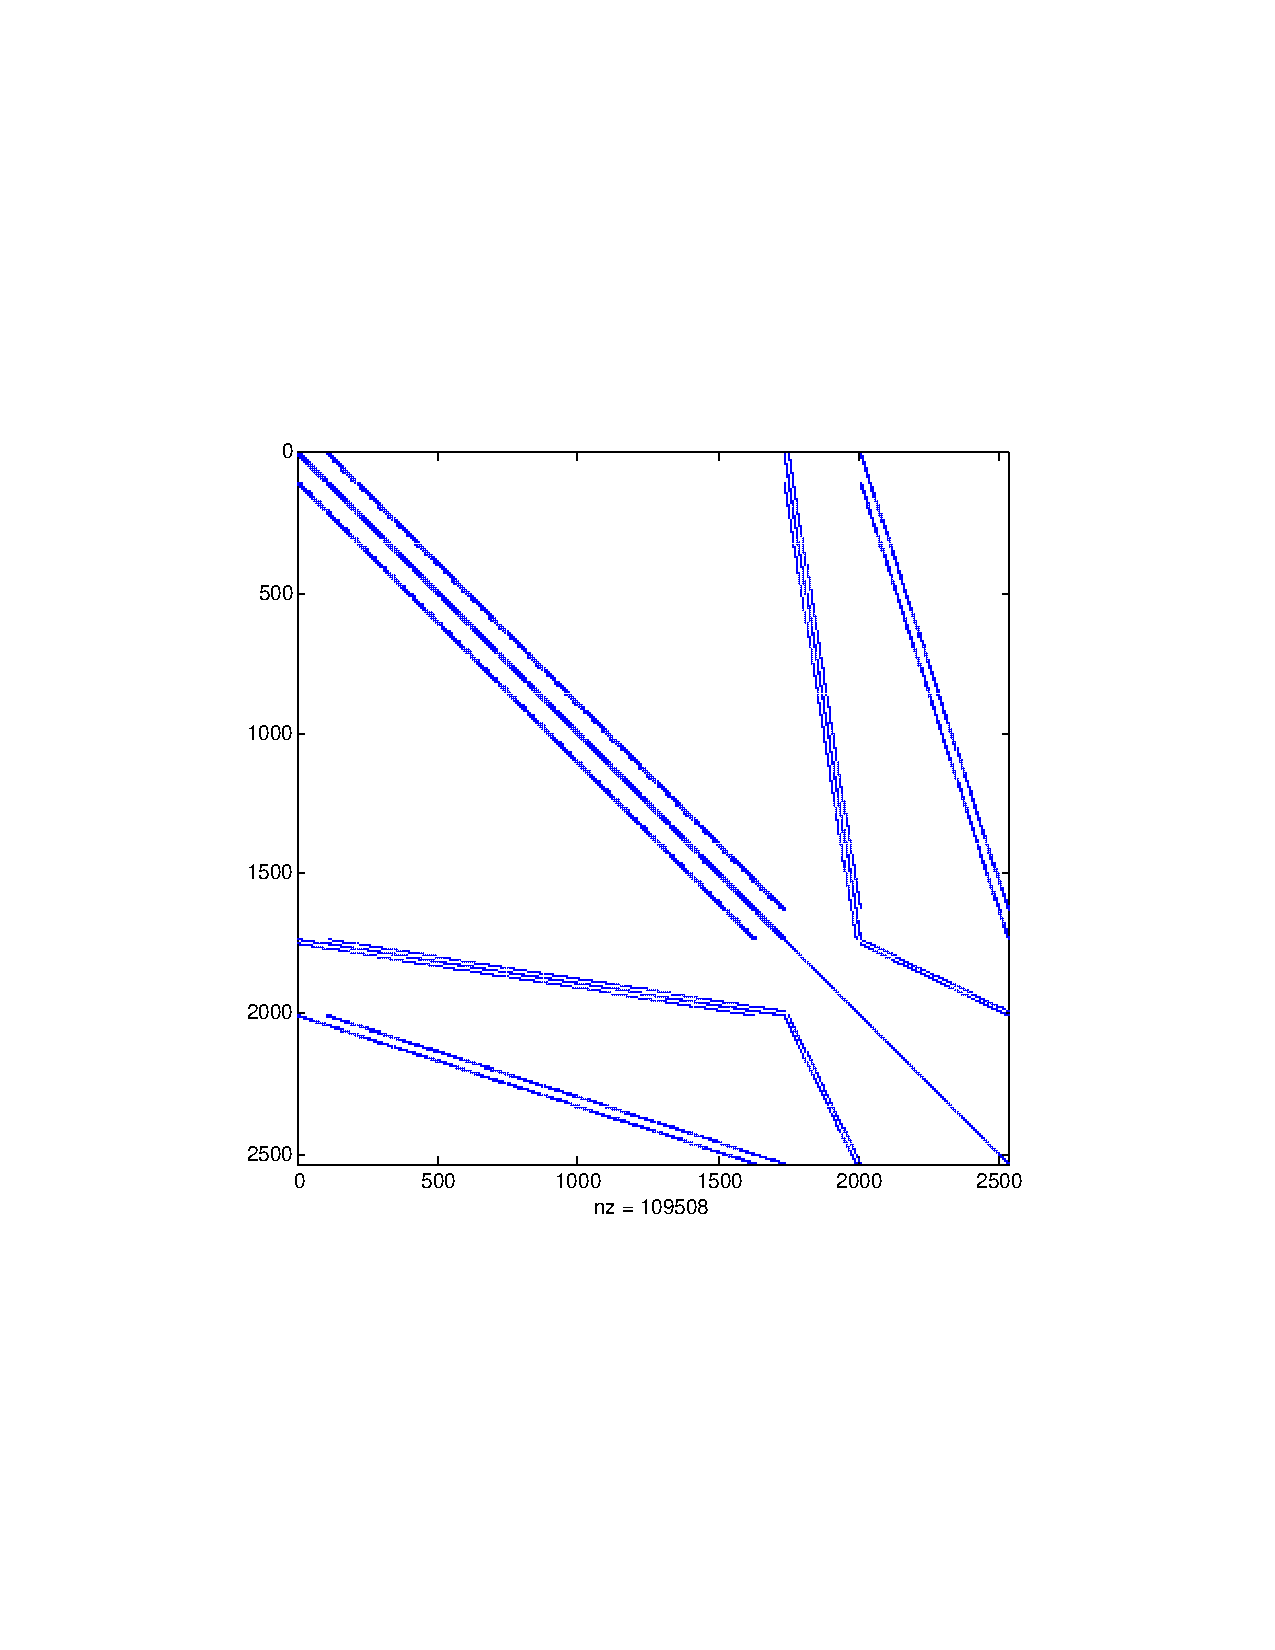
\includegraphics[trim=100 235 100 250, clip, scale=0.5]{Matrix.pdf}
	\end{center}
  \caption{Banded Stiffness Matrix as Result of Node Numbering}
	\label{fig:MatrixGraph}
\end{figure}

\subsection{Results}
In our test we take 
\begin{equation}
  u=\left( x\left( x-1 \right)y\left( y-1 \right) \right)^2 
  \label{eqn:u}
\end{equation}
be the exact solution then
\begin{equation}\begin{split}
   f= 8x^2y^2 + 24x^2(x - 1)^2 + 8x^2(y - 1)^2 + 8y^2(x - 1)^2 + 24y^2(y - 1)^2 \\
   + 8(x - 1)^2(y - 1)^2 + 32x(x - 1)*(y - 1)^2 + 32y(y - 1)(x - 1)^2 \\
   + 32xy^2(x - 1) + 32x^2y( y - 1) + 128xy(x - 1)(y - 1)
 \end{split}
   \label{eqn:f}
\end{equation}
To check the code for correctness the rate of convergence in the
$L^2,\,H^1,\text{ and } H^2$ norms were checked. Given the exact solution is $u$
and the approximate solution is $v_{h}$ then the norms are as follows
\begin{align*}
  E_{L^2}(h)=\|u-v_h\|_{L^2} &= \left(\int_{\Omega}\! (u-v_h)^2 \,d\Omega\right)^{\nicefrac{1}{2}}\\
  E_{H^1}(h)=\|u-v_h\|_{H^1} &= \left(\int_{\Omega}\! \sum_{|\alpha|\le 1}
    \left(D^{\alpha}u-D^{\alpha}v_h\right)^2 \,d\Omega\right)^{\nicefrac{1}{2}}\\
  E_{H^2}(h)=\|u-v_h\|_{H^2} &= \left(\int_{\Omega}\! \sum_{|\alpha|\le 2}
    \left(D^{\alpha}u-D^{\alpha}v_h\right)^2 \,d\Omega\right)^{\nicefrac{1}{2}}
\end{align*}
Finally, if $h_i$ is taken to be the mesh size for the current the simulation
then the rate of convergence is taken to be 
\begin{equation*}
  \dfrac{\log(|\nicefrac{E(h_{i-1})}{E(h_i)}|)}{\log(\nicefrac{h_{i-1}}{h_i})} 
\end{equation*}
For our calculations we chose a uniform grid of right isosceles triangles with
leg $h=\{\nicefrac{1}{2},\nicefrac{1}{4},\nicefrac{1}{8},\nicefrac{1}{16}\}$
and the resulting errors and observed rates of convergence can be seen in Table \ref{tab:Errors} 
\begin{table}[h]
  \begin{center}
    \caption{Table of Errors and Observed Rates of Convergence}
{\small
\begin{equation*}
  \begin{array}{|c|c|c|c|c|c|c|}
    \hline
    h & e_2 & L^2\, order & e_{H^1} & H^1\, order &e_{H^2} & H^2\, order \\[0.5em]
    \hline
    0.5 & 6.377\times 10^{-5} & NaN & 5.876\times 10^{-4} & NaN & 9.159\times 10^{-3} & NaN \\[0.5em]
    0.25 & 1.085\times 10^{-6} & 5.878 & 2.607\times 10^{-5} & 4.494 & 7.961\times 10^{-4} & 3.524 \\[0.5em]
    0.125 & 1.24\times 10^{-8} & 6.451 & 6.836\times 10^{-7} & 5.253 & 4.52\times 10^{-5} & 4.139 \\[0.5em]
    0.0625 & 1.434\times 10^{-10} & 6.434 & 1.742\times 10^{-8} & 5.294 & 2.473\times 10^{-6} & 4.192 \\[0.5em]
    \hline
  \end{array}
\end{equation*}}
\end{center}
\label{tab:Errors}
\end{table}
As can be the observed from the table the rate of convergence is seen to be
around $6$ for $L^2$, $5$ for $H^1$, and $4$ for $H^2$ which agree with the
theory.

    \section{SQGE} \label{sec:SQGETests}
    The main goal of this section is twofold. First, we show that the FE
discretization of the streamfunction formulation of the SQGE \eqref{sqge_psi_1}
with the Argyris element produces accurate numerical approximations. To this
end, we benchmark our numerical results against those in the published
literature \cite{Vallis06, Cascon, Myers}. The second goal is to show that the
numerical results follow the theoretical error estimates in
\autoref{thm:EnergyNorm} and \autoref{thm:Errors}, i.e., we compare the observed
rates of convergence to the theoretical rates of convergence developed in
\autoref{sec:SQGEErrors}.

Although the pure streamfunction formulation of the steady SQGE
\eqref{sqge_psi_1} is our main concern, we also test our Argyris FE
discretization on two simplified settings: \begin{inparaenum}[(i)] \item the
\emph{Linear Stommel} model; and \item \emph{Linear Stommel-Munk} model.
\end{inparaenum} The reason for using these two additional numerical tests is
that they are standard test problems in the geophysical fluid dynamics
literature (see, e.g., Chapter 13 in Vallis \cite{Vallis06} as well as the
reports of Myers \emph{et al.} \cite{Myers}, and Cascon \emph{et al.}
\cite{Cascon}). This allows us to benchmark our numerical results against
those in the published literature. Since both the Linear Stommel and the
Linear Stommel-Munk models lack the nonlinearity present in the SQGE
\eqref{sqge_psi_1}, the represent good stepping stones to verifying our FE
discretization.

The \emph{Linear Stommel-Munk} model (see p. 587 in \cite{Vallis06} and problem
2 in \cite{Cascon}) is given by
\begin{equation}
  \epsilon_s \Delta \psi - \epsilon_m \Delta^2 \psi + \frac{\partial \psi}{\partial x} = f,
  \label{eqn:Stommel-Munk}
\end{equation}
where $\epsilon_s \text{ and } \epsilon_m$ are the Stommel Number and Munk
Scale, respectively. The Stommel Number and Munk Scale are given by (Equation 10
in \cite{Myers})
\begin{equation*}
  \epsilon_m = \frac{A}{\beta L^3} \qquad \epsilon_s = \frac{\gamma}{\beta L}
\end{equation*}
where $A,\, \beta,\, L, \text{ and } \gamma$ are the eddy visosity, the
$\beta$-plane effect, characteristic length scale, and the bottom friction decay
rate, respectively. The model is supplemented with appropriate boundary
conditions, which will be described for each of the subsequent numerical tests.

We note that the Linear Stommel-Munk model \eqref{eqn:Stommel-Munk} is similar
in form to the SQGE \eqref{sqge_psi_1}. Indeed, both models contain the
biharmonic operator $\Delta^2 \psi$, the rotation term $\dfrac{\partial
\psi}{\partial x}$, and the forcing term $F$. The two main differences between
the two models are the following: First, the SQGE are nonlinear, since they
contain the Jacobian term $J(\psi,q)$; the Stommel-Munk model is linear, since
it doesn't contain the Jacobian term. The second difference is that the Linear
Stommel-Munk model contains a Laplacian term $\Delta \psi$, whereas the SQGE
does not.

We also note that the two models use different parameters: the Reynolds number
$Re$ and the Rossby number $Ro$ in \eqref{sqge_psi_1} and the Stommel number
$\epsilon_s$ and the Munk scale $\epsilon_m$ in the Linear Stommel-Munk model.
These two sets of parameters, however, are related by the following relations:
\begin{align}
  \epsilon_m &= Ro\, Re^{-1} \label{eqn:MunkScale}\\
  \epsilon_s &= Ro \frac{\gamma\, L}{U} \label{eqn:StommelNumber}\\
\end{align}
%\textcolor{red}{If $\gamma \sim T$ then $\epsilon = Ro$. However, I am unsure this is a valid
%assumption and so I am having trouble relating the Stommel Number to Reynolds and Rosby.}

The second simplified model used in our numerical investigation is the
\emph{Linear Stommel} model (Equation 14.22 in \cite{Vallis06} and Equation 11
in \cite{Myers})
\begin{equation}
  \epsilon_s \Delta \psi + \frac{\partial \psi}{\partial x} = f.
  \label{eqn:Stommel}
\end{equation}
We note that the Linear Stommel Model \eqref{eqn:Stommel} is just the Linear
Stommel-Munk model \eqref{eqn:Stommel-Munk} in which the biharmonic term is
dropped (i.e. $\epsilon_m=0$).

The rest of the subsection is organized as follows: In \autoref{sse:LSM} we
present results for the Linear Stommel model \eqref{eqn:Stommel}. In
\autoref{sse:SMM} we present results for the Linear Stommel-Munk model
\eqref{eqn:Stommel-Munk}. Finally, in \autoref{sse:SQGE} we present results for
the nonlinear SQGE \eqref{sqge_psi_1}.

\subsection{Linear Stommel Model} \label{sse:LSM} This subsection presents the
results for the FE discretization of the Linear Stommel model
\eqref{eqn:Stommel} by using the Argyris element. The computational domain is
$\Omega = [0,1]\times [0,1]$. For completeness, we present results for two
numerical tests. The first test, denoted by Test 1, corresponds to the exact
solution used by Vallis (Equation 14.38 in \cite{Vallis06}), while the second
test, denoted by Test 2, corresponds to the exact solution used by Myers
\emph{et al.} (Equations 15 and 16 in \cite{Myers}).

\tbf{Test 1a:} In this test, we choose the same setting as that used by Vallis
(Equation 14.38 in \cite{Vallis06}).  In particular, the forcing term and the
non-homogeneous Dirichlet boundary conditions are chosen to match those given by
the exact solution
\begin{equation}
  \psi(x,y) = (1-x-e^{-\nicefrac{x}{\epsilon_s}}) \sin \pi y
  \label{eqn:MyerExact}
\end{equation}
We choose the same Stommel number as that used by Vallis, i.e.
$\epsilon_s=0.04$. The exact solution \eqref{eqn:MyerExact} considered by Vallis
satisfies $\psi \to 0$ as $x \to 0$, but does not vanish at $x=1$. In our
numerical tests, we used a standard lifting procedure to treat these
non-homogeneous boundary conditions, i.e. for a problem of the form
\begin{align*}
  L \psi&=f \text{ on } \Omega\\
  \psi &=g \text{ on } \partial \Omega,
\end{align*}
we reformulate it to be
\begin{align*}
  L\tilde{\psi} &= \tilde{f} \text{ on } \Omega \\
  \tilde{\psi} &= 0 \text{ on } \partial \Omega
\end{align*}
where $L\tilde{\psi} = Lu - LS = f - g = \tilde{f}$ and the solution $\psi$ from
the original problem can then be found by $\psi(x,y) =\tilde{\psi}+S$. The
function $S(x,y)$ is assumed to have the form
\begin{equation*}
  S(x,y) = A(y) (1-x) + B(y) x
\end{equation*}
and satisfies the boundary conditions given by \eqref{eqn:MyersExact}. After
some simple algebra we see that
\begin{equation*}
  S(x,y) = -x e^{-x/\epsilon_s}\pi \sin(\pi y).
\end{equation*}
The function $\tilde{f}$ can be determined by applying the operator $L$
corresponding to the \emph{Linear Stommel} problem to $u - S$

Applying the finite element method to the \emph{Linear Stommel} problem with the
new modified $\tilde{f}$, corresponding to the exact solution given by Vallis,
and homogeneous boundary conditions using Argyris Finite Elements we get a
solution that matches the solution presented by Vallis, as can be seen in
\autoref{fig:StommelVallis}. Additionally, the table of errors
\autoref{tab:StommelErrorsVallis} shows the order of convergence appears to be
approaching the expected rates for $L^2, H^1, \text{ and } H^2$ norms.
\autoref{fig:StommelVallis} presents the streamlines of the approximate solution
obtained by using the Argyris Finite Element on a mesh with $h=\frac{1}{32}$ and
$9670$ DoFs. Comparing \autoref{fig:StommelVallis} with Figure $14.5$ in
\cite{Vallis06}, we notice that our approximation is close to his. Since the
exact solution is available, we can compute the errors in various norms.
\autoref{tab:StommelErrorsVallis} presents the errors $e_0,\, e_1, \text{ and }
e_2$ (i.e., the $L^2,\, H^1, \text{ and } H^2$ errors, respectively) for various
values of the mesh sizes, $h$ (the DoFs are also included).

\begin{table}%[H]
\begin{center}
%{\footnotesize
\begin{tabular}{|c|c|c|c|c|c|c|c|}%c|c|}
  \hline
  $h$ & $DoFs$ & $e_0$ & $L_2$ order & $e_1$ & $H^1$ order & $e_2$ & $H^2$ order \\[0.2em] % & $e_{\infty}$ & $L_{\infty}$ order \\
  \hline
  $\nicefrac{1}{2}$ & $70$ & $0.1148$ & $-$ & $1.81$ & $-$ & $83.67$ & $-$ \\[0.2em] % & $0.00681$ & $-$ \\
  $\nicefrac{1}{4}$ & $206$ & $0.01018$ & $3.495$ & $0.312$ & $2.537$ & $25.48$ & $1.716$ \\[0.2em] % & $0.007801$ & $-0.1961$ \\
  $\nicefrac{1}{8}$ & $694$ & $0.0004461$ & $4.512$ & $0.02585$ & $3.593$ & $3.902$ & $2.707$ \\[0.2em] % & $0.0004681$ & $4.059$ \\
  $\nicefrac{1}{16}$ & $2534$ & $1.09\times 19^{-5}$ & $5.355$ & $0.001215$ & $4.412$ & $0.3494$ & $3.481$ \\[0.2em] % & $1.732\times 19^{-5}$ & $4.756$ \\
  $\nicefrac{1}{32}$ & $9670$ & $1.972\times 19^{-7}$ & $5.788$ & $4.349\times 19^{-5}$ & $4.804$ & $0.02335$ & $3.903$ \\[0.2em] % & $5.396\times 19^{-7}$ & $5.005$ \\
  \hline
\end{tabular}
%}
\end{center}
\caption{Errors and Rate of Convergence for the Linear Stommel Model \eqref{eqn:Stommel}, Test 1 \cite{Vallis06}}
\label{tab:StommelErrorsVallis}
\end{table}

\begin{figure}%[H]
  \begin{center}
    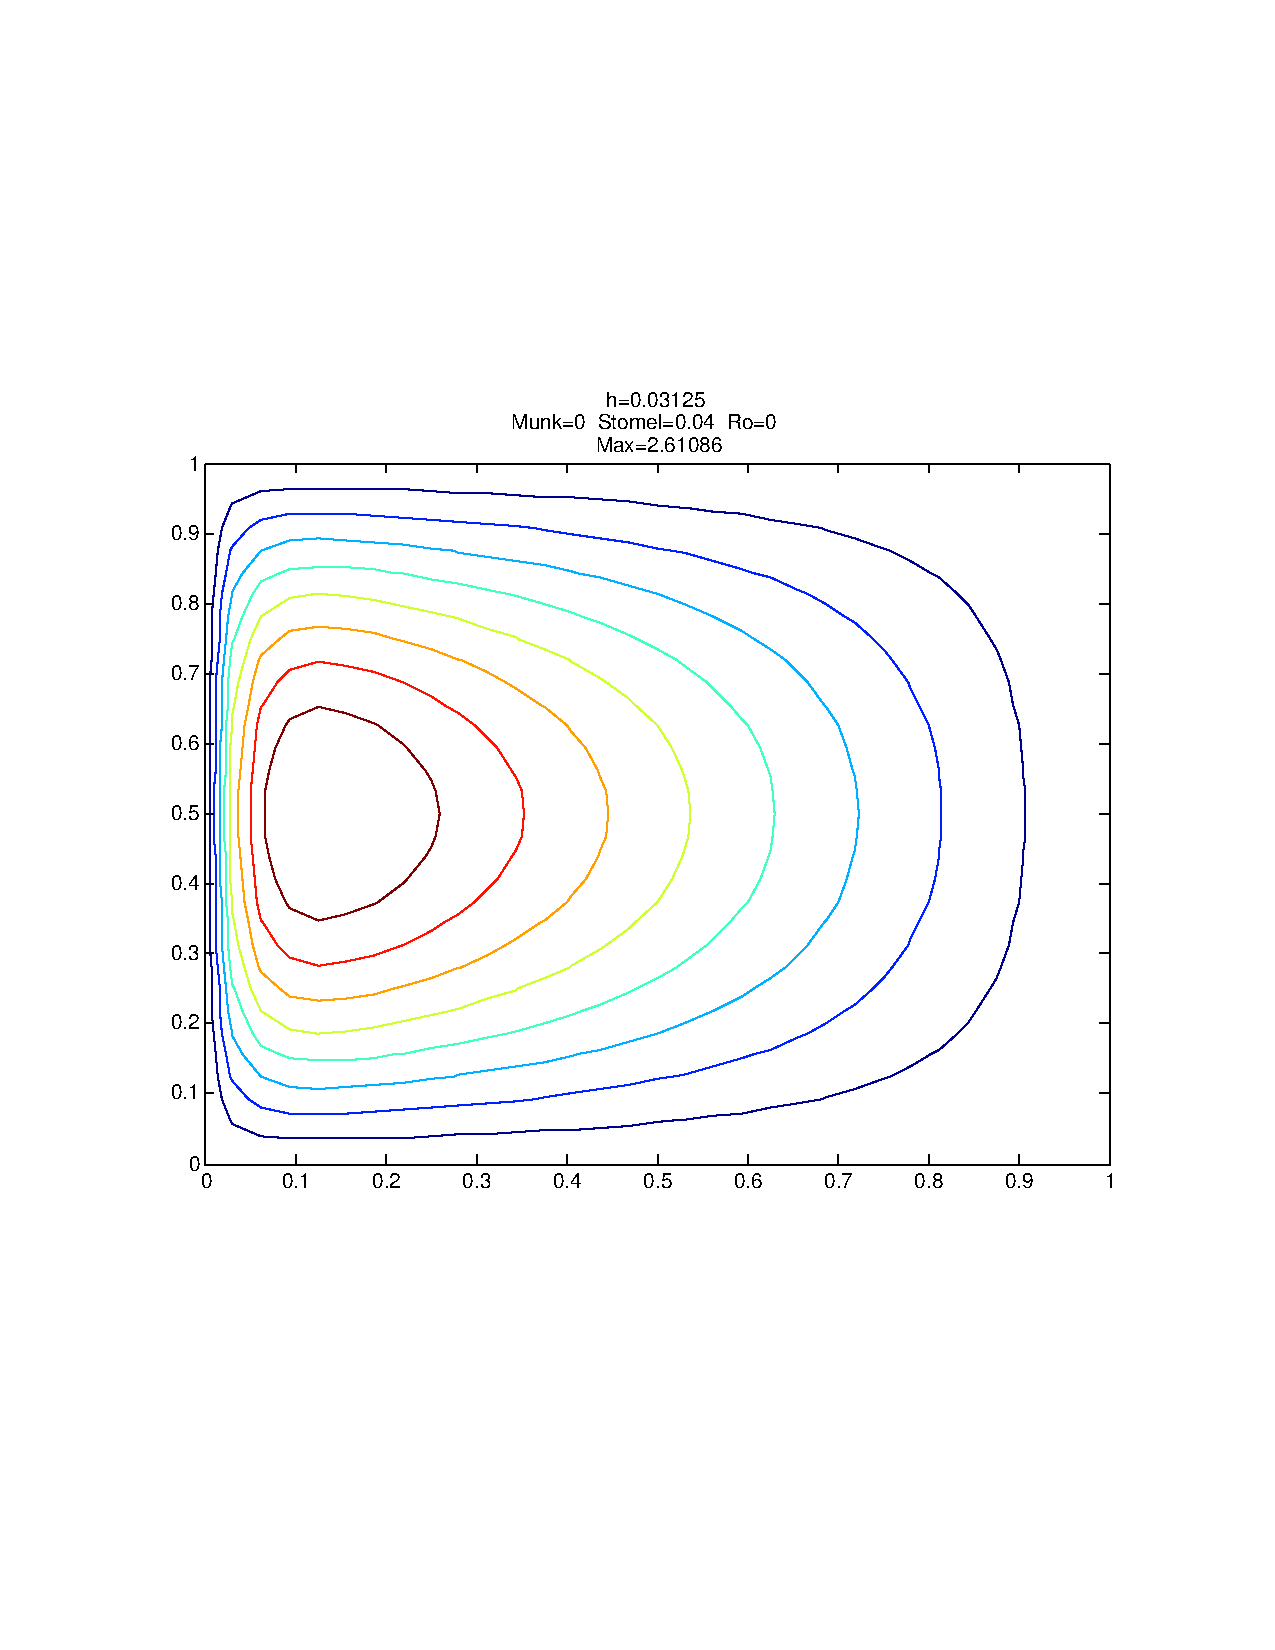
\includegraphics[trim=0 200 20 220, clip=true, scale=0.5]{LinearStommelVallis.pdf}
    \caption{Linear Stommel Model \eqref{eqn:Stommel}, Test 1a \cite{Vallis06}: Streamlines of the approximation,
    $\psi^h$, $h=\frac{1}{32}$, and $9670$ DoFs.}
    \label{fig:StommelVallis}
  \end{center}
\end{figure}
We note that the errors in \autoref{tab:StommelErrorsVallis} follow the
theoretical rates of convergence predicted by the estimates \eqref{eqn:H2Error}
- \eqref{eqn:L2Error} in \autoref{thm:Errors}. The orders of convergence in
\autoref{tab:StommelErrorsVallis} are close to the theoretical ones for the fine
meshes, but not as close for the coarse meshes. We think that the inaccuracies
on the coarse meshes are due to their inability to capture the thin boundary
layer on the left-hand side (i.e., at $x=0$). The finer the mesh gets, the
better this boundary layer is captured and the better the numerical accuracy
becomes.

\tbf{Test 1b:}
In the Second part of Test 1, we verify the hypothesis above, that is, whether
the degrading accuracy of the approximation is indeed due to the thin western
boundary layer. To this end, we change the Stommel number in Test 1a to be
$\epsilon_s=1$, which will result in a much thicker western boundary layer. We
then run the same numerical test as before, but with the new Stommel number. As
can be seen in \autoref{tab:StommelErrorsVallise1}, the rates of convergence are
the expected theoretical orders of convergence. This shows that the reason for
the inaccuracies in \autoref{tab:StommelErrorsVallis} were indeed due to the
thin western boundary layer.

\begin{table}%[H]
\begin{center}
%{\scriptsize
\begin{tabular}{|c|c|c|c|c|c|c|c|}%c|c|}
  \hline
  $h$ & $DoFs$ & $e_0$ & $L_2$ order & $e_1$ & $H^1$ order & $e_2$ & $H^2$ order \\[0.2em] % & $e_{\infty}$ & $L_{\infty}$ order \\
  \hline
  $\nicefrac{1}{2}$ & $70$ & $1.689\times 10^{-5}$ & $-$ & $0.0003434$ & $-$ & $0.008721$ & $-$ \\[0.2em] % & $4.306\times 10^{-6}$ & $-$ \\
  $\nicefrac{1}{4}$ & $206$ & $3.722\times 10^{-7}$ & $5.504$ & $1.341\times 10^{-5}$ & $4.678$ & $0.0005616$ & $3.957$ \\[0.2em] % & $5.542\times 10^{-7}$ & $2.958$ \\
  $\nicefrac{1}{8}$ & $694$ & $4.891\times 10^{-9}$ & $6.25$ & $3.757\times 10^{-7}$ & $5.158$ & $3.25\times 10^{-5}$ & $4.111$ \\[0.2em] % & $9.043\times 10^{-9}$ & $5.937$ \\
  $\nicefrac{1}{16}$ & $2534$ & $7.079\times 10^{-11}$ & $6.111$ & $1.117\times 10^{-8}$ & $5.071$ & $1.964\times 10^{-6}$ & $4.049$ \\[0.2em] % & $1.355\times 10^{-10}$ & $6.06$ \\
  $\nicefrac{1}{32}$ & $9670$ & $1.08\times 10^{-12}$ & $6.035$ & $3.437\times 10^{-10}$ & $5.023$ & $1.213\times 10^{-7}$ & $4.018$ \\[0.2em] % & $2.169\times 10^{-12}$ & $5.965$ \\
  \hline
\end{tabular}
%}
\end{center}
\caption{Errors and Rate of Convergence for the Linear Stommel Model \eqref{eqn:Stommel}, Test 1b \cite{Vallis06}}
\label{tab:StommelErrorsVallise1}
\end{table}

\begin{figure}%[H]
  \begin{center}
    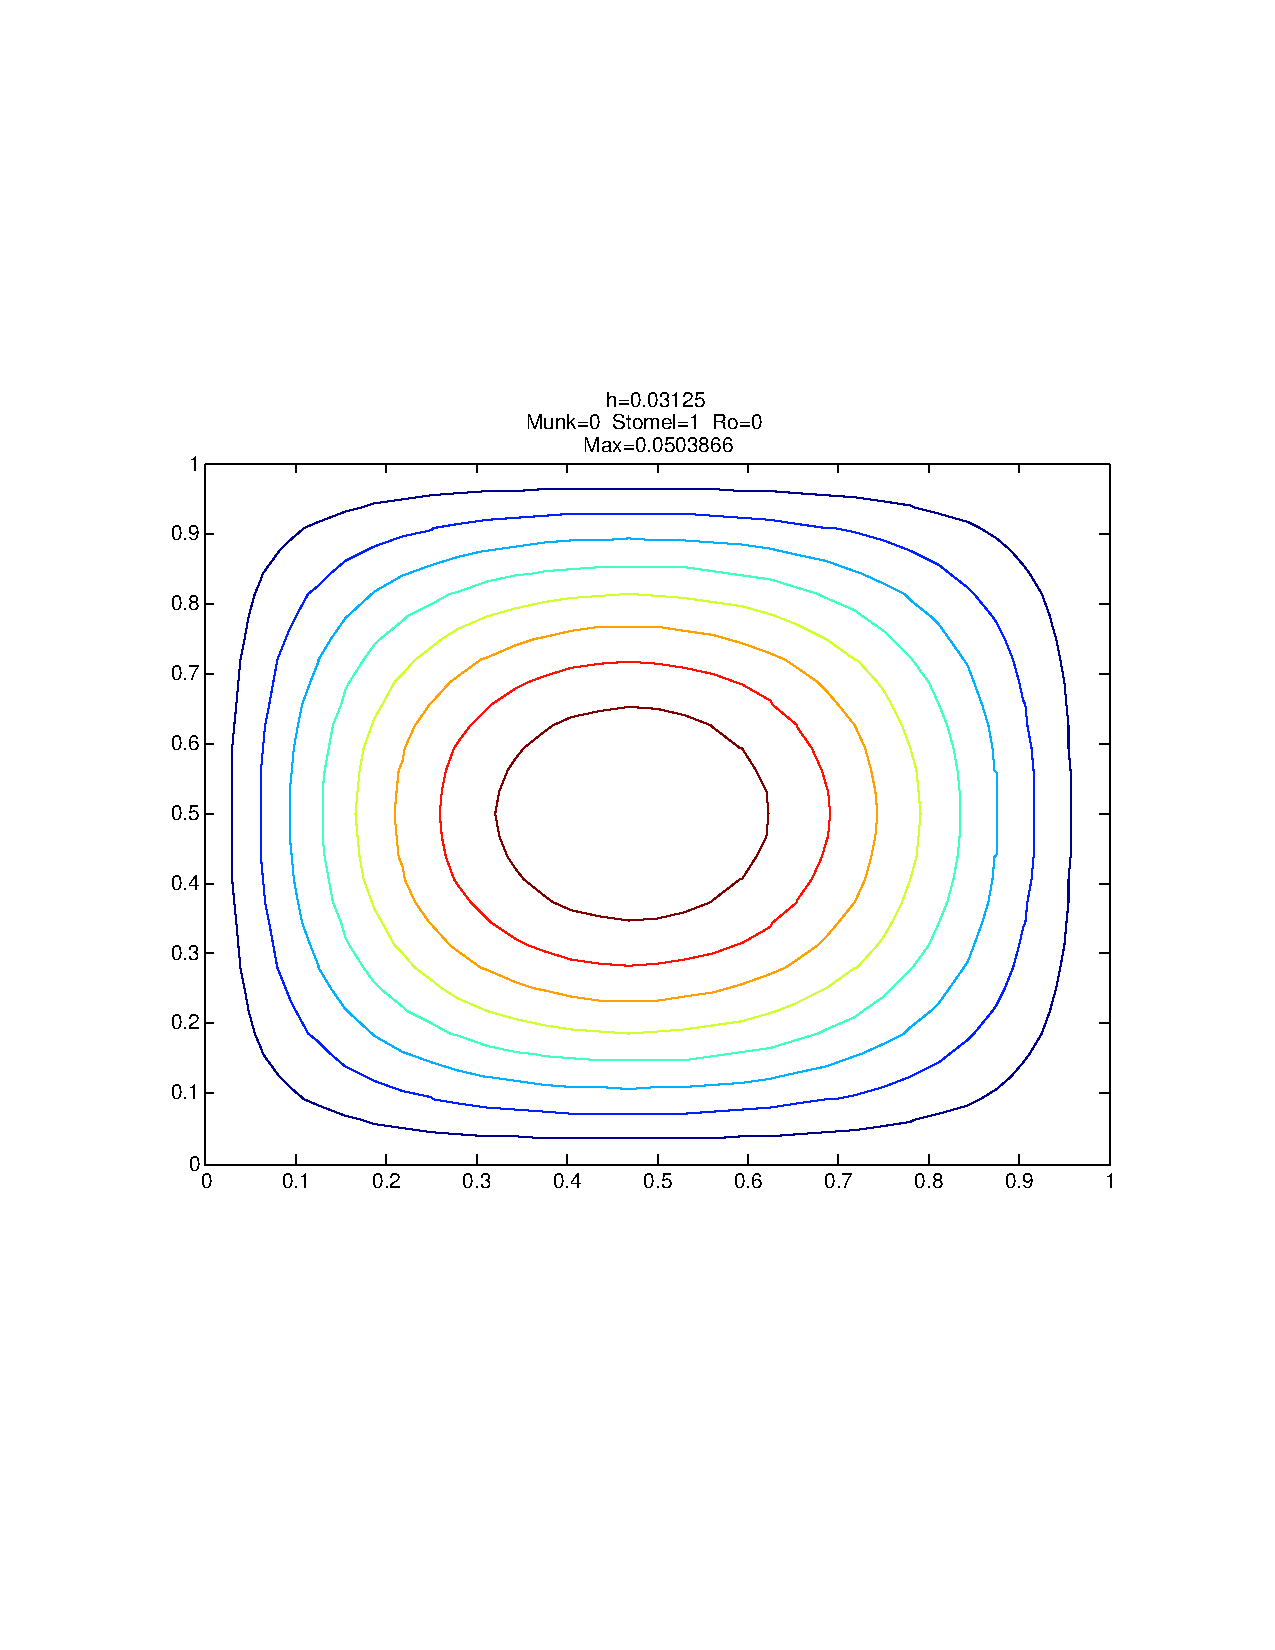
\includegraphics[trim=0 200 20 220, clip=true, scale=0.5]{StommelVallise1.pdf}
    \caption{Linear Stommel Model \eqref{eqn:Stommel}, Test 1b \cite{Vallis06}: Streamlines of the approximation,
    $\psi^h$, $h=\frac{1}{32}$, and $9670$ DoFs with $\epsilon_s=1$.}
    \label{fig:StommelVallise1}
  \end{center}
\end{figure}

\tbf{Test 2:}
For our second test we use the exact solution given by Myers (Equations 15 and
16 in \cite{Myers}), i.e.
{\footnotesize
\begin{equation}
  \psi(x,y) =\frac{\sin(\pi y)}{\pi(1+4\pi^2\epsilon_s^2)}\left\{2\pi\epsilon_s\sin(\pi x)+cos(\pi x)+\frac{1}{e^{R_1}-e^{R_2}}\left[(1+e^{R_2})e^{R_1x}-(1+e^{R_1})e^{R_2x}\right]\right\},
  \label{eqn:MyersExact}
\end{equation}
}
where $R_1\text{ and } R_2$ are the positive and negative roots, respectively,
of
\begin{equation*}
  R = \frac{-1\pm\sqrt{1+4\pi^2 \epsilon_s^2}}{2\epsilon_s}.
\end{equation*}
The forcing term and the homogeneous Dirichlet boundary conditions are chosen to
match those given by the exact solution \eqref{eqn:MyersExact}. We choose the
same Stommel number as that used by Myers, i.e. $\epsilon_s=0.05$.

\autoref{fig:StommelMyers} presents the streamlines of the approximate solution
obtained by using the Argyris Finite Element on a mesh with $h=\frac{1}{32}$ and
$9670$ DoFs. Comparing \autoref{fig:StommelMyers} with Figure $2$ in
\cite{Myers}, we notice that our approximation is close to that in \cite{Myers}.
Since the exact solution is available, we can compute the errors in various
norms. \autoref{tab:StommelErrorsMyers} presents the errors $e_0,\, e_1, \text{
and } e_2$ (i.e., the $L^2,\, H^1, \text{ and } H^2$ errors, respectively) for
various values of the mesh sizes, $h$.

\begin{table}%[H]
\begin{center}
%{\footnotesize
\begin{tabular}{|c|c|c|c|c|c|c|c|}%c|c|}
  \hline
  $h$ & $DoFs$ & $e_0$ & $L_2$ order & $e_1$ & $H^1$ order & $e_2$ & $H^2$ order \\[0.2em] % & $e_{\infty}$ & $L_{\infty}$ order \\
  \hline
  $\nicefrac{1}{2}$ & $70$ & $0.005645$ & $-$ & $0.1451$ & $-$ & $6.602$ & $-$ \\[0.2em] % & $0.0008815$ & $-$ \\
  $\nicefrac{1}{4}$ & $206$ & $0.0004276$ & $3.723$ & $0.02081$ & $2.801$ & $1.632$ & $2.016$ \\[0.2em] % & $0.0003139$ & $1.49$ \\
  $\nicefrac{1}{8}$ & $694$ & $1.46\times 10^{-5}$ & $4.872$ & $0.001408$ & $3.886$ & $0.2066$ & $2.982$ \\[0.2em] % & $2.15\times 10^{-5}$ & $3.868$ \\
  $\nicefrac{1}{16}$ & $2534$ & $2.954\times 10^{-7}$ & $5.627$ & $5.829\times 10^{-5}$ & $4.594$ & $0.0165$ & $3.646$ \\[0.2em] % & $7.097\times 10^{-7}$ & $4.921$ \\
  $\nicefrac{1}{32}$ & $9670$ & $4.968\times 10^{-9}$ & $5.894$ & $1.998\times 10^{-6}$ & $4.867$ & $0.001069$ & $3.948$ \\[0.2em] % & $2.054\times 10^{-8}$ & $5.111$ \\
  \hline
\end{tabular}
%}
\end{center}
\caption{Errors and Rate of Convergence for the Linear Stommel Model \eqref{eqn:Stommel}, Test 2 \cite{Myers}}
\label{tab:StommelErrorsMyers}
\end{table}

\begin{figure}%[H]
  \begin{center}
    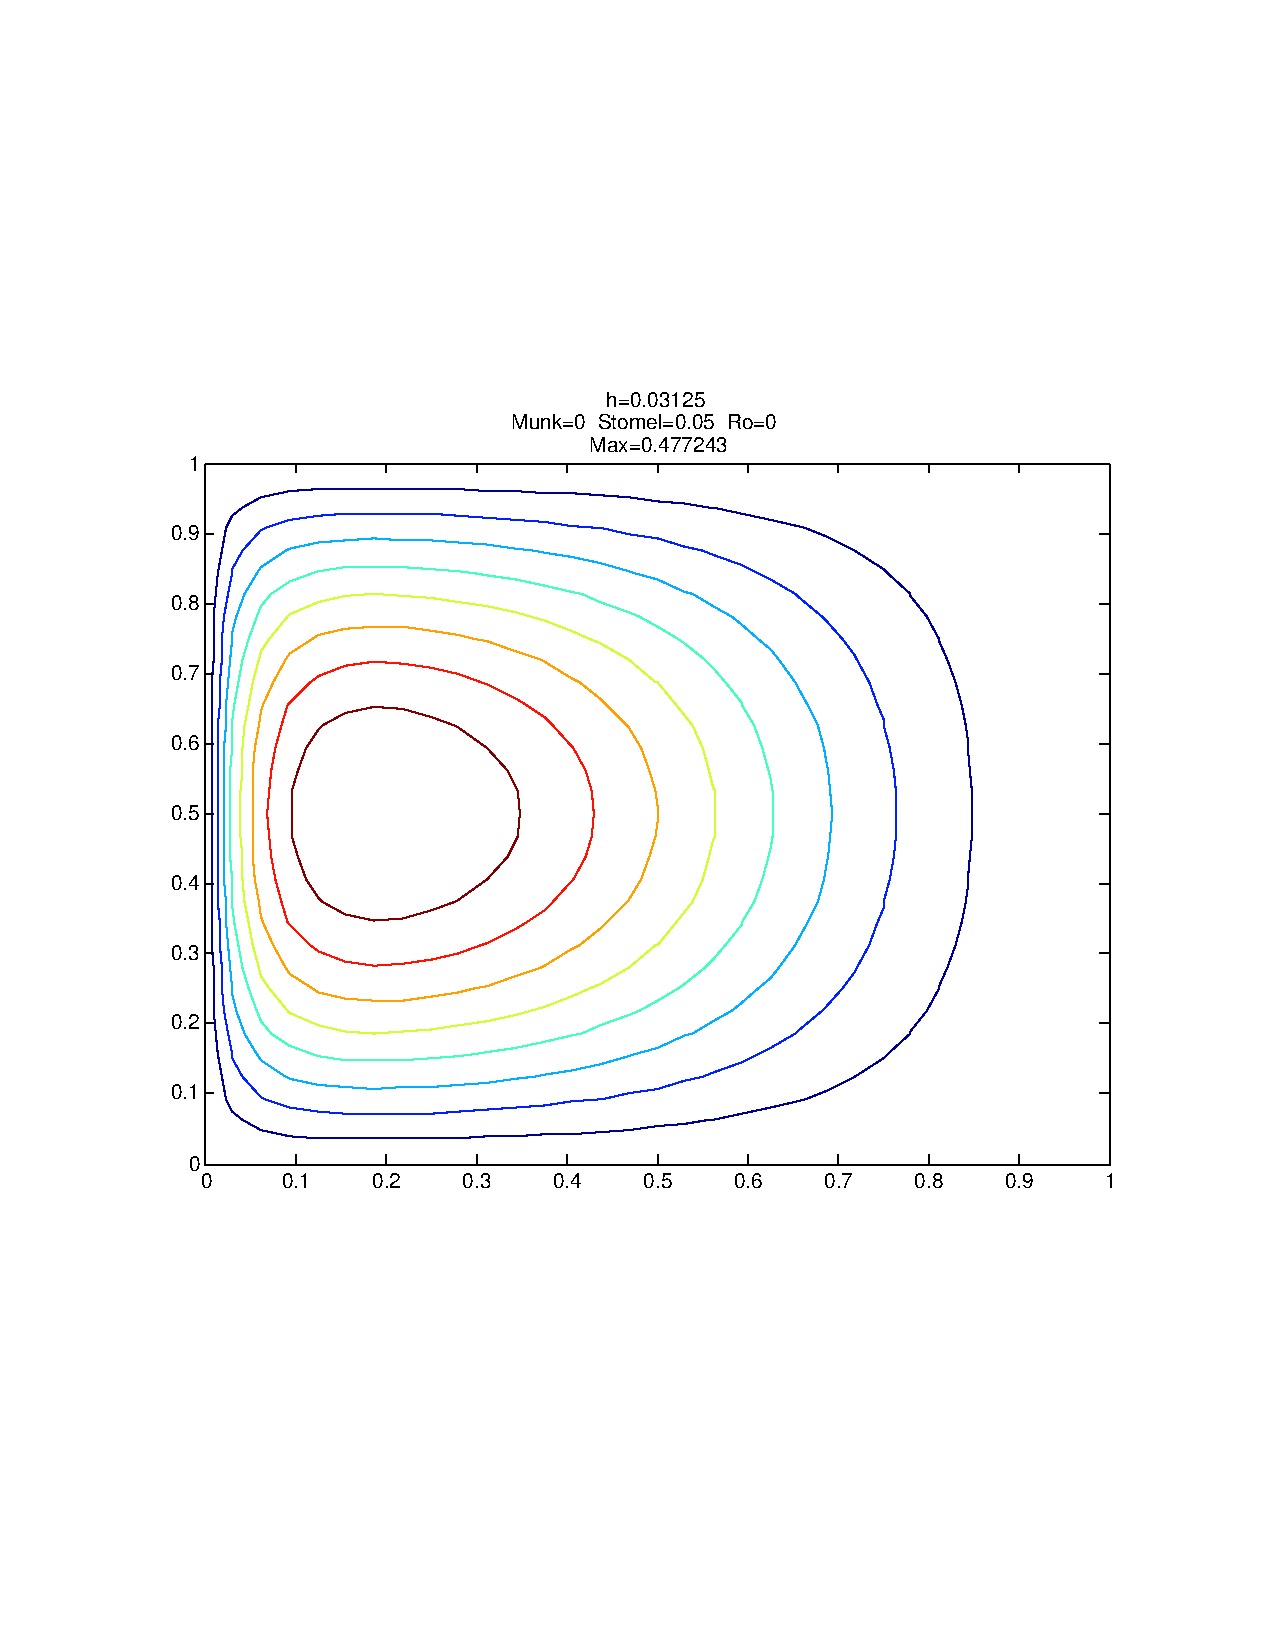
\includegraphics[trim=0 200 20 220, clip=true, scale=0.5]{LinearStommelMyers.pdf}
    \caption{Linear Stommel Model \eqref{eqn:Stommel}, Test 2 \cite{Myers}: Streamlines of the approximation,
    $\psi^h$, $h=\frac{1}{32}$, and $9670$ DoFs.}
    \label{fig:StommelMyers}
  \end{center}
\end{figure}

We note that the errors in \autoref{tab:StommelErrorsMyers} follow the
theoretical rates of convergence predicted by the estimates \eqref{eqn:H2Error}
- \eqref{eqn:L2Error} in \autoref{thm:Errors}. Again, we see that the orders of
convergence in \autoref{tab:StommelErrorsMyers} are close to the theoretical
ones for the fine meshes, but not as close for the coarse meshes. We attribute
this to the inaccuracies at the thin boundary layer on the left-hand side (i.e.,
at $x=0$). The finer the mesh gets, the better this boundary layer is captured
and the better the numerical accuracy becomes.

\subsection{Linear Stommel-Munk Model}\label{sse:SMM}
This subsection presents results for the FE discretization of the Linear
Stommel-Munk model \eqref{eqn:Stommel-Munk} by using the Argyris element. Our
computational setting is the same as taht used by Cascon \emph{et al.}
\cite{Cascon}: The computational domain is $\Omega = [0,3]\times[0,1]$, the Munk
scale is $\epsilon_m=6\times 10^{-5}$, the Stommel number is $\epsilon_s=0.05$,
and the boundary conditions are
\begin{equation} \label{eqn:SMProb}
  \psi = \frac{\partial \psi}{\partial \mathbf{n}}=0 \quad \text{ on } \partial\Omega
\end{equation}
For completeness, we present results for two numerical tests, denoted by Test 3
and Test 4, both corresponding to Test 1 and Test 2 in \cite{Cascon},
respectively.

\tbf{Test 3:}
For our third test we use the exact solution given by Test 1 in \cite{Cascon},
i.e.
\begin{equation}
  \psi(x,y) = \sin^2 \frac{\pi x}{3} \sin^2 \pi y.
  \label{eqn:CasconExact1}
\end{equation}
The forcing term is chosen to match that given by the exact solution
\eqref{eqn:CasconExact1}.

For this third test we take $F$ corresponding to applying the linear operator
$L$ associated with the \emph{Linear Stommel-Munk} model to the exact solution
\eqref{eqn:CasconExact1}.

\autoref{fig:StommelMunkSin} presents the streamlines of the approximate
solution obtained by using the Argyris Finite Element on a mesh with
$h=\frac{1}{32}$ and $28550$ DoFs. Comparing \autoref{fig:StommelMunkSin} with
Figure $7$ in \cite{Myers}, we notice that our approximation is close to that in
\cite{Myers}. Since the exact solution is available, we can compute the errors
in various norms. \autoref{tab:SMsinErrors} presents the errors $e_0,\, e_1,
\text{ and } e_2$ (i.e., the $L^2,\, H^1, \text{ and } H^2$ errors,
respectively) for various values of the mesh sizes, $h$.

\begin{table}%[H]
\begin{center}
%{\scriptsize
\begin{tabular}{|c|c|c|c|c|c|c|c|}%c|c|}
  \hline
  $h$ & $DoFs$ & $e_0$ & $L_2$ order & $e_1$ & $H^1$ order & $e_2$ & $H^2$ order \\[0.2em] % & $e_{\infty}$ & $L_{\infty}$ order \\
  \hline
  $\nicefrac{1}{2}$ & $170$ & $0.00299$ & $-$ & $0.04084$ & $-$ & $0.7624$ & $-$ \\[0.2em] % & $0.003423$ & $-$ \\
  $\nicefrac{1}{4}$ & $550$ & $3.217\times 10^{-5}$ & $6.539$ & $0.001031$ & $5.308$ & $0.04078$ & $4.225$ \\[0.2em] % & $1.885\times 10^{-5}$ & $7.505$ \\
  $\nicefrac{1}{8}$ & $1958$ & $3.437\times 10^{-7}$ & $6.548$ & $2.491\times 10^{-5}$ & $5.371$ & $0.002253$ & $4.178$ \\[0.2em] % & $2.371\times 10^{-7}$ & $6.313$ \\
  $\nicefrac{1}{16}$ & $7366$ & $4.571\times 10^{-9}$ & $6.232$ & $7.026\times 10^{-7}$ & $5.148$ & $0.0001344$ & $4.067$ \\[0.2em] % & $4.296\times 10^{-9}$ & $5.786$ \\
  $\nicefrac{1}{32}$ & $28550$ & $6.704\times 10^{-11}$ & $6.091$ & $2.113\times 10^{-8}$ & $5.056$ & $8.26\times 10^{-6}$ & $4.024$ \\[0.2em] % & $6.86\times 10^{-11}$ & $5.969$ \\
 \hline
\end{tabular}
%}
\end{center}
\caption{Errors and Rate of Convergence for the Linear Stommel-Munk Model \eqref{eqn:SMProb}, Test 3 \cite{Cascon}}
\label{tab:SMsinErrors}
\end{table}

\begin{figure}%[H]
  \begin{center}
    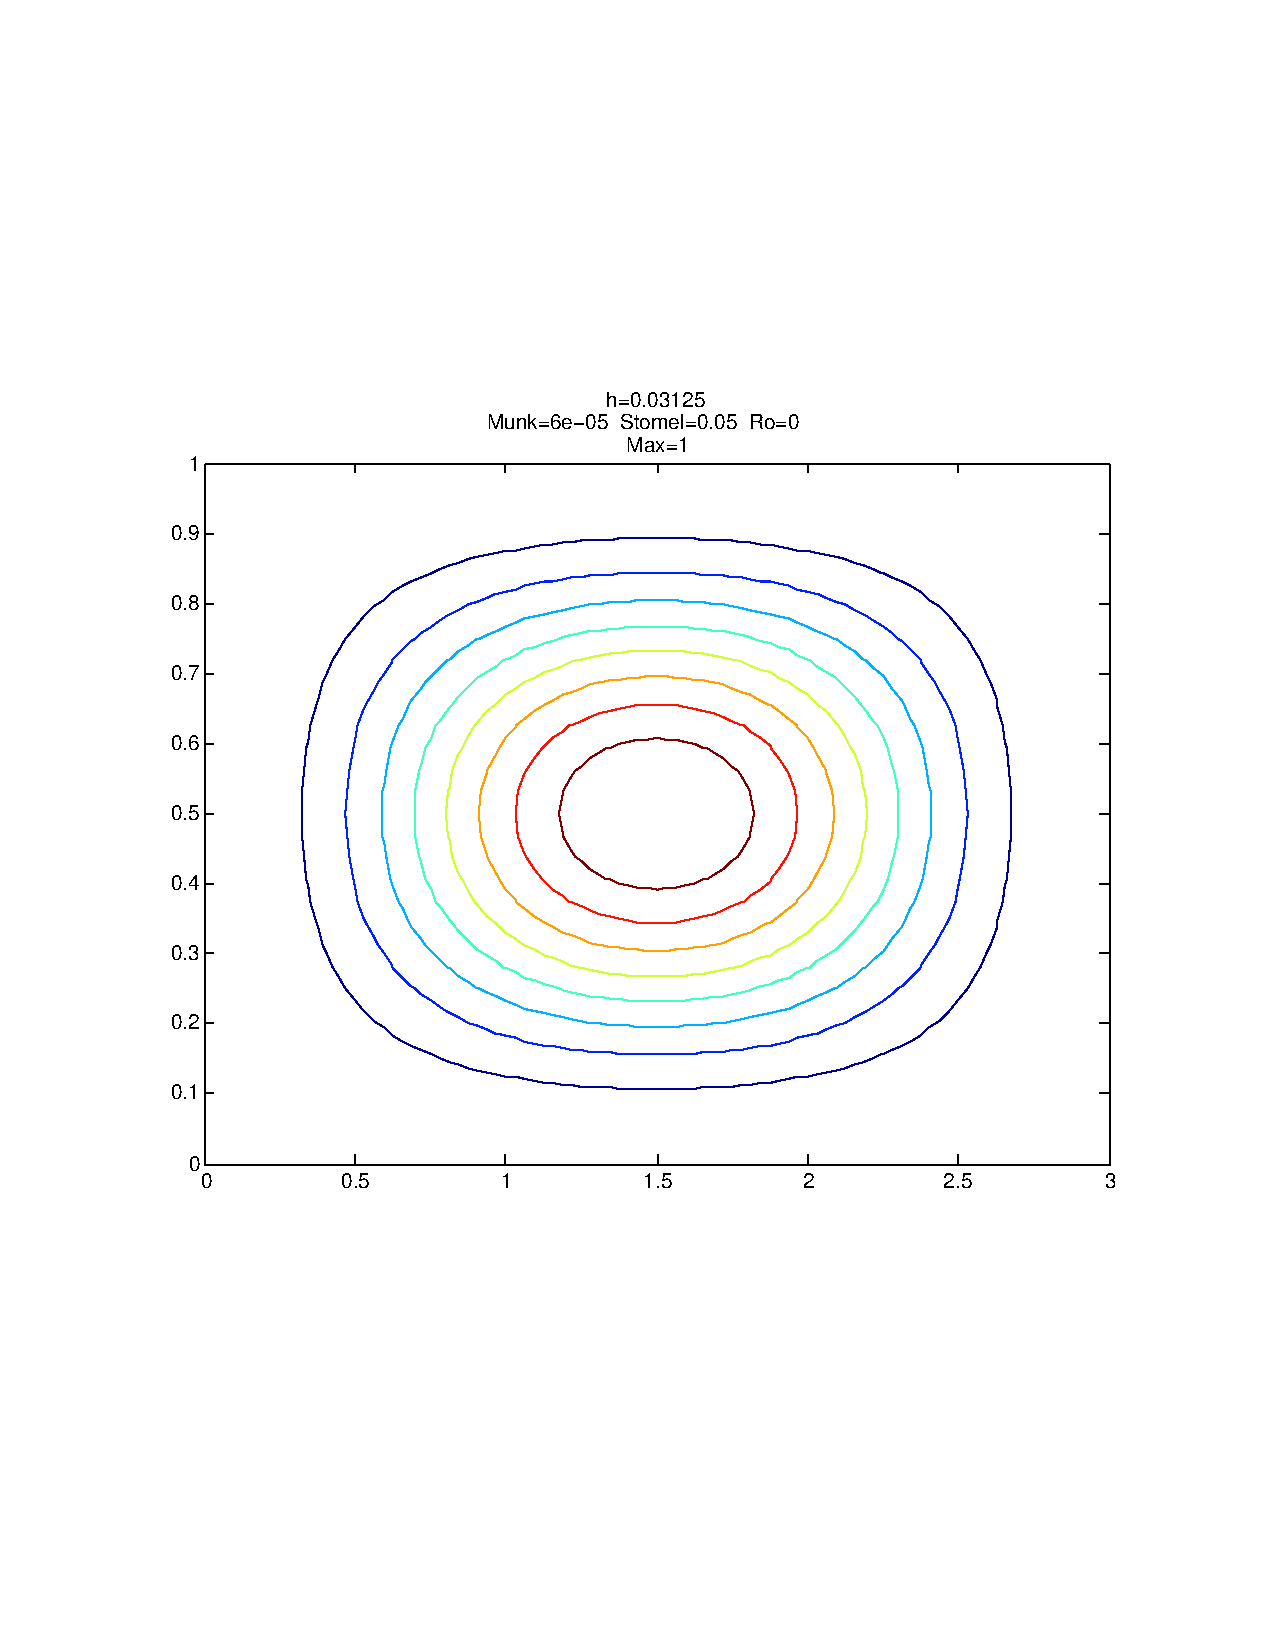
\includegraphics[trim=0 200 20 220, clip=true, scale=0.5]{StommelMunk1.pdf}
    \caption{Linear Stommel-Munk Model \eqref{eqn:SMProb}, Test 3 \cite{Cascon}: Streamlines of the approximation,
    $\psi^h$, on a mesh size, $h=\frac{1}{32}$, and $28550$ DoFs.}
    \label{fig:StommelMunkSin}
  \end{center}
\end{figure}

We note that the errors in \autoref{tab:SMsinErrors} follow the theoretical
rates of convergence predicted by the estimates \eqref{eqn:H2Error} -
\eqref{eqn:L2Error} in \autoref{thm:Errors}.  This time, we see that the orders
of convergence in \autoref{tab:SMsinErrors} are close to the theoretical ones
for the fine meshes, but are higher than expected for the for the coarse meshes.
We attribute this to the fact that the exact solution \eqref{eqn:CasconExact1}
does not display any boundary layers that could be challenging to capture by the
Argyris element on a coarse mesh.

\tbf{Test 4:}
For our fourth test we use the exact solution given by Test 2 in \cite{Cascon},
i.e.
{\small
\begin{equation}
  \psi(x,y) = \left[\left(1 - \frac{x}{3}\right)\left(1-e^{-20x}\right) \sin \pi y\right]^2.
  \label{eqn:CasconExact2}
\end{equation}
}
Again we take the forcing term $F$ corresponding the exact solution
\eqref{eqn:CasconExact2}.

\autoref{fig:SMe} presents the streamlines of the approximate solution obtained
by using the Argyris Finite Element on a mesh with $h=\frac{1}{32}$ and $28550$
DoFs. Comparing \autoref{fig:SMe} with Figure $10$ in \cite{Myers}, we notice
that our approximation is close to \cite{Myers}. Since the exact solution is
available, we can compute the errors in various norms. \autoref{tab:SMeErrors}
presents the errors $e_0,\, e_1, \text{ and } e_2$ (i.e., the $L^2,\, H^1,
\text{ and } H^2$ errors, respectively) for various values of the mesh sizes,
$h$.

\begin{table}%[H]
\begin{center}
%{\small
\begin{tabular}{|c|c|c|c|c|c|c|c|}%c|c|}
  \hline
  $h$ & $DoFs$ & $e_0$ & $L_2$ order & $e_1$ & $H^1$ order & $e_2$ & $H^2$ order \\[0.2em] % & $e_{\infty}$ & $L_{\infty}$ order \\
  \hline
  $\nicefrac{1}{2}$ & $170$ & $0.06036$ & $-$ & $1.162$ & $-$ & $38.99$ & $-$ \\[0.2em] % & $0.02907$ & $-$ \\
  $\nicefrac{1}{4}$ & $550$ & $0.01132$ & $2.414$ & $0.3995$ & $1.541$ & $21.4$ & $0.8656$ \\[0.2em] % & $0.005678$ & $2.356$ \\
  $\nicefrac{1}{8}$ & $1958$ & $0.0008399$ & $3.753$ & $0.05914$ & $2.756$ & $5.656$ & $1.92$ \\[0.2em] % & $0.0005973$ & $3.249$ \\
  $\nicefrac{1}{16}$ & $7366$ & $2.817\times 10^{-5}$ & $4.898$ & $0.004008$ & $3.883$ & $0.7378$ & $2.939$ \\[0.2em] % & $2.979\times 10^{-5}$ & $4.326$ \\
  $\nicefrac{1}{32}$ & $28550$ & $5.587\times 10^{-7}$ & $5.656$ & $0.0001607$ & $4.641$ & $0.0597$ & $3.627$ \\[0.2em] % & $8.632\times 10^{-7}$ & $5.109$ \\
 \hline
\end{tabular}
%}
\end{center}
\caption{Errors and Rate of Convergence for the Linear Stommel-Munk Model \eqref{eqn:SMProb}, Test 4 \cite{Cascon}}
\label{tab:SMeErrors}
\end{table}

\begin{figure}%[H]
  \begin{center}
    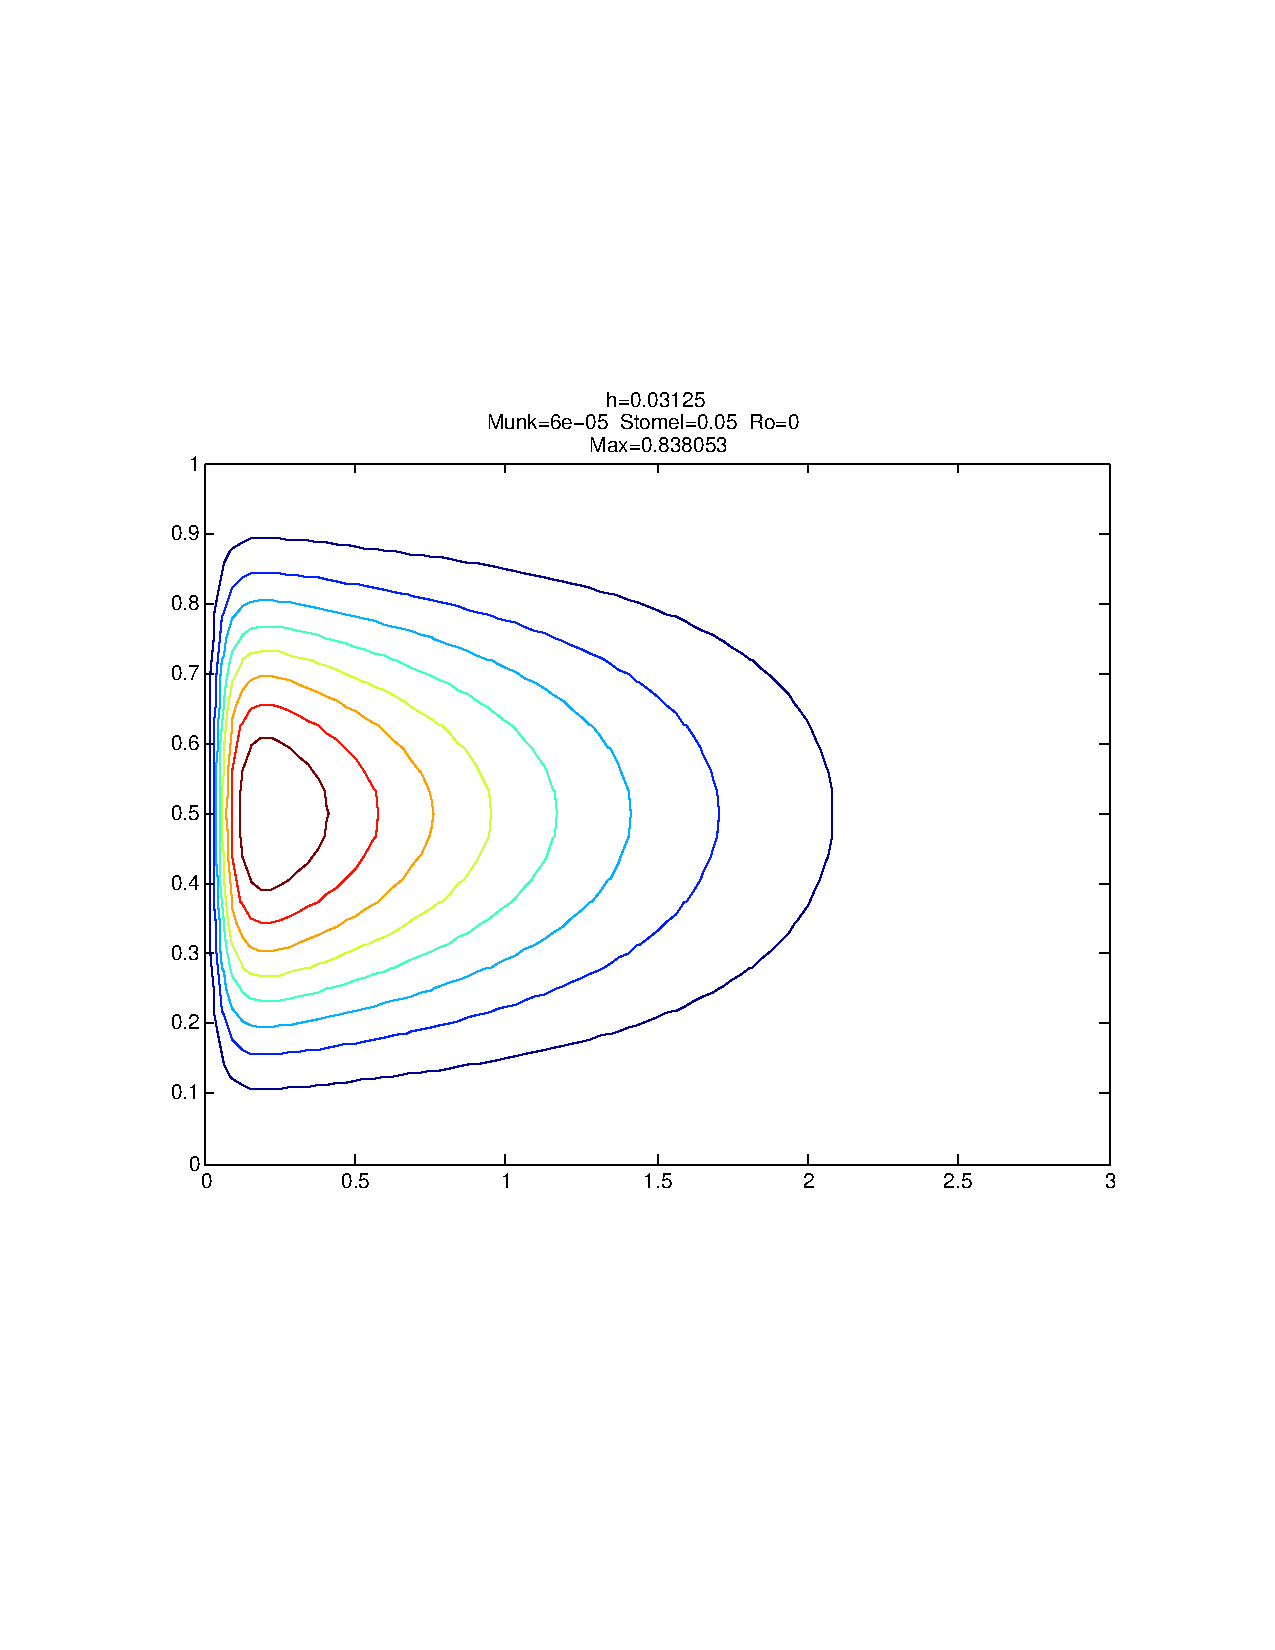
\includegraphics[trim=0 200 20 220, clip=true, scale=0.5]{StommelMunk2.pdf}
    \caption{Linear Stommel-Munk Model \eqref{eqn:SMProb}, Test 4 \cite{Cascon}: Streamlines of the approximation,
    $\psi^h$, $h=\frac{1}{32}$, and $28550$ DoFs.}
    \label{fig:SMe}
  \end{center}
\end{figure}

We note that the errors in \autoref{tab:SMeErrors} follow the theoretical rates
of convergence predicted by the estimates \eqref{eqn:H2Error} -
\eqref{eqn:L2Error} in \autoref{thm:Errors}. Again, we see that the orders of
convergence in \autoref{tab:SMeErrors} are close to the theoretical ones for the
fine meshes, but not as close for the coarse meshes. As stated previously, we
attribute this to the inaccuracies at the thin boundary layer on the left-hand
side (i.e., at $x=0$). The finer the mesh gets, the better this boundary layer
is captured and the better the numerical accuracy becomes.

\subsection{Stationary Quasigeostrophic Equations}\label{sse:SQGE}
This subsection presents results for the FE discretization of the streamfunction formulation of the
SQGE \eqref{sqge_psi_1} by using the Argyris element. Our computational domain is
$\Omega=[0,3]\times[0,1]$, the Reynolds number is $Re=1.667$, and the Rossby number is $Ro=10^{-4}$.
For completeness, we present results for two numerical tests, denoted by Test 5 and Test 6, both
corresponding to the exact solutions given in Test 1 and Test 2 of \cite{Cascon}, respectively.

\tbf{Test 5:}
In this test, we take the same exact solution presented in \emph{Test 3}, i.e.
\begin{equation}
  \psi(x,y) = \sin^2 \frac{\pi x}{3} \cdot \sin^2 \pi y.
  \label{eqn:StreamfunctionExact1}
\end{equation}
Again, the forcing term $F$ and homogeneous boundary conditions, $\psi = \frac{\partial
\psi}{\partial \mathbf{n}} = 0$, correspond to the exact solution \eqref{eqn:StreamfunctionExact1}.

\autoref{fig:SQGEsin} presents the streamlines of the approximate solution obtained by using the
Argyris Finite Element on a mesh with $h=\frac{1}{32}$ and $28550$ DoFs. We note that the
streamlines look as we expect and are similar to those given by Figure $7$ in \cite{Myers}, which
uses the same exact solution.  Since the exact solution is available, we can compute the errors in
various norms. \autoref{tab:SQGEsinErrors} presents the errors $e_0,\, e_1, \text{ and } e_2$ (i.e.,
the $L^2,\, H^1, \text{ and } H^2$ errors, respectively) for various values of the mesh sizes, $h$.

\begin{table}%[H]
\begin{center}
%{\scriptsize
\begin{tabular}{|c|c|c|c|c|c|c|c|}%c|c|}
  \hline
  $h$ & $DoFs$ & $e_0$ & $L_2$ order & $e_1$ & $H^1$ order & $e_2$ & $H^2$ order \\[0.2em] % & $e_{\infty}$ & $L_{\infty}$ order \\
  \hline
  $\nicefrac{1}{2}$ & $170$ & $0.005709$ & $-$ & $0.06033$ & $-$ & $1.087$ & $-$ \\[0.2em] % & $0.007512$ & $-$ \\
  $\nicefrac{1}{4}$ & $550$ & $3.726\times 10^{-5}$ & $7.259$ & $0.001086$ & $5.796$ & $0.04113$ & $4.724$ \\[0.2em] % & $2.828\times 10^{-5}$ & $8.053$ \\
  $\nicefrac{1}{8}$ & $1958$ & $3.597\times 10^{-7}$ & $6.695$ & $2.534\times 10^{-5}$ & $5.421$ & $0.002252$ & $4.191$ \\[0.2em] % & $3.488\times 10^{-7}$ & $6.341$ \\
  $\nicefrac{1}{16}$ & $7366$ & $4.648\times 10^{-9}$ & $6.274$ & $7.065\times 10^{-7}$ & $5.165$ & $0.0001344$ & $4.067$\\[0.2em] % & $4.696\times 10^{-9}$ & $6.215$ \\
  $\nicefrac{1}{32}$ & $28550$ & $6.737\times 10^{-11}$ & $6.108$ & $2.116\times 10^{-8}$ & $5.061$ & $8.26\times 10^{-6}$ & $4.024$ \\[0.2em] % & $6.965\times 10^{-11}$ & $6.075$ \\
 \hline
\end{tabular}
%}
\end{center}
\caption{Errors and Rate of Convergence for the Full SQGE \eqref{sqge_psi_1}, Test 5}
\label{tab:SQGEsinErrors}
\end{table}

\begin{figure}%[H]
  \begin{center}
    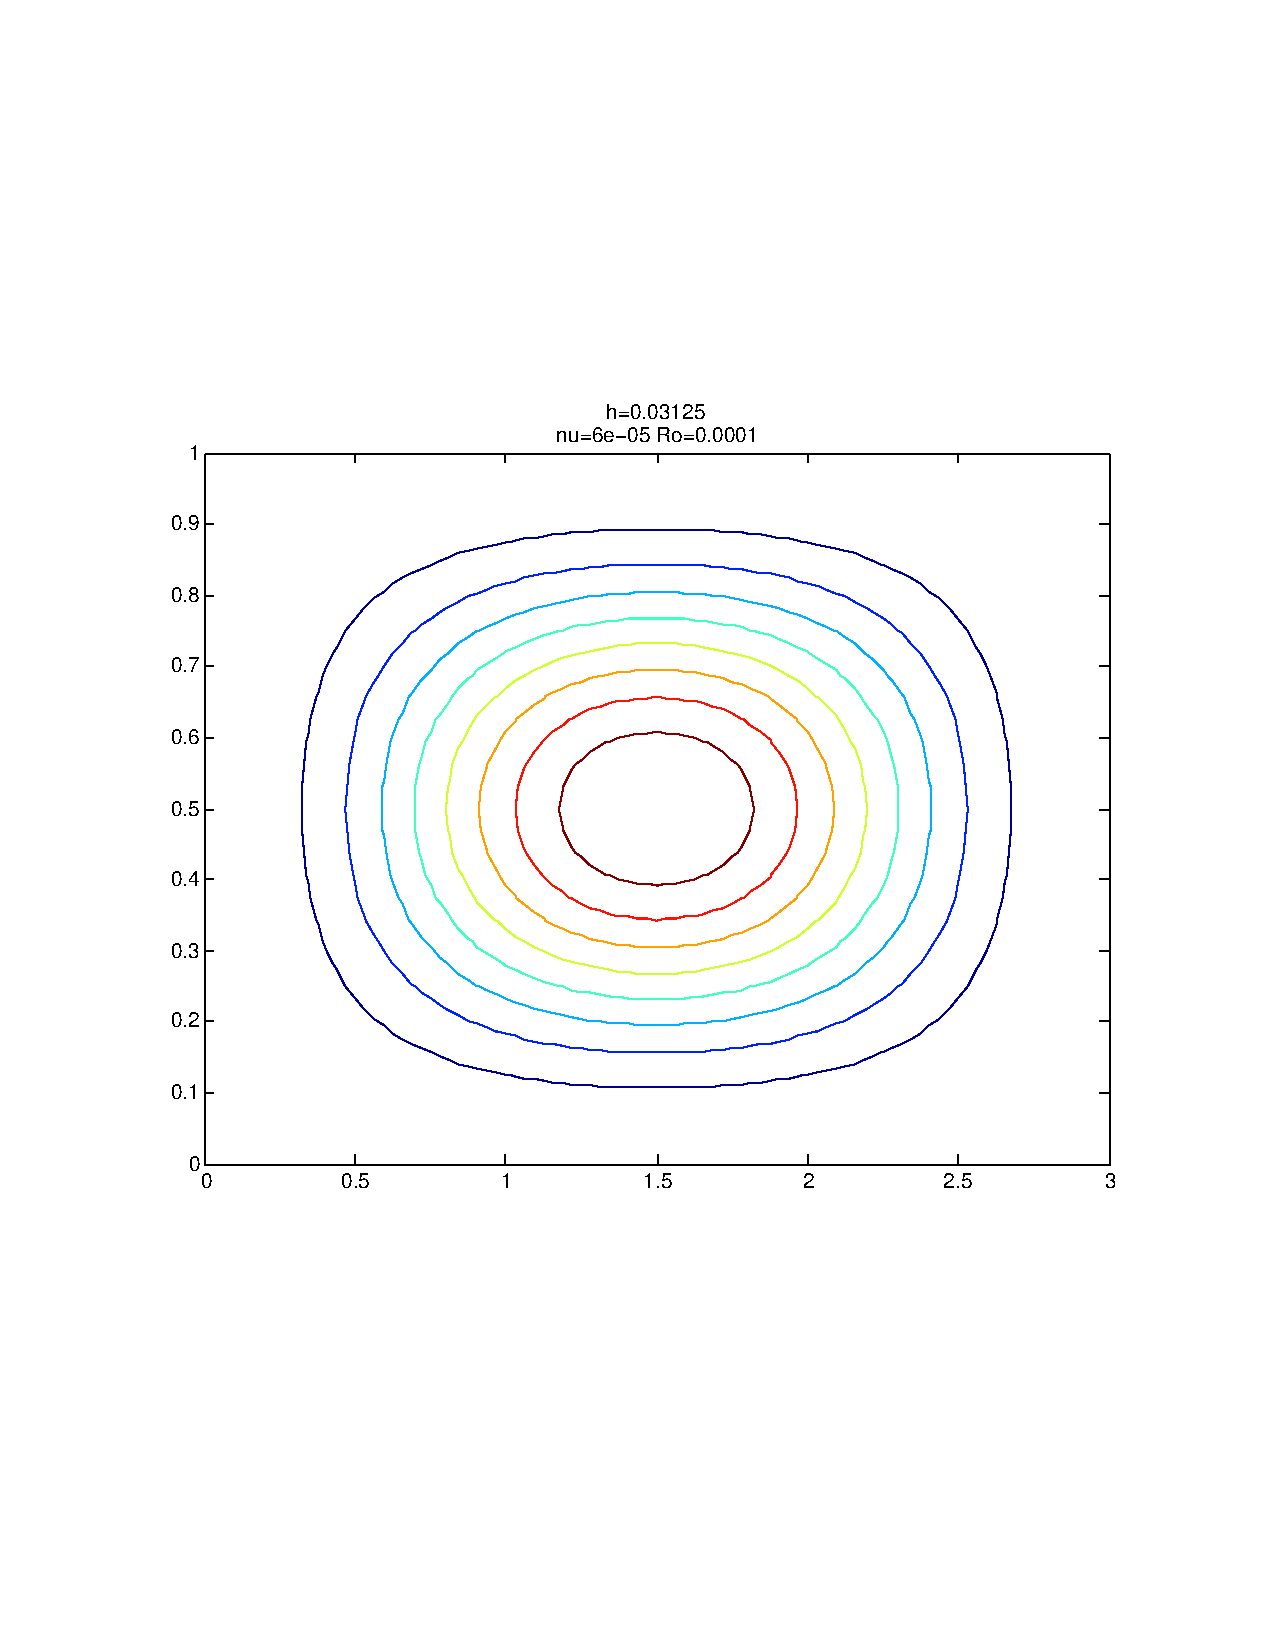
\includegraphics[trim=0 200 20 215, clip=true, scale=0.5]{SQGEsin.pdf}
    \label{fig:SQGEsin}
    \caption{Full SQGE \eqref{sqge_psi_1}, Test 5: Streamlines of the approximation,
    $\psi^h$, $h=\frac{1}{32}$, and $28550$ DoFs.}
  \end{center}
\end{figure}

We note that the errors in \autoref{tab:SQGEsinErrors} follow the theoretical rates of convergence
predicted by the estimates \eqref{eqn:H2Error} - \eqref{eqn:L2Error} in \autoref{thm:Errors}. Again,
since the exact solution \eqref{eqn:StreamfunctionExact1} does not display any boundary layers, we
see that the orders of convergence in \autoref{tab:SQGEsinErrors} are close to the theoretical ones for the fine meshes, but are higher
than expected for the for the coarse meshes.

\tbf{Test 6:}
In this test, we take the same exact solution as used in \emph{Test 4}, i.e.
\begin{equation}
  \psi(x,y) = \left[\left(1 - \frac{x}{3}\right)\left(1-e^{-20x}\right) \sin \pi y\right]^2.
  \label{eqn:StreamfunctionExact2}
\end{equation}
The forcing term $F$ and the homogeneous boundary conditions correspond to the exact solution
\eqref{eqn:StreamfunctionExact2}.

\autoref{fig:SQGEe} presents the streamlines of the approximate solution obtained by using the
Argyris Finite Element on a mesh with $h=\frac{1}{32}$ and $28550$ DoFs. We note that the
streamlines look as we expect and are similar to those given by Figure $10$ in \cite{Myers}, which
uses the same exact solution. Since the exact solution is available, we can compute the errors in
various norms. \autoref{tab:SQGEeErrors} presents the errors $e_0,\, e_1, \text{ and } e_2$ (i.e.,
the $L^2,\, H^1, \text{ and } H^2$ errors, respectively) for various values of the mesh sizes, $h$.

\begin{table}%[H]
\begin{center}
%{\small
\begin{tabular}{|c|c|c|c|c|c|c|c|}%c|c|}
  \hline
  $h$ & $DoFs$ & $e_0$ & $L_2$ order & $e_1$ & $H^1$ order & $e_2$ & $H^2$ order \\[0.2em] % & $e_{\infty}$ & $L_{\infty}$ order \\
  \hline
  $\nicefrac{1}{2}$ & $170$ & $0.3497$ & $-$ & $1.9$ & $-$ & $44.05$ & $-$ \\[0.2em] % & $0.353$ & $-$ \\
  $\nicefrac{1}{4}$ & $550$ & $0.0302$ & $3.533$ & $0.4279$ & $2.15$ & $21.74$ & $1.019$ \\[0.2em] % & $0.03188$ & $3.469$ \\
  $\nicefrac{1}{8}$ & $1958$ & $0.001507$ & $4.324$ & $0.06085$ & $2.814$ & $5.661$ & $1.941$ \\[0.2em] % & $0.002121$ & $3.91$ \\
  $\nicefrac{1}{16}$ & $7366$ & $3.225\times 10^{-5}$ & $5.547$ & $0.004042$ & $3.912$ & $0.7379$ & $2.94$ \\[0.2em] % & $3.832\times 10^{-5}$ & $5.79$ \\
  $\nicefrac{1}{32}$ & $28550$ & $5.672\times 10^{-7}$ & $5.829$ & $0.000161$ & $4.65$ & $0.0597$ & $3.628$ \\[0.2em] % & $8.91\times 10^{-7}$ & $5.426$ \\
 \hline
\end{tabular}
%}
\end{center}
\caption{Errors and Rate of Convergence for the Full SQGE \eqref{sqge_psi_1}, Test 6}
\label{tab:SQGEeErrors}
\end{table}

\begin{figure}%[H]
  \begin{center}
    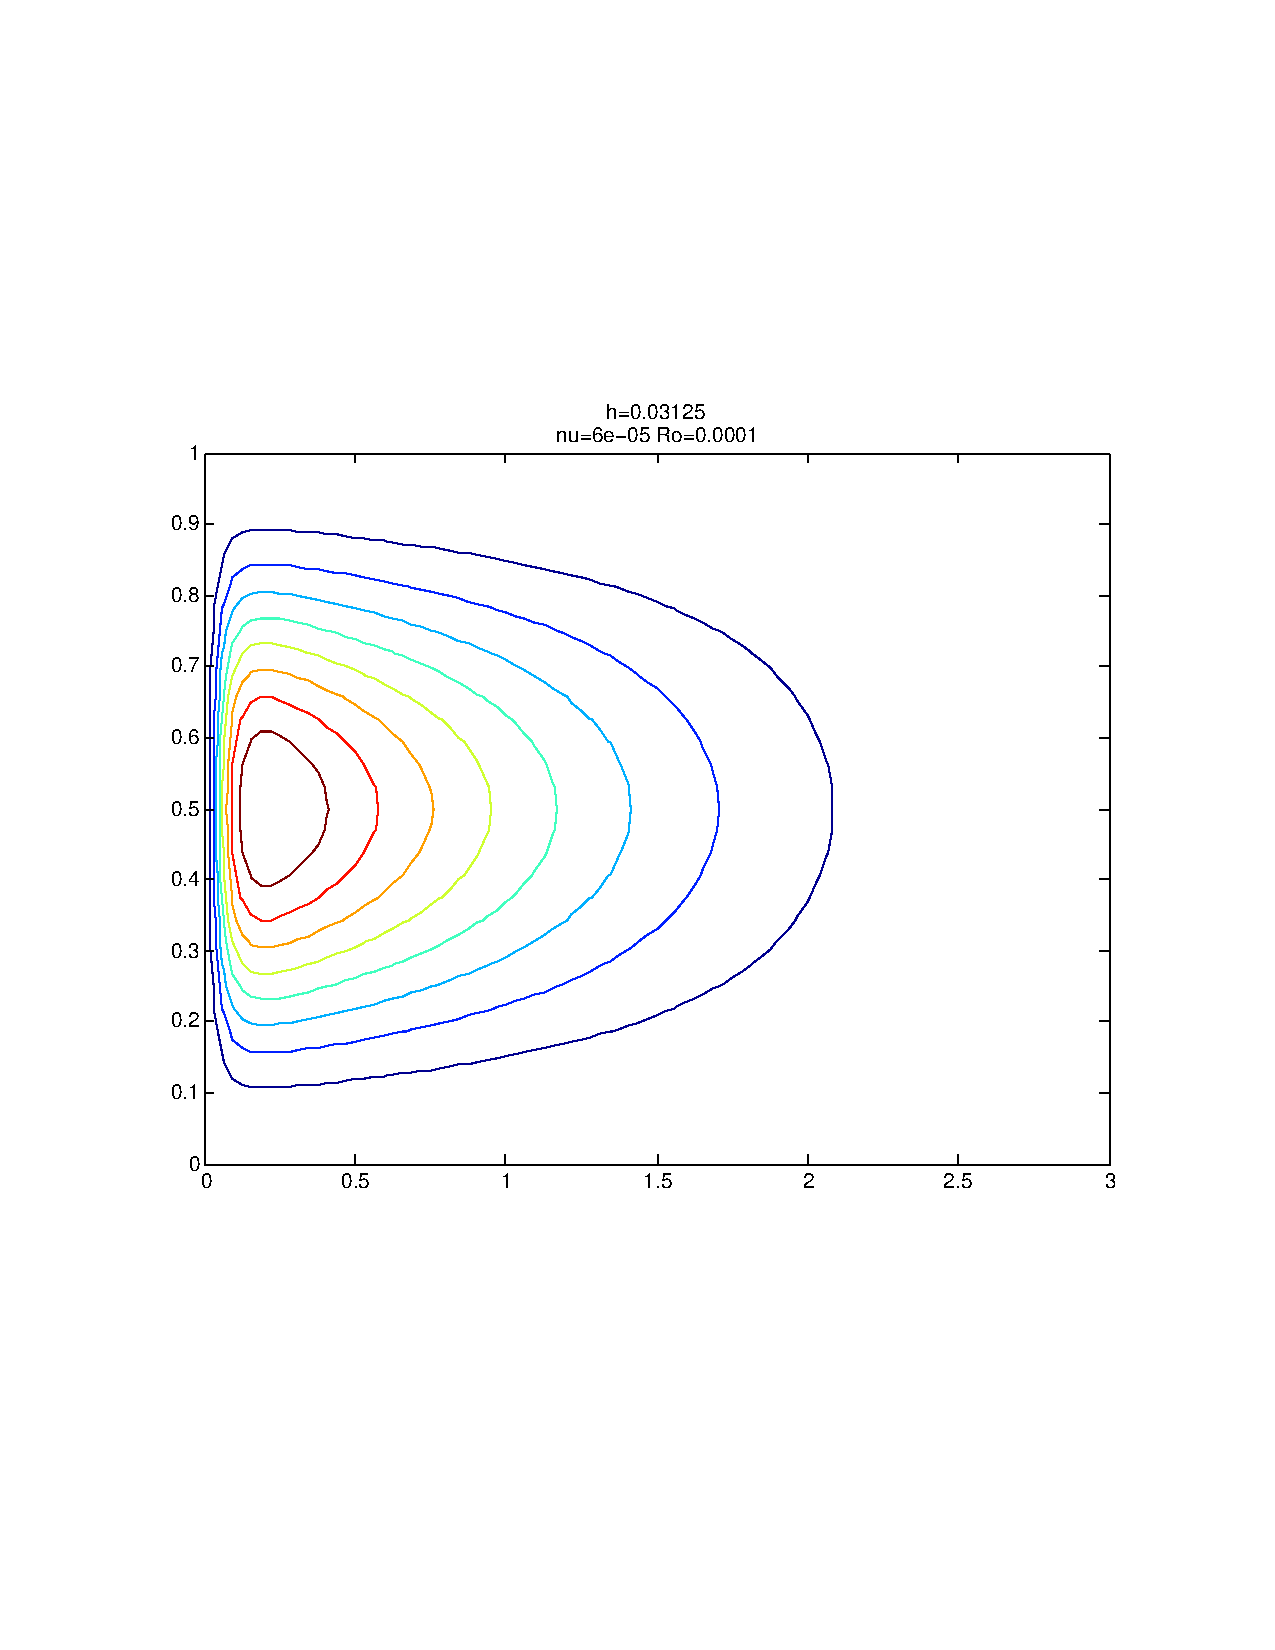
\includegraphics[trim=0 200 20 215, clip=true, scale=0.5]{SQGEe.pdf}
    \caption{Full SQGE \eqref{sqge_psi_1}, Test 6: Streamlines of the approximation,
    $\psi^h$, $h=\frac{1}{32}$, and $28550$ DoFs.}
    \label{fig:SQGEe}
  \end{center}
\end{figure}

We note that the errors in \autoref{tab:SQGEeErrors} follow the theoretical rates of convergence
predicted by the estimates \eqref{eqn:H2Error} - \eqref{eqn:L2Error} in \autoref{thm:Errors}. Again
for an exact solution which has a western boundary layer, we see that the orders of convergence in \autoref{tab:SQGEeErrors} are close to the theoretical ones for the fine meshes, but
not as close for the coarse meshes. We attribute this to the inaccuracies at the thin boundary layer
on the left-hand side (i.e., at $x=0$). The finer the mesh gets, the better this boundary layer is
captured and the better the numerical accuracy becomes.

    \section{SQGE Two-Level} \label{sec:SQGE2LTests}
    The main goal of this section is to verify the theoretical rates of convergence developed in
\autoref{sse:SQGE2LE} by comparing with the observed rates of convergence in our numerical tests.
%Additonally, we intend to demonstrate the time savings from applying the Two-Level method to the
%SQGE. To demonstrate that the two-level method is an affective way to address computational time we
%must demonstrate that the error is at least the same order of convergence as the FE applied to SQGE
%without the two-level method, or we must demonstrate that the cost of using a finer mesh that will
%produce the same level of accuracy is still cheaper computationally.
Unlike the previous section, for the two-level method we must demonstrate rates of convergence for
two different meshes, the fine mesh, $h$, and the coarse mesh $H$. Since the error corresponding to
the coarse mesh dominates the error corresponding to the fine mesh the rate of convergence in the
coarse mesh is easy to demonstrate. To this end one need only pick a constant fine mesh and then
refine the coarse mesh. By doing this one is able to demonstrate the rate of convergence in the
coarse mesh. However, the rate of convergence in the fine mesh is a bit more trick to demonstrate,
because as stated previously the coarse mesh error dominates the fine mesh error and therefore one
must balance the error between the fine mesh and the coarse mesh so as to be able to demonstrate the
rate of convergence in the fine mesh. To this end we set the error terms in
\eqref{eqn:TwoLevelError} equal to eachother to come up with the relationship 
\begin{equation}
  h = \left(\ln h\right)^{\frac{1}{8}} H^{\frac{5}{4}}.
  \label{eqn:OrderRelation}
\end{equation}
This relation is super linear and essentially means that the coarse mesh $H$ must be about half the
size the fine mesh $h$. 

To this end we apply the Two-Level method to the SQGE \eqref{sqge_psi_1} with $Re=Ro=1$ and exact
solution
\begin{equation}
  \left(\sin 4\pi x \cdot \sin 2\pi y\right)^2.
  \label{eqn:2LExact}
\end{equation}
Additionally, the homogeneous boundary conditions are $\psi=\dfrac{\partial \psi}{\partial
\mathbf{n}}=0$ and the forcing function $F$ corresponds to applying the SQGE to the exact solution
\eqref{eqn:2LExact}. Theses BCs and exact solution will be used in all the Two-Level tests that
follow.

First, we benchmark our numerical tests by running SQGE without the two-level method. Comparing to
this benchmark will allows us to compare errors in the $H^2$ norm for SQGE to the errors in $H^2$
norm with the two-level method applied.
\begin{table}[H]
  \begin{center}
  \begin{tabular}{|c|c|c|c|c|}
    \hline
    $h$ & $DoFs$ & $e_2$ & $H^2$ order & time (s) \\
    \hline
    $\nicefrac{1}{2}$ & $70$ & $174.5$ & $-$ & $0.70114$ \\[0.2em] 
    $\nicefrac{1}{4}$ & $206$ & $45.11$ & $1.951$ & $0.63921$ \\[0.2em] 
    $\nicefrac{1}{8}$ & $694$ & $9.286$ & $2.28$ & $3.3169$ \\[0.2em] 
    $\nicefrac{1}{16}$ & $2534$ & $0.6503$ & $3.836$ & $15.105$ \\[0.2em] 
    $\nicefrac{1}{32}$ & $9670$ &  $0.03566$ & $4.189$ & $66.037$ \\[0.2em] 
    $\nicefrac{1}{64}$ & $37766$ & $0.002109$ & $4.08$ & $303.05$ \\[0.2em]
    \hline
  \end{tabular}
  \caption{Benchmark Errors and Rate of Convergence SQGE \eqref{sqge_psi_1}.}
  \label{tab:2LBenchmark}
  \end{center}
\end{table}
As can be seen in \autoref{tab:2LBenchmark} the initial error is quite large in the $H^2$
norm. This is due to lack of resolution in the approximate solution because of the mesh coarseness.
The given exact solution \eqref{eqn:2LExact} has a period of $\dfrac{1}{2}$ in the $x$-direction and
a period of one in the $y$-direction, therefore we must have a mesh size that much smaller than
$\dfrac{1}{2}$ to be able to approximate the function appropriately. However, we see that by
$h=\dfrac{1}{64}$ the error has on the order of $10^{-3}$ and the rate of convergence matches the
theoretical rate of convergence predicted in \autoref{sec:QGEError}.

\begin{table}[H]
  \begin{center}
  \begin{tabular}{|c|c|c|c|c|c|}
    \hline
    $H$ & $DoFs$ for $H$ & $h$ & $DoFs$ for $h$ & $e_2$ & $H^2$ order \\
    \hline
    $\nicefrac{1}{2}$ & $70$ & $\nicefrac{1}{4}$ & $206$ & $45.44$ & $-$ \\[0.2em] 
    $\nicefrac{1}{4}$ & $206$ & $\nicefrac{1}{8}$ & $694$ & $10.89$ & $2.061$ \\[0.2em] 
    $\nicefrac{1}{8}$ & $694$ &$\nicefrac{1}{16}$ & $2534$ & $0.8404$ & $3.696$ \\[0.2em] 
    $\nicefrac{1}{16}$ & $2534$ & $\nicefrac{1}{32}$ & $9670$ & $0.04075$ & $4.366$ \\[0.2em] 
    $\nicefrac{1}{32}$ & $9670$ & $\nicefrac{1}{64}$ & $37766$ &  $0.002141$ & $4.25$ \\[0.2em] 
    $\nicefrac{1}{64}$ & $37766$ & $\nicefrac{1}{128}$ & $149254$ & $0.0001298$ & $4.044$ \\[0.2em]
    \hline
  \end{tabular}
  \caption{Errors and Rate of Convergence in $h$ for the Two-Level method applied to SQGE \eqref{sqge_psi_1}.}
  \label{tab:TwoLevelh}
  \end{center}
\end{table}

In \autoref{tab:TwoLevelh} we use the relationship \eqref{eqn:OrderRelation} to determine a mesh
size relationship between $h$ and $H$. As stated previously, this relation implies that $H \approx
\dfrac{h}{2}$ and therefore we chose the $(H,h)$ pairs corresponding to 
\begin{equation*}
  \left\{ \left(\frac{1}{2}, \frac{1}{4}\right),
  \left(\frac{1}{4}, \frac{1}{8}\right),
  \left(\frac{1}{8}, \frac{1}{16}\right),
  \left(\frac{1}{16}, \frac{1}{32}\right),
  \left(\frac{1}{32}, \frac{1}{64}\right),
  \left(\frac{1}{64}, \frac{1}{128}\right)\right\}
\end{equation*}
so as to demonstrate the rate of convergence in $h$. As can be seen in \autoref{tab:TwoLevelh} the
rate of convergence does, in deed, approach the rate of convergence predicted in
\autoref{sse:SQGE2LE}. Additionally, we see that the $H^2$ errors are of the same order
as the corresponding errors in \autoref{tab:2LBenchmark} for the same value of $h$.

To demonstrate the rate of convergence in $H$ we take a constant fine mesh size of
$h=\dfrac{1}{128}$ and vary the coarse mesh $H$. To this end we chose the $(H,h)$ pairs
corresponding to 
\begin{equation*}
  \left\{ \left(\frac{1}{2}, \frac{1}{128}\right),
  \left(\frac{1}{4}, \frac{1}{128}\right),
  \left(\frac{1}{8}, \frac{1}{128}\right),
  \left(\frac{1}{16}, \frac{1}{128}\right),
  \left(\frac{1}{32}, \frac{1}{128}\right),
  \left(\frac{1}{64}, \frac{1}{128}\right)\right\}.
\end{equation*}

\begin{table}[H]
  \begin{center}
  \begin{tabular}{|c|c|c|c|c|c|}
    \hline
    $H$ & $DoFs$ for $H$ & $h$ & $DoFs$ for $h$ & $e_2$ & $H^2$ order \\
    \hline
    $\nicefrac{1}{2}$ & $70$ & $\nicefrac{1}{128}$ & $149254$ & $7.653$ & $-$ \\[0.2em] 
    $\nicefrac{1}{4}$ & $206$ & $\nicefrac{1}{128}$ & $149254$ & $5.916$ & $0.3715$ \\[0.2em] 
    $\nicefrac{1}{8}$ & $694$ & $\nicefrac{1}{128}$ & $149254$ & $0.5373$ & $3.461$ \\[0.2em] 
    $\nicefrac{1}{16}$ & $2534$ & $\nicefrac{1}{128}$ & $149254$ & $0.0199$ & $4.755$ \\[0.2em] 
    $\nicefrac{1}{32}$ & $9670$ & $\nicefrac{1}{128}$ & $149254$ &  $0.0003779$ & $5.719$ \\[0.2em] 
    $\nicefrac{1}{64}$ & $37766$ & $\nicefrac{1}{128}$ & $149254$ & $1.381\times 10^{-5}$ & $4.775$ \\[0.2em]
    \hline
  \end{tabular}
  \caption{Errors and Rate of Convergence in $H$ for the Two-Level method applied to SQGE \eqref{sqge_psi_1}.}
  \label{tab:TwoLevelH}
  \end{center}
\end{table}

As can be seen in \autoref{tab:TwoLevelH} the rate of convergence does, in deed, approach the rate
of convergence predicted in \autoref{sse:SQGE2LE}. Additionally, we see that the $H^2$ errors are of
the same order as the corresponding errors in \autoref{tab:2LBenchmark} for the same value of $h$.

%Finally, to demonstrate the computational efficiency of the two-level method we compare the time
%required to run simulations for the SQGE with out the two-level method on various mesh sizes and
%then we simulate the SQGE with the two-level method for the same fine mesh size as those used in the
%non two-level method, while maintaining the same coarse mesh size accross all simulations. For these
%simulations we will take the coarse mesh to be $H=\dfrac{1}{2}$ and vary the fine mesh $h$ over 
%\begin{equation*}
%  \left\{\frac{1}{2}, \frac{1}{4}, \frac{1}{8}, \frac{1}{16}, \frac{1}{32}, \frac{1}{64}\right\}.
%\end{equation*}
%
%\begin{table}[H]
%  \begin{center}
%  \begin{tabular}{|c|c|c|c|c|c|c|}
%    \hline
%    $H$ & $DoFs$ for $H$ & $h$ & $DoFs$ for $h$ & $e_2$ & $H^2$ order & time (s) \\
%    \hline
%    $\nicefrac{1}{2}$ & $70$ & $\nicefrac{1}{2}$ & $70$ & $174.55$ & $-$ & $0.2287$ \\[0.2em] 
%    $\nicefrac{1}{2}$ & $70$ & $\nicefrac{1}{4}$ & $206$ & $45.44$ & $1.941$ & $0.2898$ \\[0.2em] 
%    $\nicefrac{1}{2}$ & $70$ &$\nicefrac{1}{8}$ & $694$ & $11.99$ & $ 1.922$ & $0.6902$ \\[0.2em] 
%    $\nicefrac{1}{2}$ & $70$ & $\nicefrac{1}{16}$ & $2534$ & $7.681$ & $0.6431$ & $2.803$ \\[0.2em] 
%    $\nicefrac{1}{2}$ & $70$ & $\nicefrac{1}{32}$ & $9670$ &  $7.653$ & $0.00511$ & $12.75$ \\[0.2em] 
%    $\nicefrac{1}{2}$ & $70$ & $\nicefrac{1}{64}$ & $37766$ & $7.653$ & $1.526\times 10^{-5}$ & $58.67$ \\[0.2em]
%    \hline
%  \end{tabular}
%  \caption{Errors and Rate of Convergence in $H$ for the Two-Level method applied to SQGE \eqref{sqge_psi_1}.}
%  \label{tab:TwoLevelH}
%  \end{center}
%\end{table}

    \section{QGE} \label{sec:QGETests}
    \subsection{Verification of Rates of Convergence}
In this subsection we verify the theoretical error estimates developed in
\autoref{sec:QGEError}. To this end, we apply the Argyris FE in space while
applying implicit Euler in time to \eqref{eqn:QGE_psi}. To solve the resulting
nonlinear system at each time step we apply Newton's method where the Newton's
method is considered to have converged when the $L^2$-norm of the difference in
the current Newton iterate and the previous Newton iterate is less than
$10^{-7}$. Additionally, in each of the following computational tests we take
$Re = 1$, $Ro = 1$, and $h = \nicefrac{1}{20}$ unless otherwise stated.

\subsubsection*{Test 1}
For this test we take the exact solution to be
\begin{equation}
  \psi(t;x,y) = \left(\sin \pi x \sin \pi y\right)^2 \sin t
  \label{eqn:Test1}
\end{equation}
which is very similar to \textbf{Test 6} in \cite{Foster}. Here we add the time
dependence in the sine term and let $\Omega = [0,1]^2$. The time interval for
integration is $t = [0,\frac{\pi}{2}]$. This test will have an intensifying
western boundary layer as time increases.

\begin{table}
  \begin{center}
    \begin{tabular}{|c|c|c|c|c|}
      \hline
      $k$ & $h$ & DoFs & $e_{L^2}$ & $L^2$ order \\% & $e_{H^1}$ & $H^1$ order & $e_{H^2}$ & $H^2$ order \\
      \hline
      $\nicefrac{1}{2}$ & $\nicefrac{1}{16}$ & $2853$ & $5.65\times 10^{-4}$ & $-$ \\%& $0.00293$ & $-$ & $0.01971$ & $-$ \\
      $\nicefrac{1}{4}$ & $\nicefrac{1}{16}$ & $2853$ & $3.49\times 10^{-4}$ & $0.697$ \\%& $0.001807$ & $0.6971$ & $0.01216$ & $0.697$ \\
      $\nicefrac{1}{8}$ & $\nicefrac{1}{16}$ & $2853$ & $1.916\times 10^{-4}$ & $0.864$ \\%& $0.0009931$ & $0.8636$ & $0.006683$ & $0.8634$ \\
      $\nicefrac{1}{16}$ & $\nicefrac{1}{16}$ & $2853$ & $1.001\times 10^{-4}$ & $0.937$ \\%& $0.0005189$ & $0.9366$ & $0.003494$ & $0.9359$ \\
      $\nicefrac{1}{32}$ & $\nicefrac{1}{16}$ & $2853$ & $5.11\times 10^{-5}$ & $0.970$ \\%& $0.000265$ & $0.9696$ & $0.001787$ & $0.9668$ \\
      $\nicefrac{1}{64}$ & $\nicefrac{1}{16}$ & $2853$ & $2.58\times 10^{-5}$ & $0.985$ \\%& $0.0001339$ & $0.9851$ & $0.0009098$ & $0.9743$ \\
      $\nicefrac{1}{128}$ & $\nicefrac{1}{16}$ & $2853$ & $1.30\times 10^{-5}$ & $0.993$ \\%& $6.728\times 10^{-5}$ & $0.9925$ & $0.0004705$ & $0.9513$ \\
      $\nicefrac{1}{256}$ & $\nicefrac{1}{16}$ & $2853$ & $6.51\times 10^{-6}$ & $0.996$ \\%& $3.374\times 10^{-5}$ & $0.9959$ & $0.0002607$ & $0.8516$ \\
      $\nicefrac{1}{512}$ & $\nicefrac{1}{16}$ & $2853$ & $3.26\times 10^{-6}$ & $0.998$ \\%& $1.691\times 10^{-5}$ & $0.9965$ & $0.0001715$ & $0.6046$ \\
      $\nicefrac{1}{1024}$ & $\nicefrac{1}{16}$ & $2853$ & $1.63\times 10^{-6}$ & $0.999$ \\%& $8.497\times 10^{-6}$ & $0.9927$ & $0.0001405$ & $0.2878$ \\
      \hline

    \end{tabular}
  \end{center}
  \caption{Observed order of convergence for Implicit-Euler applied to
    \eqref{eqn:QGE_psi} with the exact solution \eqref{eqn:Test1}.
    %Note the observed order of convergence matches the theoretical error estimates developed in \autoref{sec:QGEError}.
  }
  \label{tab:Test1Time}
\end{table}

\begin{figure}
  \begin{center}
    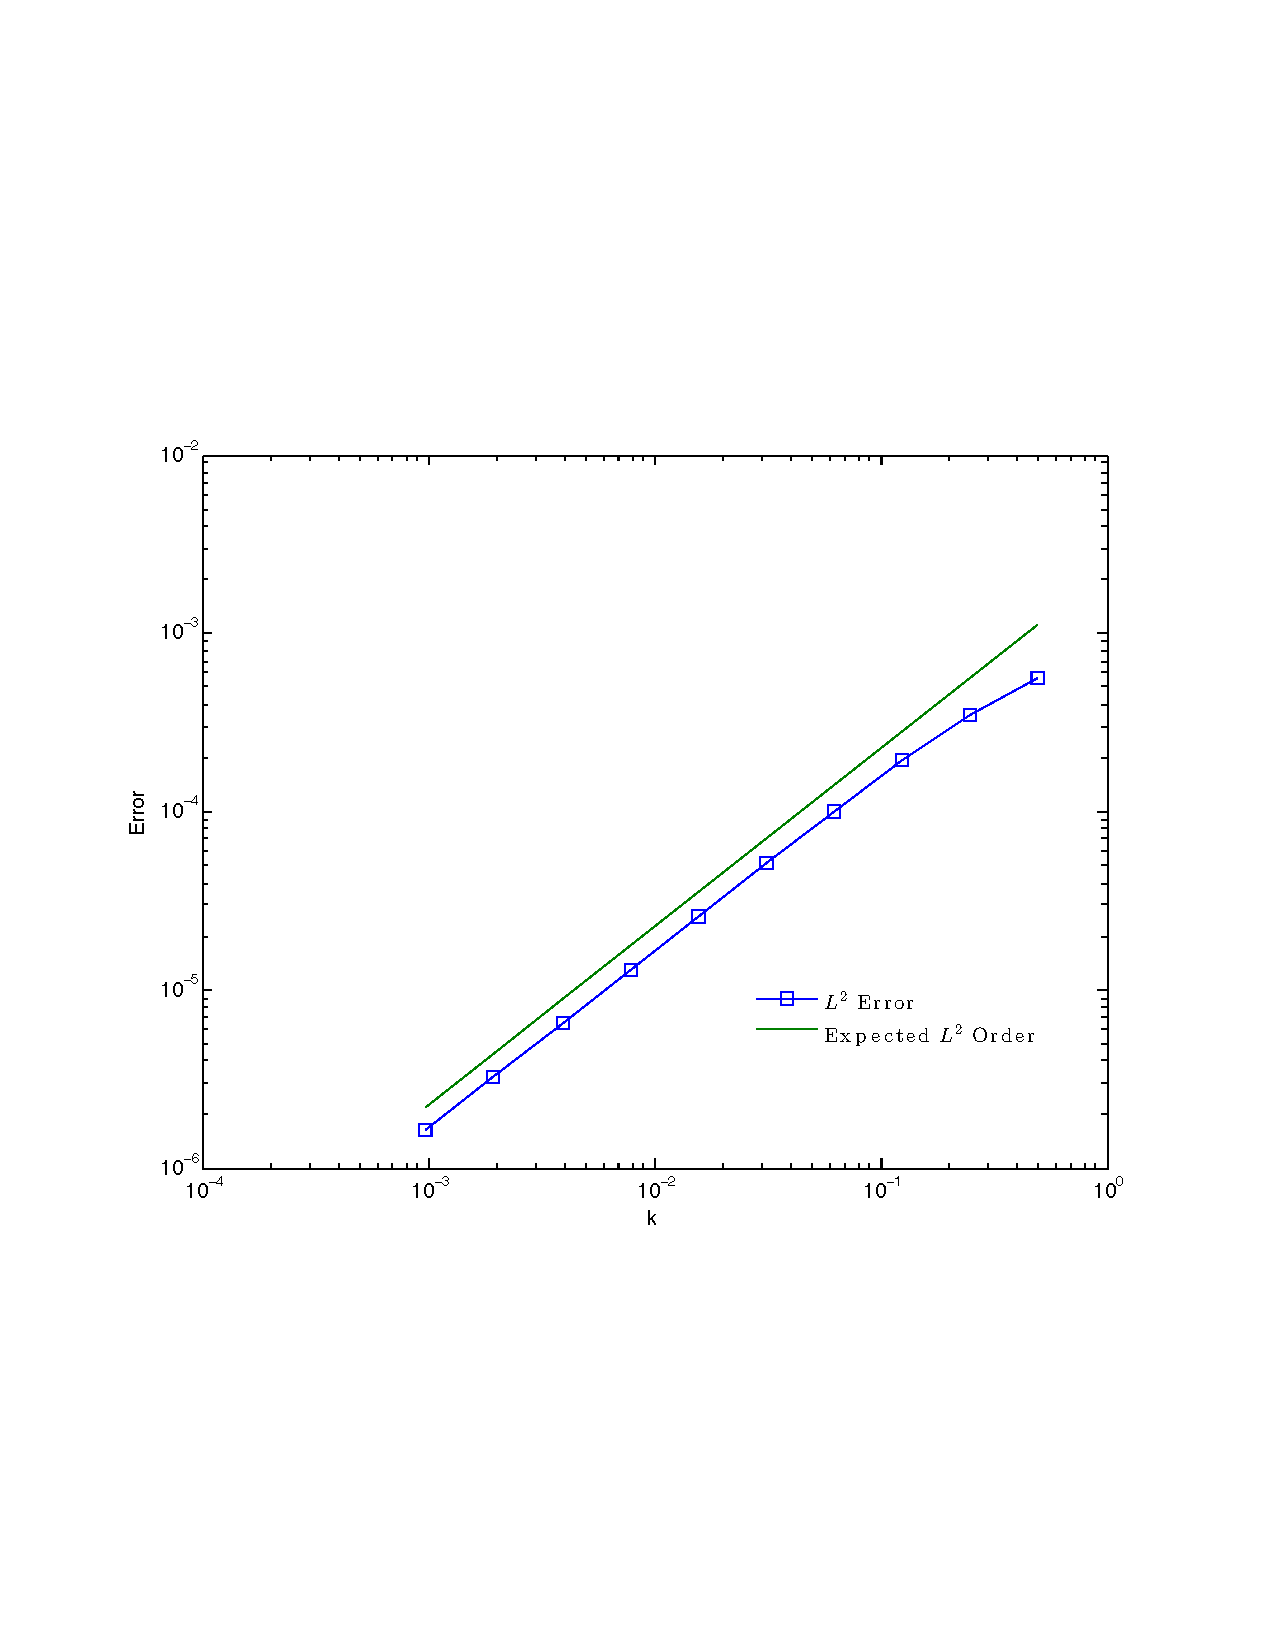
\includegraphics[scale=0.6]{sin2sin2sinTimeConvergence.pdf}
    \caption{Observed order of convergence for Implicit-Euler applied to
      \eqref{eqn:QGE_psi} with the exact solution \eqref{eqn:Test1}.}
  \label{fig:Test1Time}
  \end{center}
\end{figure}

\begin{table}
  \begin{center}
    \begin{tabular}{|c|c|c|c|c|c|c|c|c|}
      \hline
      $k$ & $h$ & DoFs & $e_{L^2}$ & $L^2$ order & $e_{H^1}$ & $H^1$ order & $e_{H^2}$ & $H^2$ order \\
      \hline
      $\nicefrac{1}{8192}$ & $\nicefrac{1}{2}$ & $38$ & $1.23\times 10^{-2}$ & $-$ & $1.18\times 10^{-1}$ & $-$ & $1.57\times 10^0$ & $-$ \\
      $\nicefrac{1}{8192}$ & $\nicefrac{1}{4}$ & $174$ & $2.12\times 10^{-5}$ & $9.18$ & $7.31\times 10^{-4}$ & $7.34$ & $2.79\times 10^{-2}$ & $5.81$ \\
      $\nicefrac{1}{8192}$ & $\nicefrac{1}{8}$ & $662$ & $7.88\times 10^{-7}$ & $4.75$ & $4.59\times 10^{-5}$ & $3.99$ & $3.04\times 10^{-3}$ & $3.20$ \\
      $\nicefrac{1}{8192}$ & $\nicefrac{1}{16}$ & $2853$ & $7.87\times 10^{-9}$ & $6.65$ & $9.05\times 10^{-7}$ & $5.67$ & $1.29\times 10^{-4}$ & $4.56$ \\
      $\nicefrac{1}{8192}$ & $\nicefrac{1}{32}$ & $11690$ & $6.97\times 10^{-11}$ & $6.82$ & $1.88\times 10^{-8}$ & $5.59$ & $5.98\times 10^{-6}$ & $4.43$ \\
      $\nicefrac{1}{8192}$ & $\nicefrac{1}{64}$ & $47958$ & $7.23\times 10^{-12}$ & $3.27$ & $5.26\times 10^{-10}$ & $5.16$ & $3.43\times 10^{-7}$ & $4.12$ \\
      \hline
    \end{tabular}
  \end{center}
  \caption{Observed spatial orders of convergence for Argyris applied to
    \eqref{eqn:QGE_psi} with the exact solution \eqref{eqn:Test2} using implicit
    Euler for time discretization. Note the observed orders of convergence
    nearly matches the theoretical error estimates developed in
    \autoref{sec:QGEError}. The $L^2$ order, however, drops off for the last
    spatial discretization due to nearing the machine epsilon.}
  \label{tab:Test1Space}
\end{table}

\begin{figure}
  \begin{center}
    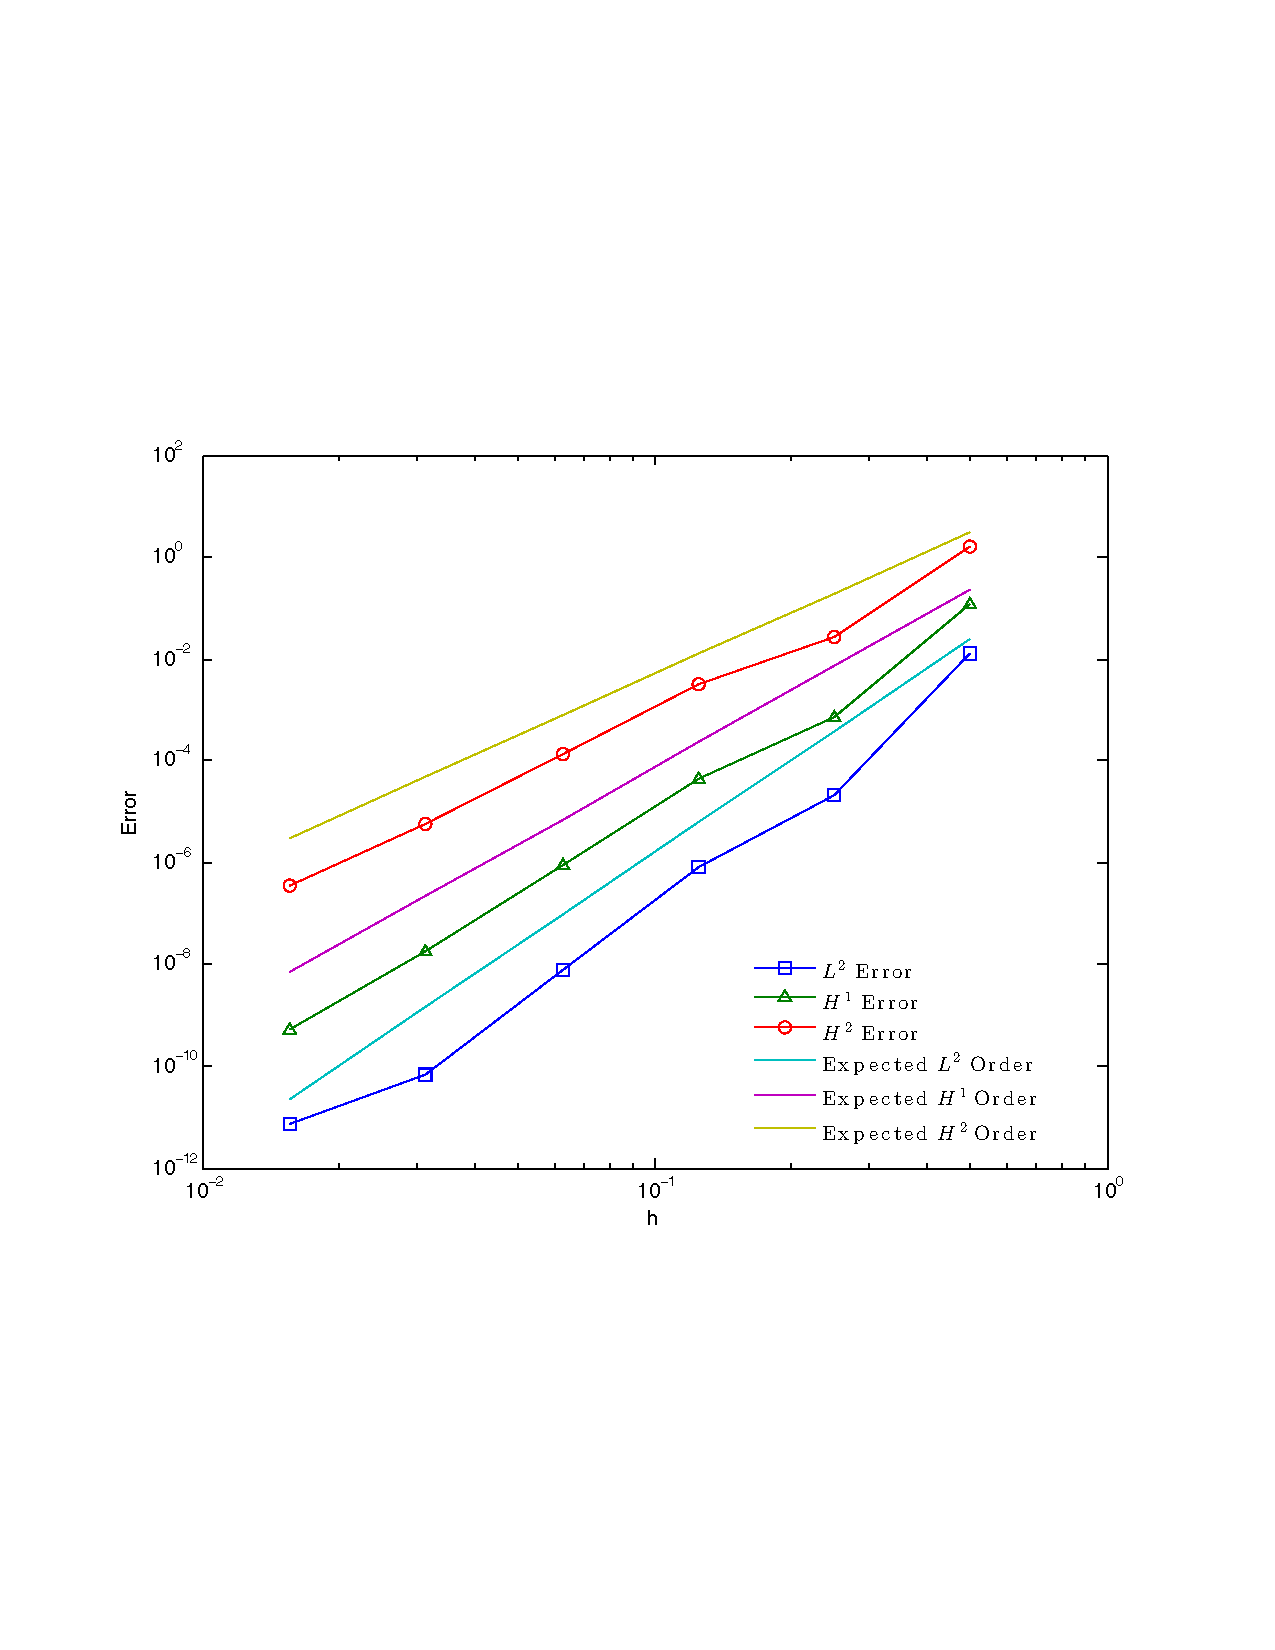
\includegraphics[scale=0.6]{sin2sin2sinSpaceConvergence.pdf}
    \caption{Observed orders of convergence in space for Argyris applied to
      \eqref{eqn:QGE_psi} with the exact solution \eqref{eqn:Test1} using
      implicit Euler for the time discretization.}
  \label{fig:Test1Space}
  \end{center}
\end{figure}

\subsubsection*{Test 2}
For this test we take the exact solution to be
\begin{equation}
  \psi(t;x,y) = \left[(1-x)\left(1-e^{-0.1\,x\,t}\right) \sin \pi y\right]^2
  \label{eqn:Test2}
\end{equation}
which is very similar to \textbf{Test 4} in \cite{Foster}. Here we add the time
dependence in the exponential term and let $\Omega = [0,1]^2$. The time interval
for integration is $t = [0,1]$. This test will have an intensifying western
boundary layer as time increases.
\begin{table}
\begin{center}
  \begin{tabular}{|c|c|c|c|c|}
    \hline
    $k$ & $h$ & DoFs & $e_{L^2}$ & $L^2$ order \\% & $e_{H^1}$ & $H^1$ order & $e_{H^2}$ &         $H^2$ order \\
    \hline
$\nicefrac{1}{8}$ & $\nicefrac{1}{20}$ & $1158$ & $5.00\times 10^{-7}$ & $-$ \\% & $2.576\times 10^{-6}$ & $-$ & $1.738\times 10^{-5}$ & $-$ \\
$\nicefrac{1}{16}$ & $\nicefrac{1}{20}$ & $1158$ & $2.49\times 10^{-7}$ & $1.01$ \\% & $1.284\times 10^{-6}$ & $1.005$ & $8.691\times 10^{-6}$ & $1$ \\
$\nicefrac{1}{32}$ & $\nicefrac{1}{20}$ & $1158$ & $1.24\times 10^{-7}$ & $1.00$ \\% & $6.409\times 10^{-7}$ & $1.002$ & $4.392\times 10^{-6}$ & $0.9846$ \\
$\nicefrac{1}{64}$ & $\nicefrac{1}{20}$ & $1158$ & $6.21\times 10^{-8}$ & $1.00$ \\% & $3.203\times 10^{-7}$ & $1.001$ & $2.299\times 10^{-6}$ & $0.9342$ \\
$\nicefrac{1}{128}$ & $\nicefrac{1}{20}$ & $1158$ & $3.11\times 10^{-8}$ & $1.00$ \\% & $1.602\times 10^{-7}$ & $0.9995$ & $1.337\times 10^{-6}$ & $0.7817$ \\
$\nicefrac{1}{256}$ & $\nicefrac{1}{20}$ & $1158$ & $1.55\times 10^{-8}$ & $1.00$ \\% & $8.034\times 10^{-8}$ & $0.9957$ & $9.564\times 10^{-7}$ & $0.4834$ \\
$\nicefrac{1}{512}$ & $\nicefrac{1}{20}$ & $1158$ & $7.76\times 10^{-9}$ & $1.00$ \\% & $4.068\times 10^{-8}$ & $0.9818$ & $8.346\times 10^{-7}$ & $0.1966$ \\
    \hline
  \end{tabular}
\end{center}
  \caption{Observed order of convergence for Implicit-Euler applied to
    \eqref{eqn:QGE_psi} with the exact solution \eqref{eqn:Test2}. Note the observed
    order of convergence matches the theoretical error estimates developed in
    \autoref{sec:QGEError}.}
  \label{tab:Test2Time}
\end{table}

\subsection{North Atlantic}
The North Atlantic Ocean is intensely studied and therefore makes a good test
problem for evaluating the performance of our model \cite{Myers}. Hence, we have
created a FE mesh of the North Atlantic which extend from $15^\circ N$ to $65^\circ
N$ using GMSH \cite{GMSH}. The coastline data was obtain from GSHHS \cite{GSHHS}.
The finite element spacing was specified to be {\color{red} $15km$}.  Major
islands such as Cuba, Hispaniola Greenland, Great Britain, and Ireland were
connected to the nearest continent and hard boundaries were created at the
northern and southern most extents of the North Atlantic. The resultant FE mesh
can be seen in \autoref{fig:AtlanticMesh}.

\begin{figure}
  \begin{center}
    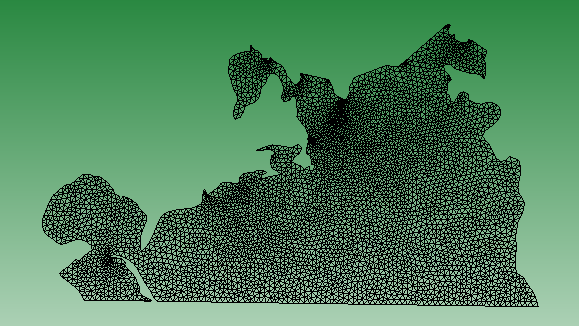
\includegraphics[scale=0.5]{NAMesh.png}
    \caption{Mesh of the North Atlantic created using GMSH \cite{GMSH}.}
    \label{fig:AtlanticMesh}
  \end{center}
\end{figure}

The experiment used annual mean wind forcing obtained from Hellerman and
Rosenstein (1983). We choose similar similar parameters as those used in
\cite{delSastre04} and are summarized in \autoref{tab:AtlanticParameters}.

\begin{table}
  \begin{center}
  \begin{tabular}{|l|l|}
    \hline
    $A$ & $2000m^2s^{-1}$\\
    \hline
    $\theta_0$ & $40^\circ$ \\
    \hline
    $\omega$ & $7.2526\times 10^{-5}s^{-1}$ \\
    \hline
    $H$ & $1000m$ \\
    \hline
    $L$ & $1000km$ \\
    \hline
    $r_e$ & $6378.1km$ \\
    \hline
    $\rho$ & $1027 \nicefrac{kg}{m^3}$ \\
    \hline
  \end{tabular}
  \end{center}
  \caption{Table of parameter values used for the simulations of the North
    Atlantic. \cite{delSastre04}}
  \label{tab:AtlanticParameters}
\end{table}

Using the relation
\begin{equation}
  \beta = \frac{2\omega}{r_e}\cos \theta_0
  \label{eqn:Beta}
\end{equation}
and the parameters given in \autoref{tab:AtlanticParameters} we see that
\begin{equation*}
  \beta \approx 1.742\times 10^{-11}\, m^{-1}\,s^{-1}.
\end{equation*}
Using this approximation for $\beta$ and \eqref{eqn:velocity_scale} with
{\color{red}$\tau_0 = 0.6\, dyne\, cm^{-2}$ \cite{Hellerman} gives the following
approximation for the characteristic velocity
\begin{equation*}
%  \begin{split}
%    U &= \frac{3.1415 \cdot 0.6 dyne\, cm^{-2}}{1027 \nicefrac{kg}{m^3} \cdot
%      1000\, m \cdot 1.742 \times 10^{-11}\,m^{-1}\,s^{-1} \cdot 1000\, km} \\
    U = 1.054\times 10^{-2} \nicefrac{m}{s}.
%  \end{split}
\end{equation*}
Therefore, the Rossby number is
\begin{equation*}
%  Ro = \frac{1.054\times 10^{-2} \nicefrac{m}{s}}{1.742\times 10^{-11} m^{-1}
%    s^{-1} (1000 km)^2}
  Ro = 6.051\times 10^{-4}
\end{equation*}
and the Reynolds number is
\begin{equation*}
  Re = 5.27.
\end{equation*}}

From the length scale $L$ and the velocity scale $U$ we see that the time scale
is approximately $T = 3\, years$. Thus, a nondimensional time interval of
$[0,120]$, which was also used by Bermejo et al \cite{delSastre04}, corresponds
to a total of $360$ years. We use the same dimensional time step used in
\cite{delSastre04}, which was $\Delta t = 2\, hours$. This time step corresponds
to nondimensional time step of $k = 7.6053 \times 10^{-5}$. {\color{red} This
may be unrealistic.}

\subsection{Mediterranean}

\begin{figure}
  \begin{center}
    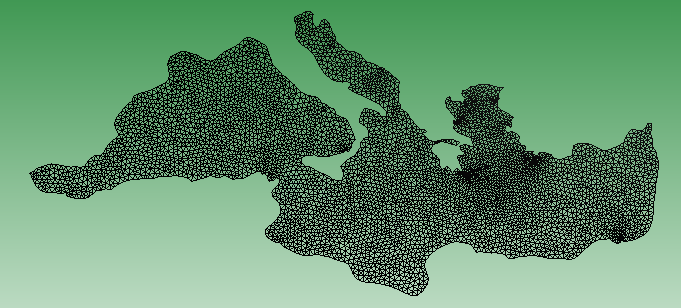
\includegraphics[scale=0.5]{MedMesh.png}
    \caption{Mesh of the Mediterranean created using GMSH \cite{GMSH}.}
    \label{fig:MedMesh}
  \end{center}
\end{figure}



  \chapter{Conclusions} \label{ch:Conclusions}
  \input{Conclusions.tex}

  \bibliographystyle{plain}
  \bibliography{Thesis}

%  \appendix
%  \chapter{Newton Method} \label{sec:Newton}
%  In this section, we briefly outline the implementation details of the Newton
method used to solve the nonlinear system of equations resulting from the FEM
discretization of the streamfunction formulation of the QGE
\eqref{eqn:SemiDiscretization}.

The Newton method is an iterative process that, at each iteration $n$, with $n=1, 2, \dots$ yields an approximation $\psi^h_n$ to the FEM approximation $\psi^h$.
We start the iterative process by making an initial guess $\psi^h_0$.
Given $\psi^h_{n-1}$, the Newton iteration at the previous step, the Newton method computes the current step iteration $\psi^h_n$ according to the following formula:
\begin{eqnarray}
  \left(
  \mathcal{J}(\psi^h_{n-1}) \, \Delta_n \psi^h , \chi^h
  \right)
  &=& -
  \left(
  F(\psi^h_{n-1}) , \chi^h
  \right)
  \qquad
  \forall \, \chi^h \in X^h ,
  \label{eqn:Newton} \\[0.2cm]
  \psi^h_n &=& \Delta_n \psi^h + \psi^h_{n-1},
  \label{eqn:NewPsi}
\end{eqnarray}
where
\begin{eqnarray*}
  \left(
  F(\psi^h_{n-1}) , \chi^h
  \right)
  &=&  a_0(\psi^h_{n-1},\chi^h) + a_1(\psi^h_{n-1},\psi^h_{n-1},\chi^h) + a_2(\psi^h_{n-1},\chi^h) - \ell(\chi^h), \\[0.2cm]
  \left(
  \mathcal{J}(\psi^h_{n-1}) \, \Delta_n \psi^h , \chi^h
  \right)
  &=& a_0(\Delta_n \psi^h,\chi^h)
  + a_1(\Delta_n \psi^h,\psi^h_{n-1},\chi^h)
  \nonumber \\[0.2cm]
  && + a_1(\psi^h_{n-1},\Delta_n \psi^h,\chi^h)
  + a_2(\Delta_n \psi^h,\chi^h)
\end{eqnarray*}
is the Jacobian, and
$\Delta_n \psi^h : = \psi^h_n - \psi^h_{n-1}$ is the iteration increment.

\textcolor{red}{Erich: Please add more details regarding the Newton method.  What is the tolerance?  What is the maximum number of steps?.... We need to add all the details so that people can reproduce our results.}

\end{document}

